% DSO Internship Documentation - Knowledge Transfer Document
% Template for Technical Documentation with Icons and References

\documentclass[12pt,a4paper]{report}

% ==================== PACKAGES ====================
\usepackage[utf8]{inputenc}
\usepackage[margin=2.5cm]{geometry}
\usepackage{graphicx}
\usepackage{hyperref}
\usepackage{fontawesome5}
\usepackage{tcolorbox}
\usepackage{listings}
\usepackage{xcolor}
\usepackage{fancyhdr}
\usepackage{titlesec}
\usepackage{enumitem}
\usepackage{float}
\usepackage{newunicodechar}
\usepackage{dirtree}
\newunicodechar{├}{|--}


% ==================== HYPERLINK SETUP ====================
\hypersetup{
    colorlinks=true,
    linkcolor=blue,
    filecolor=magenta,
    urlcolor=cyan,
    citecolor=green,
    pdftitle={DSO Internship Documentation},
    pdfauthor={Chyn},
}

% ==================== HEADER/FOOTER ====================
\pagestyle{fancy}
\fancyhf{}
\fancyhead[L]{\leftmark}
\fancyhead[R]{DSO - Guided Systems Division}
\fancyfoot[C]{\thepage}
\renewcommand{\headrulewidth}{0.4pt}

% ==================== CODE LISTING SETUP ====================
\lstset{
    basicstyle=\ttfamily\small,
    breaklines=true,
    frame=single,
    backgroundcolor=\color{gray!10},
    numbers=left,
    numberstyle=\tiny\color{gray},
}

% ==================== CUSTOM CALLOUT BOXES ====================
% Documentation reference box (blue)
\newtcolorbox{docref}{
    colback=blue!5!white,
    colframe=blue!75!black,
    fonttitle=\bfseries,
    title={\faBook \ Related Documentation},
    left=5pt,
    right=5pt,
}

% GitHub reference box (dark gray)
\newtcolorbox{gitref}{
    colback=gray!5!white,
    colframe=gray!75!black,
    fonttitle=\bfseries,
    title={\faGithub \ GitHub Repository},
    left=5pt,
    right=5pt,
}

% Important note box (orange)
\newtcolorbox{important}{
    colback=orange!5!white,
    colframe=orange!75!black,
    fonttitle=\bfseries,
    title={\faExclamationTriangle \ Important Note},
    left=5pt,
    right=5pt,
}

% Hardware/physical items box (green)
\newtcolorbox{hardware}{
    colback=green!5!white,
    colframe=green!75!black,
    fonttitle=\bfseries,
    title={\faMicrochip \ Hardware Items},
    left=5pt,
    right=5pt,
}

\lstset{
    columns=fullflexible,
    keepspaces=true,
    basicstyle=\ttfamily\small,
    breaklines=true,
    showstringspaces=false
}

% ==================== DOCUMENT INFO ====================
\title{
    \vspace{-2cm}
    \vspace{1cm}
    \Huge \textbf{i.MX8M Plus Flight Computer} \\
    \vspace{0.5cm}
    \Large Knowledge Transfer Documentation \\
    \vspace{0.3cm}
    \large Guided Systems Division
}

% ==================== BEGIN DOCUMENT ====================
\begin{document}

% Title Page
\maketitle
\thispagestyle{empty}

% Table of Contents
\tableofcontents
\newpage

% ==================== CHAPTER 1: INTRODUCTION ====================
\chapter{Introduction}

\section{About This Document}
This documentation should serve as a comprehensive knowledge transfer guide for future interns/engineers continuing work on the iMX8MP processor optimization for flight control purposes. Here I will consolidate my findings, configurations, troubleshooting solutions, and pending tasks discovered across  internship at DSO's Guided Systems Division. 

\subsection{My Information}
\begin{itemize}
    \item \textbf{Name:} Chyn
    \item \textbf{Institution:} NUS Y3 EE
    \item \textbf{Internship end date} : 5th December 2025
    \item \textbf{Email/telegram:} tanchyn2@gmail.com / @yulyuri
\end{itemize}

\section{Project Overview}
The primary goal of my internship was to explore, configure and optimise the IMX8MP platform as a foundation for a drone flight computer. I am the first intern to start on this project and the work involves acquireing knowledge of the SOM in order to optimise power, performance and thermal characteristics for drone applications. Development is conducted using the nxp imx8mp evaluation board but with plans to migrate to the compulab SOM.
\pagebreak
\section{Key Achievements \& Limitations}

\subsection{What Was Accomplished}
\begin{itemize}
    \item \textbf{Complete Yocto Build System} - Fully functional meta-layers with custom package integration and M7 core development environment
    
    \item \textbf{Production-Ready Low-Power Suspend Mode} - Implemented system suspend with Messaging Unit (MU) wake mechanism based on AN13400, achieving significant power savings. Working configuration saved on labeled SD card.
    
    \item \textbf{ARM Trusted Firmware Modifications} - Successfully patched ATF to disable PLLs during suspend (DRAM PLL, ARM PLL, System PLLs, Audio PLL)
    
    \item \textbf{Monitoring Infrastructure} - Deployed Docker-based Zabbix + Grafana stack with custom power domain monitoring scripts and stress testing methodology
    
    \item \textbf{NPU Benchmarking Analysis} - Completed performance profiling across multiple models, delegates, and quantization strategies with documented findings
    
    \item \textbf{NuttX RTOS on M7 Core} - Successfully ported and running NuttX on Cortex-M7 with UART and I2C peripheral drivers functional
    
    \item \textbf{M7 Memory Architecture Configuration} - Configured linker scripts for flexible code placement across ITCM, DTCM, and DDR regions
    
    \item \textbf{Resource Domain Controller (RDC) Configuration} - Configured RDC to properly allocate peripherals between M7 and A53 cores, preventing access conflicts
    
    \item \textbf{DMA Implementation for SPI/I2C} - Direct Memory Access configured to offload CPU from peripheral data transfers (mostly working)
    
    \item \textbf{DSP Preliminary Exploration} - Initial investigation into potential DSP workloads and acceleration opportunities
    
    \item \textbf{RPMsg Framework Setup} - Basic inter-processor communication framework explored, foundation laid for future development
\end{itemize}

\pagebreak


\subsection{Pending Tasks (for the next intern) \& Known Limitations}
\begin{important}
The following items require continuation and I ordered it by priority.
More of this will be elaborated in the later sections.
\end{important}

\begin{enumerate}
    \item \textbf{Full RPMsg Implementation} - While basic RPMsg framework has been explored, a complete structured communication protocol between M7 and A53 cores is not implemented. I believe a proper and more intuitive command/response mechanisms and data transfer protocols need to be finalised.

    \item \textbf{PX4 Flight Controller Port}  - NuttX RTOS is successfully running on M7, but PX4 flight control software has NOT been ported yet. This is the most critical remaining task. The Hardware Abstraction Layer (HAL) needs significant work to interface PX4 with i.MX8MP-specific peripherals.
    
    \item \textbf{Memory Architecture Optimization} - While linker script configuration is done, the optimal strategy for balancing ITCM/DTCM/DDR usage hasn't been fully determined. Benchmarking needed to understand performance trade-offs for flight-critical code placement.
    
    \item \textbf{DMA Completion} - DMA for SPI/I2C is mostly working but needs testing under high-load scenarios and integration with actual sensor data collection pipelines.
    
    \item \textbf{DSP Integration} - Only preliminary exploration done. Specific workloads (sensor fusion, signal processing) need to be identified and benchmarked on the DSP core. I don't know if coding on the 
    
    
    
    \item \textbf{Comprehensive Power Profiling} - Individual power measurements exist, but systematic comparison of all PLL configurations with standardized workloads not completed. Should create spreadsheet documenting power vs performance trade-offs.

    \item \textbf{SOM Migration} - All work done on EVK board. Migration to CompuLab System-on-Module for actual drone integration not started. This will require verifying all configurations work on the smaller form factor.
\end{enumerate}


% Example should follow this format...........:
% \begin{itemize}
%     \item Successfully configured Yocto build environment for i.MX8M Plus
%     \item Implemented low-power suspend mode with kernel modifications
%     \item Ported NuttX RTOS to Cortex-M7 core with UART and I2C functionality
%     \item Set up Docker-based monitoring system using Zabbix and Grafana
% \end{itemize}


\section{Handover Items}

\subsection{Physical Hardware}
\begin{hardware}
The following hardware components are being handed over to the next intern:
\begin{itemize}
    \item \textbf{MPU-6050 IMU Module} - 6-axis gyroscope and accelerometer (details in Chapter )
    \item \textbf{ADXL345 IMU Module} - 3-axis accelerometer (details in Chapter )
    \item \textbf{SD Card } - Contains working configuration image for low suspend mode implementation. 
\end{itemize}
\end{hardware}

\subsection{Digital Assets}
\begin{gitref}
All code, configurations, and scripts are available at: \\
\url{https://github.com/yulyuri/firmware-and-dts} \\
\vspace{0.2cm}
Key repositories:
\begin{itemize}
    \item \texttt{dts files} - different device tree files
    \item \texttt{nuttx-m7-elf files} - NuttX RTOS implementation
    \item \texttt{monitoring-docker} - Zabbix/Grafana setup (json and xml)
    \item \texttt{M7} - Coding examples for low power wake, i2c comms etc
\end{itemize}
\end{gitref}

\section{How to Use This Documentation}

\subsection{Document Structure}
This documentation is organized as follows:
\begin{itemize}
    \item \textbf{Chapter 2: Initial Setup Guide} - Start here if you're new to the project
    \item \textbf{Chapter 3: System Architecture} - Hardware and software overview
    \item \textbf{Chapter 4-8: Implementation Details} - Deep dives into specific subsystems
\end{itemize}

\subsection{Icon Legend}
Throughout this document, you'll encounter the following callout boxes:

\begin{docref}
\textbf{Documentation Reference:} Points to additional PDF guides or external resources for deeper information.
\end{docref}

\begin{gitref}
\textbf{GitHub Reference:} Links to relevant code repositories or specific files.
\end{gitref}

\begin{important}
\textbf{Important Note:} Critical information, warnings, or prerequisites you should not skip.
\end{important}

\begin{hardware}
\textbf{Hardware Items:} Physical components, tools, or equipment mentioned.
\end{hardware}



% ==================== CHAPTER 2: SETUP GUIDE ====================
\chapter{Quick Start Guide}

This chapter will get you up and running with the i.MX8M Plus EVK board. Read this section carefully before powering on the hardware or attempting any development work.

\section{Hardware Overview}

The i.MX8M Plus is a heterogeneous multicore System-on-Chip (SoC) with several processing units, each optimized for different tasks:

\begin{itemize}
    \item \textbf{4x ARM Cortex-A53 Cores (Application Processors)} - Currently running a custom Yocto Linux image that handles high-level tasks like computer vision, machine learning inference, and general application logic.
    
    \item \textbf{1x ARM Cortex-M7 Core (Real-Time Processor)} - Running at 800 MHz, this is a dedicated real-time core ideal for time-critical tasks like flight control loops. Has its own Tightly-Coupled Memory (TCM) for deterministic performance. Capable of running freeRTOS/nuttx/Zehphyr or bare-metal.
    
    \item \textbf{Neural Processing Unit (NPU)} - AI accelerator for running machine learning models efficiently. Supports TensorFlow Lite delegates for offloading inference from the A53 cores.
    
    \item \textbf{Digital Signal Processor (DSP)} - Tensilica HiFi4 DSP for signal processing tasks. Can be used for sensor fusion algorithms, audio processing, or other compute-intensive signal processing workloads.
    
\end{itemize}

\begin{important}
\textbf{Key Architectural Point:} The heterogeneous nature of this SoC is what makes it suitable for drone flight computers. The end goal should be where the M7 core handles real-time flight control while the A53 cores run AI/vision algorithms/ML tasks.
\end{important}


\begin{docref}
Relevant NXP's official documentation:

\textbf{i.MX8M Plus EVK Quick Start Guide (8MPLUSEVKQSG)} \\
This document covers:
\begin{itemize}
    \item Basic board bring-up
\end{itemize}

\textbf{imx8mpevk hardware user guide} \\
This document covers:
\begin{itemize}
    \item what each connectors mean (j19 j20 etc)
    \item pinouts for connector pins/expansion connector
\end{itemize}

\end{docref}

\section{Boot Configuration}

\subsection{Boot Source: eMMC}

\begin{important}
\textbf{NoteL:} The custom Yocto build with all configurations resides on the eMMC.

In U-Boot: \texttt{mmc dev 1} = SD card, \texttt{mmc dev 2} = eMMC (our working image is on \texttt{mmc 2:1})
\end{important}


\section{Serial Console Setup}

\subsection{UART Port Assignments}

The i.MX8M Plus EVK has multiple USB-to-serial ports. Connect a USB cable from the board's debug port to your development machine. This will enumerate as 4 separate serial ports:

\begin{itemize}
    \item \textbf{Port 3:} \textbf{A53 Core Console} - Linux shell access (main interface)
    \item \textbf{Port 4:} \textbf{M7 Core Console} - NuttX RTOS debug output and shell
\end{itemize}

\begin{important}
You will primarily use:
\begin{itemize}
    \item \textbf{Port 3} for interacting with the Linux system running on A53 cores
    \item \textbf{Port 4} for debugging the M7 real-time core (NuttX console)
\end{itemize}
Both ports should be open simultaneously during development.
\end{important}


\subsection{Recommended Terminal: MobaXterm}

I felt that mobaxterm provided the best UI and its able to save your configuration for simplicity sake and it has more features if needed like SFTP


\textbf{MobaXterm Setup:}
\begin{enumerate}
    \item Launch MobaXterm
    \item Click "Session" → "Serial"
    \item Select Port 3 (e.g., COM3 or /dev/ttyUSB2) for A53 console
    \item Set speed to 115200
    \item Save session as "i.MX8MP - A53 Console"
    \item Repeat for Port 4, save as "i.MX8MP - M7 Console"
\end{enumerate}

\subsection{First Boot and Login}

Power on the board and open both serial consoles. You should see:

\textbf{Port 3 (A53):}
\begin{lstlisting}
[  OK  ] Reached target Graphical Interface.
         Starting Record Runlevel Change in UTMP...
[  OK  ] Finished Record Runlevel Change in UTMP.

NXP i.MX Release Distro 6.6-scarthgap imx8mp-lpddr4-evk ttymxc1

imx8mp-lpddr4-evk login:

\end{lstlisting}


\textbf{Login credentials:}
\begin{itemize}
    \item Username: \texttt{root}
\end{itemize}

\section{Pre-Built BSP and Resources}

\subsection{Locating Pre-Built Images}

If you need to recover the system or flash a new board, pre-built Board Support Package (BSP) images are available on the NXP website under BSP and Device Drivers 

\begin{figure}
    \centering
    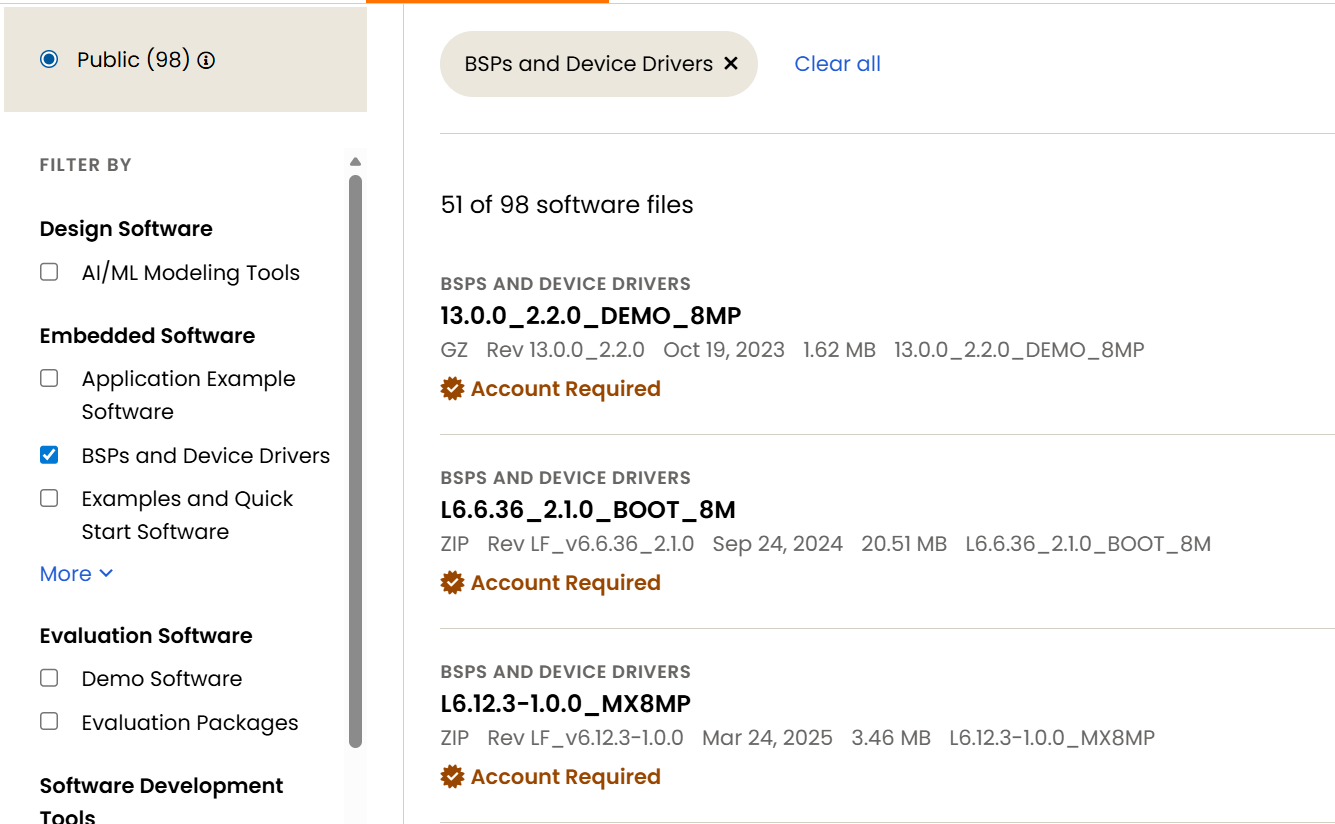
\includegraphics[width=0.8\linewidth]{image.png}
    \caption{Pre-built BSP}
    \label{fig:placeholder}
\end{figure}

\begin{important}
\textbf{However,} the pre-built BSP from NXP is NOT the same as our custom Yocto build. The pre-built images:
\begin{itemize}
    \item Do NOT include our patches/DTS/configurations
    \item But still useful for initial board bring-up/recovery/bench-marking
\end{itemize}
\end{important}

\subsection{Useful NXP Resources}

\begin{itemize}
    \item \textbf{i.MX8M Plus Reference Manual} - Comprehensive hardware documentation 
    \item \textbf{i.MX Linux User's Guide} - teaches you how to build bsp, how to use u-boot
    \item \textbf{i.MX Linux Developer's Guide} - Kernel and driver development
\end{itemize}
\section{JTAG Debugger Setup (For M7 Core Development)}

\subsection{Hardware Connection}

If you plan to work on M7 core development or need to debug the Cortex-M7 real-time processor, you'll need a JTAG debugger connected:


\begin{figure}[H]  
    \centering
    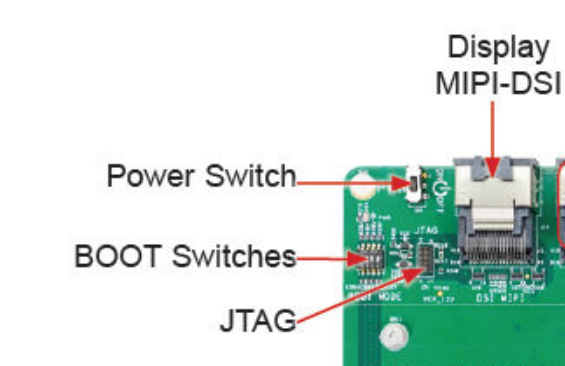
\includegraphics[width=0.5\linewidth]{jtag.png}
    \caption{JTAG Connection to J24 Connector}
    \label{fig:jtag_connection}
\end{figure}

\begin{hardware}
\textbf{JTAG Hardware:}
\begin{itemize}
    \item \textbf{Board Connector:} J24 (20-pin JTAG header)
    \item \textbf{Purpose:} Real-time debugging of Cortex-M7 core (NuttX RTOS/freertos)
\end{itemize}
\end{hardware}


\section{Network Configuration}

\subsection{Ethernet Connection}

The easiest way to transfer files (dtb, elf files etc) is via Ethernet:

\begin{enumerate}
    \item Connect Ethernet cable from board (ETH port) to your network
    \item On the A53 console, check IP address:
    \begin{lstlisting}[language=bash]
root@imx8mpevk:~# ifconfig eth0
eth0: flags=4163<UP,BROADCAST,RUNNING,MULTICAST>  mtu 1500
        inet 192.168.1.XXX  netmask 255.255.255.0  broadcast 192.168.1.255
    \end{lstlisting}
    or
    \begin{lstlisting}[language=bash]
root@imx8mpevk:~# ip a
lo: ....
eth0: ...
eth1:......
    \end{lstlisting}
    
    \item From your development machine/DSO laptop, you can now:
    \begin{itemize}
        \item Use SCP for file transfers: \texttt{scp file.txt root@192.168.1.XXX:/home/root/}
        \item Access via MobaXterm's built-in SFTP browser
    \end{itemize}
\end{enumerate}

\begin{hardware}
\textbf{Ethernet Hardware:}
\begin{itemize}
    \item \textbf{Ethernet Cable:} Connect to eth0 
    \item \textbf{Router:} Self-explanatory \newline
    please ask allan for help otherwise if you need a router etc :)
\end{itemize}
\end{hardware}

\pagebreak

\section{Verifying the Setup}

Once you're logged in, verify the system is working correctly:

\subsection{Check A53 Cores}

\begin{lstlisting}[language=bash]
# Check CPU info
root@imx8mpevk:~# cat /proc/cpuinfo 

# Check if all 4 cores are online
root@imx8mpevk:~# lscpu | grep "On-line"
On-line CPU(s) list:   0-3
\end{lstlisting}

\subsection{Check Yocto Build Version}

\begin{lstlisting}[language=bash]
# Check OS version (should show your custom build)
root@imx8mp-lpddr4-evk:~# cat /etc/os-release
ID=fsl-imx-xwayland
NAME="NXP i.MX Release Distro"
VERSION="6.6-scarthgap (scarthgap)"
VERSION_ID=6.6-scarthgap
VERSION_CODENAME="scarthgap"
PRETTY_NAME="NXP i.MX Release Distro 6.6-scarthgap (scarthgap)"
CPE_NAME="cpe:/o:openembedded:fsl-imx-xwayland:6.6-scarthgap"
root@imx8mp-lpddr4-evk:~#

\end{lstlisting}
\section{Prerequisites for DSO Laptops}


\subsection{Required DSO IT Documentation}
I think the following guides are pretty useful and I missed them out in the first few months of intern and it could have saved a lot of valuable time :

\begin{enumerate}
    \item \textbf{HTTPS Decryption and Certificate Setup}
    \begin{itemize}
        \item Guide: "HTTPS Decryption Onboarding Guide"
        \item \textbf{Why you need this:} you need proper certificates, else Python, Anaconda, Git, Docker, and Yocto builds will fail with SSL/certificate errors.
        \item Follow the guide to install DSO root certificates for all development tools. You should only need 2 certificates the DSO50CA50 and DSOvisbilityCA 
    \end{itemize}
    
    \item \textbf{Software Installation via EPM (Enterprise Package Manager)}
    \begin{itemize}
        \item Guide: "EPM Software Installation Guide"
        \item \textbf{Why you need this:} Many development tools require administrator rights to install. EPM allows you to request and install approved software without admin access.
        \item You'll need to request installation rights for most softwares.
    \end{itemize}
    
    \item \textbf{WSL2 (Windows Subsystem for Linux) Setup}
    \begin{itemize}
        \item Guide: "WSL2 Installation and Configuration"
        \item \textbf{Why you need this:} Yocto builds require a Linux environment. WSL2 is the recommended solution for DSO Windows laptops.
        \item The guide covers: WSL2 installation via EPM, Ubuntu setup, network configuration, and certificate integration.
    \end{itemize}
\end{enumerate}

\begin{docref}
\textbf{Where to Find These Guides:}

DSO Internal Portal > All Knowledge Bases > IT Service > Search for:
\begin{itemize}
    \item "HTTPS Decryption"
    \item "EPM Software Installation"
    \item "WSL2 Setup"
\end{itemize}

If you cannot find these documents or encounter access issues, contact DSO IT Service Desk.
\end{docref}




\chapter{System Architecture}

This chapter explains the overall system architecture, boot flow, and how different components interact. Understanding this is crucial before diving into specific subsystems.

\section{Essential Components for a Bootable Linux System}

Before understanding the boot sequence, you need to know what pieces are required. To have a fully functional Linux system on the i.MX8M Plus, you need \textbf{four essential components}:

\subsection{The Four Required Components}

\begin{enumerate}
    \item \textbf{Bootloader Image (imx-boot)}
    \begin{itemize}
        \item Combined binary containing U-Boot SPL, U-Boot proper, and ARM Trusted Firmware (ATF)
        \item First thing that runs after BootROM
        \item Initializes hardware and loads the kernel
        \item \textbf{Without this:} Board won't boot at all - BootROM won't find anything to execute
    \end{itemize}
    
    \item \textbf{Linux Kernel Image}
    \begin{itemize}
        \item The actual operating system kernel
        \item Manages hardware, memory, processes, and drivers
    \end{itemize}
    
    \item \textbf{Device Tree Blob (.dtb)}
    \begin{itemize}
        \item Hardware description file telling Linux what hardware exists
        \item Describes peripherals, memory map, clocks, GPIOs, I2C devices, etc.
        \item File: \texttt{imx8mp-evk.dtb mainfile imx8mp-evk-dsp.dtb etc}
        \item \textbf{Without this:} Kernel boots but can't initialize hardware - peripherals might not work immediately
    \end{itemize}
    
    \item \textbf{Root Filesystem (rootfs)}
    \begin{itemize}
        \item All files and directories: /bin, /lib, /etc, /usr, applications, libraries
        \item Everything that makes the system usable - shell, utilities, your applications
        \item \textbf{Without this:} Kernel boots but panics with "VFS: Unable to mount root fs"
    \end{itemize}
\end{enumerate}

\begin{important}
\textbf{ALL FOUR components must be present for a successful boot.} Missing any one will cause boot failure at different stages.
\end{important}

\subsection{Where Each Component Lives on eMMC}

\begin{center}
\begin{tabular}{|l|l|l|}
\hline
\textbf{Component} & \textbf{eMMC Location} & \textbf{Filesystem Type} \\
\hline
Bootloader (imx-boot) & Offset 33KB & Raw binary \\
Kernel (Image) & Boot partition (\texttt{mmc 2:1}) & FAT32 \\
Device Tree (.dtb) & Boot partition (\texttt{mmc 2:1}) & FAT32 \\
Root Filesystem & Root partition (\texttt{mmc 2:2}) & ext4 \\
\hline
\end{tabular}
\end{center}

\section{Complete Boot Sequence}

Now that you know what components are needed, I think it will be nice to know how they work together during boot. Understanding this sequence is critical for debugging issues and modifying the system.

\subsection{Boot Flow: Power-On to Login Prompt}

\begin{enumerate}
    \item \textbf{Power On} - Board receives power
    
    \item \textbf{BootROM} (on-chip, immutable)
    \begin{itemize}
        \item Executes from internal ROM (cannot be modified)
        \item Reads boot mode from DIP switches (SW1101)
        \item Looks for bootloader at offset 33KB on eMMC
        \item Loads U-Boot SPL into internal OCRAM
        \item Validates and jumps to U-Boot SPL
    \end{itemize}
    
    \item \textbf{U-Boot SPL} (Secondary Program Loader)
    \begin{itemize}
        \item Minimal bootloader, runs from OCRAM
        \item Initializes DDR RAM (DRAM)
        \item Loads full U-Boot and ATF from eMMC into DDR
        \item Jumps to ARM Trusted Firmware (ATF)
    \end{itemize}
    
    \item \textbf{ARM Trusted Firmware (ATF)}
    \begin{itemize}
        \item Configures secure/non-secure world split
        \item Sets up power domains and PLLs
        \item \textbf{Configurable} - disabled PPLs etc
        \item Loads M7 firmware to TCM memory (if enabled)
        \item Starts M7 core execution (NuttX RTOS)
        \item Jumps to U-Boot proper
    \end{itemize}
    
    \item \textbf{U-Boot Proper} - Full-featured bootloader
    \begin{itemize}
        \item Provides interactive console (press any key to stop autoboot)
        \item Reads boot partition from \texttt{mmc 2:1}
        \item Loads Linux kernel (\texttt{Image}) into DDR
        \item Loads device tree blob (\texttt{imx8mp-evk.dtb}) into DDR
        \item Sets kernel command line parameters (e.g., root partition location)
        \item Jumps to Linux kernel entry point
    \end{itemize}
    
    \item \textbf{Linux Kernel} - Operating system
    \begin{itemize}
        \item Initializes hardware using device tree information
        \item Loads drivers for peripherals (UART, I2C, GPIO, etc.)
        \item Sets up memory management and interrupt handling
        \item Starts init system (systemd)
    \end{itemize}
    
    \item \textbf{Userspace} - Applications and services
    \begin{itemize}
        \item systemd starts all configured services (SSH, networking, monitoring)
        \item Login prompt appears on serial console
        \item System ready for use
    \end{itemize}
\end{enumerate}
\pagebreak
\subsection{Visual Boot Flow}

\begin{verbatim}
    

Power On
    ↓
BootROM (reads DIP switches)
    ↓
U-Boot SPL (initializes DDR)
    ↓
ARM Trusted Firmware (ATF)
    ├─→ Configures power/PLLs
    ├─→ Loads M7 firmware → M7 starts running NuttX
    └─→ Jumps to U-Boot
         ↓
U-Boot Proper
    ├─→ Loads Kernel (Image) from mmc 2:1
    ├─→ Loads Device Tree (.dtb) from mmc 2:1
    └─→ Jumps to Kernel
         ↓
Linux Kernel
    ├─→ Parses device tree
    ├─→ Initializes drivers
    └─→ Mounts rootfs from mmc 2:2
         ↓
Userspace (systemd)
    └─→ Login prompt
    
\end{verbatim}

% TODO: Add a proper flowchart diagram here if needed

\section{Yocto Build Outputs Explained}

When you build a Yocto image, several files are generated. Here's what each one is and when to use it:

\subsection{.wic File - Complete Disk Image}

\begin{itemize}
    \item \textbf{What it is:} A complete disk image containing ALL four components
    \item \textbf{File example:} \texttt{imx-image-full-imx8mpevk.wic}
    \item \textbf{When to use:} Initial board setup or complete system recovery
    \item \textbf{How to flash:}
    \begin{lstlisting}[language=bash]
# Then from your PC:
$ uuu -b emmc .wic file 
    \end{lstlisting}
\end{itemize}

\begin{important}
\textbf{Warning:} Flashing a .wic file will OVERWRITES THE ENTIRE eMMC, including all your configurations and data. Only use this for initial setup or complete recovery.
\end{important}

\subsection{Rootfs Archive - Filesystem Only}

\begin{itemize}
    \item \textbf{What it is:} Just the root filesystem, without bootloader/kernel/DTB
    \item \textbf{Format:} tar.gz compressed archive or ext4 image
    \item \textbf{File example:} \texttt{imx-image-full-imx8mpevk.rootfs.tar.gz}
    \item \textbf{When to use:} Update userspace applications without touching bootloader/kernel
    \item \textbf{Contains:} /bin, /lib, /etc, /usr, your custom applications
\end{itemize}

\subsection{Individual Component Files}

You can also extract/use individual components:

\begin{itemize}
    \item \texttt{imx-boot-imx8mpevk-sd.bin-flash\_evk} - Just the bootloader
    \item \texttt{Image} - Just the kernel
    \item \texttt{imx8mp-evk.dtb} - Just the device tree
\end{itemize}

\begin{docref}
\textbf{For detailed Yocto build instructions:} See Chapter 4: Yocto Build Environment to learn how to build and customize these images.\newline
\textbf{For learning how to flash into emmc/sdcard:} Recommend checking out Universal Update Utility PDF
\end{docref}

\subsection{Update Device Tree Only}

The device tree describes your hardware configuration. Here's the proper workflow for updating it:

\subsubsection{Step 1: Modify and Compile Device Tree on Host PC}

\begin{lstlisting}[language=bash]
# On your development PC:
# Edit your device tree source file (e.g., imx8mp-evk-chyn.dts)
$ vim imx8mp-evk-chyn.dts

# Compile .dts to .dtb using device tree compiler
$ dtc -I dts -O dtb -o imx8mp-evk-chyn.dtb imx8mp-evk-chyn.dts

# Or if you're modifying an existing .dtb, decompile first:
$ dtc -I dtb -O dts -o imx8mp-evk.dts imx8mp-evk.dtb
# All of these can be done on the board as well!
\end{lstlisting}

\subsubsection{Step 2: Transfer to Board}

\begin{lstlisting}[language=bash]
# SCP the compiled .dtb file to the board
$ scp imx8mp-evk-chyn.dtb root@192.168.1.XXX:/tmp/

#I have a separate folder for dts files at /opt/Dts-files
\end{lstlisting}

\subsubsection{Step 3: Place in Boot Partition}

\begin{lstlisting}[language=bash]
# On the board (via SSH or serial console):
root@imx8mp-lpddr4-evk:~# cp /tmp/imx8mp-evk-chyn.dtb /run/media/boot-mmcblk2p1/

\end{lstlisting}

\begin{important}
\textbf{Boot Partition Location:} The boot partition is automatically mounted at \texttt{/run/media/boot-mmcblk2p1/}. This is where all \texttt{.dtb} files must be placed for U-Boot to find them.
\end{important}



\begin{lstlisting}[language=bash]
# Reboot and interrupt U-Boot (press any key during countdown)
root@imx8mp-lpddr4-evk:~# reboot

# In U-Boot console:
=> printenv fdtfile
fdtfile=imx8mp-evk.dtb

# Verify your new .dtb is present on eMMC boot partition:
=> ls mmc 2:1
# Note: Use 'mmc 1:1' if booting from SD card, 'mmc 2:1' for eMMC
      4567 Image
       123 boot.scr
     45678 imx8mp-evk.dtb
     45680 imx8mp-evk-chyn.dtb  <--- Your new device tree

# Set U-Boot to use your custom device tree:
=> setenv fdtfile imx8mp-evk-chyn.dtb

# Save the environment permanently:
=> saveenv
Saving Environment to MMC... Writing to MMC(2)... OK

# Boot with new device tree:
=> boot
\end{lstlisting}

\subsubsection{Step 4: Configure U-Boot to Use New Device Tree}
\begin{figure}
    \centering
    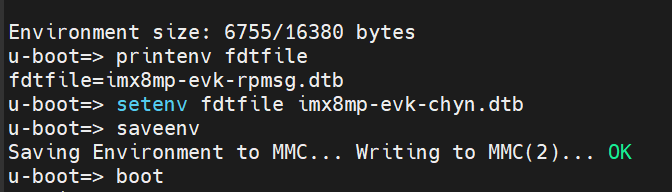
\includegraphics[width=0.75\linewidth]{Uboot saveenv.png}
\end{figure}

\begin{important}
\textbf{Key U-Boot Variable:} The \texttt{fdtfile} environment variable tells U-Boot which device tree blob to load. After using \texttt{setenv}, you MUST run \texttt{saveenv} to make the change persistent across reboots.
\end{important}

\begin{docref}
\textbf{Device Tree Modification Guide:} For detailed information on device tree syntax and how to modify specific peripherals, see CHAPTER 5: DEVICE TREE CONFIGURATION .
\end{docref}


\subsection{Update Rootfs Only}

\begin{lstlisting}[language=bash]
# This is more complex - usually done by:
# 1. Extract rootfs.tar.gz to root partition, OR
# 2. Rebuild and flash entire .wic image

\end{lstlisting}

\textbf{When you need this:} Updated applications, added new libraries, changed configuration files

\begin{important}
\textbf{TLDR (Please update if you find a better workflow):}
\begin{itemize}
    \item For bootloader/ATF changes: Update bootloader only
    \item For kernel/driver changes: Update kernel + DTB
    \item For application changes: Use SCP to copy files directly
    \item For complete system updates: Flash .wic image
\end{itemize}

This saves time by avoiding full reflashes for every change.
\end{important}



\pagebreak
\section{M7 Firmware Loading (Brief Overview)}

The Cortex-M7 core is a real-time processor that can run independently of the A53 cores.

\subsection{M7 Startup Modes}

The M7 core can be started in different ways:

\begin{enumerate}
    \item \textbf{Remoteproc Framework (Linux controlled)}
    \begin{itemize}
        \item M7 is OFF by default after boot
        \item Linux starts M7 via remoteproc subsystem
        \item Firmware loaded from \texttt{/lib/firmware/}
    \end{itemize}
    
    \item \textbf{JTAG Debugger (Development mode)}
    \begin{itemize}
        \item Load firmware directly via JTAG using VS Code + MCUXpresso
        \item Bypasses remoteproc entirely
        \item Used for active development and debugging
        \item Check section 9.2 for more details
    \end{itemize}
\end{enumerate}

\subsection{Quick M7 Control Commands}

\begin{lstlisting}[language=bash]
# Check M7 status
root@imx8mpevk:~# cat /sys/class/remoteproc/remoteproc0/state
offline  # M7 is not running

# Start M7 core
root@imx8mpevk:~# echo start > /sys/class/remoteproc/remoteproc0/state

# Stop M7 core
root@imx8mpevk:~# echo stop > /sys/class/remoteproc/remoteproc0/state

# Load specific elf file from /lib/firmware
root@imx8mpevk:~# echo nuttx-m7-uart4.elf > /sys/class/remoteproc/remoteproc0/firmware 
\end{lstlisting}

\begin{docref}
\textbf{Detailed M7 Development Guide:} For complete information on M7 firmware development, NuttX RTOS setup, JTAG debugging, VS Code configuration, and peripheral drivers, see \textbf{Chapter X: M7 Core Development}.
\end{docref}
\pagebreak
\section{Software Stack by Core}

Here's what runs on each processing unit:

\subsection{Cortex-A53 Cores (Application Processors)}

\begin{itemize}
    \item \textbf{Operating System:} Yocto Linux (custom build)
    \item \textbf{Kernel Version:} Linux 5.15.x (LTS)
    \item \textbf{Init System:} systemd
    \item \textbf{Key Services:}
    \begin{itemize}
        \item Zabbix agent (monitoring)
        \item SSH daemon
        \item Network services
        \item Future: Computer vision applications, AI inference
    \end{itemize}
\end{itemize}

\subsection{Cortex-M7 Core (Real-Time Processor)}

\begin{itemize}
    \item \textbf{Status:} Started manually via remoteproc or JTAG debugger
    \item \textbf{Peripherals Configured:}
    \begin{itemize}
        \item UART4 (console/debugging)
        \item I2C3, I2C5 (sensor communication) , GPIO , SPI etc
        \item 
    \end{itemize}
    \item \textbf{Not implemented:} PX4 flight controller software integration
\end{itemize}

\subsection{NPU (Neural Processing Unit)}

\begin{itemize}
    \item \textbf{Framework:} TensorFlow Lite
    \item \textbf{Delegate:} VX Delegate (Vivante optimized)
    \item \textbf{Status:} Benchmarked, ready for inference workloads
    \item \textbf{Performance:} 2.3 TOPS for INT8 quantized models
\end{itemize}

\subsection{DSP (Digital Signal Processor)}

\begin{itemize}
    \item \textbf{Type:} Cadence Tensilica HiFi4 DSP
    \item \textbf{Status:} Preliminary exploration only
    \item \textbf{Potential Use Cases:} Sensor fusion, audio processing, signal filtering
    \item \textbf{Note:} Not currently utilized - future work item
\end{itemize}
\section{Memory Architecture}

\subsection{Physical Memory Map}

\begin{center}
\begin{tabular}{|l|l|l|}
\hline
\textbf{Address Range} & \textbf{Size} & \textbf{Description} \\
\hline
0x00000000 - 0x0001FFFF & 128 KB & M7 ITCM (Instruction TCM) \\
0x20000000 - 0x2001FFFF & 128 KB & M7 DTCM (Data TCM) \\
0x40000000 - 0x5FFFFFFF & 512 MB & Peripheral registers \\
0x40000000 & -- & DDR Controller \\
0x30400000 & -- & I2C1 \\
0x30A20000 & -- & UART4 (M7 console) \\
0x80000000 - 0xFFFFFFFF & 2 GB & DDR RAM (shared by A53 and M7) \\
\hline
\end{tabular}
\end{center}

\begin{important}
\textbf{Memory Sharing:}
\begin{itemize}
    \item DDR RAM (starting at 0x80000000) is \textbf{shared} between A53 and M7 cores
    \item TCM (ITCM/DTCM) is \textbf{exclusive} to M7 core
    \item Careful memory allocation required to avoid conflicts
    \item Resource Domain Controller (RDC) manages access permissions
\end{itemize}
\end{important}


\section{Inter-Processor Communication (Planned)}

\begin{important}
\textbf{Status:} RPMsg framework explored but not fully implemented.
\end{important}

The plan for A53 <-> M7 communication:
\begin{itemize}
    \item \textbf{Protocol:} RPMsg (Remote Processor Messaging)
    \item \textbf{Transport:} Shared memory in DDR + Mailbox interrupts
    \item \textbf{Use Cases:}
    \begin{itemize}
        \item A53 sends high-level commands to M7 (e.g., "change flight mode")
        \item M7 sends telemetry to A53 (e.g., "current altitude, battery level")
        \item Offload non-time-critical processing from M7 to A53
    \end{itemize}
\end{itemize}

\pagebreak

\section{Resource Domain Controller (RDC)}

The RDC prevents conflicts when multiple cores access the same peripherals:

\subsection{Current RDC Configuration}

\begin{center}
\begin{tabular}{|l|l|}
\hline
\textbf{Peripheral} & \textbf{Owner} \\
\hline
UART1, UART2, UART3 & A53 (Linux) \\
UART4 & M7 (NuttX console) \\
I2C1 & M7 (sensor access) \\
I2C2 & M7 (sensor access) \\
I2C3, I2C4 & A53 (Linux) \\
SPI1 & M7 (future: IMU) \\
GPIO1 & Shared (careful!) \\
\hline
\end{tabular}
\end{center}

\begin{important}
\textbf{RDC Violation = System Crash}

If a core tries to access a peripheral it doesn't own, the system will trigger a bus fault and likely crash. Always verify RDC configuration when adding new peripheral access.
\end{important}


\chapter{Yocto Build Environment}

This chapter covers everything you need to know about building and customizing the Linux BSP for the i.MX8M Plus using the Yocto Project. We'll start with understanding Yocto's structure, then move to practical build instructions.

\begin{important}
\textbf{Current Build Configuration (SD-card):}
\begin{itemize}
    \item \textbf{Yocto Release:} Walnascar (6.12)
    \item \textbf{BSP Version:} imx-6.12.20-2.0.0
    \item \textbf{Machine:} imx8mp-lpddr4-evk
    \item \textbf{Distro:} fsl-imx-xwayland
    \item \textbf{Custom Layer:} meta-chyn
\end{itemize}

Emmc build is using Scarthgap  (6.6)  and works well.
\end{important}

\section{Understanding Yocto Architecture}

Before diving into building, it's crucial to understand how Yocto is organized. Think of it like this:

\subsection{The Yocto Hierarchy}

\begin{enumerate}
    \item \textbf{Layers} (meta-*)
    \begin{itemize}
        \item Top-level organizational units
        \item Each layer is a directory containing recipes, configurations, and patches
        \item Example: \texttt{meta-imx}, \texttt{meta-freescale}, \texttt{meta-chyn}
        \item Layers stack on top of each other (like transparent overlays)
    \end{itemize}
    
    \item \textbf{Recipes} (.bb files)
    \begin{itemize}
        \item Instructions for building a specific package
        \item Example: \texttt{imx-atf\_2.12.bb} tells Yocto how to build ARM Trusted Firmware
        \item Contains: source location, dependencies, compile steps, install instructions
    \end{itemize}
    
    \item \textbf{Recipe Appends} (.bbappend files)
    \begin{itemize}
        \item Modifies an existing recipe without editing the original
        \item Example: \texttt{imx-atf\_\%.bbappend} adds your custom patches to ATF
        \item The \texttt{\%} is a wildcard matching any version
    \end{itemize}
    
    \item \textbf{Packages}
    \begin{itemize}
        \item The compiled output of a recipe (binary, libraries, config files)
        \item Gets installed into the final root filesystem
        \item Example: \texttt{zabbix-agent} package from \texttt{zabbix} recipe
    \end{itemize}
\end{enumerate}

\subsection{Key NXP Layers in Our Build}

\begin{center}
\begin{tabular}{|l|p{8cm}|}
\hline
\textbf{Layer Name} & \textbf{Purpose} \\
\hline
meta-imx & NXP's main i.MX layer - BSP recipes, kernel, bootloader, graphics \\
\hline
meta-freescale & Freescale/NXP common layer - machine configs, u-boot, drivers \\
\hline
poky & Yocto reference distribution - base recipes (gcc, glibc, systemd) \\
\hline
meta-openembedded & Community layer - extra packages (networking, utilities) \\
\hline
meta-chyn & \textbf{YOUR custom layer} - your patches, custom configs, added packages \\
\hline
\end{tabular}
\end{center}

\begin{important}
\textbf{Why create your own layer?}
\begin{itemize}
    \item Keeps your customizations separate from NXP's code
    \item Makes it easy to upgrade to new BSP versions
    \item Your changes are organized and version-controlled
    \item Can be shared with future interns without conflicting with base layers
\end{itemize}
\end{important}

\section{Option 1: Using Pre-Built Images (Quick Start)}

If you just need to get the board running quickly, use NXP's pre-built images.

\subsection{Download Pre-Built BSP}

\begin{enumerate}
    \item Go to: \url{https://www.nxp.com}
    \item Search for: \texttt{i.MX Linux BSP}
    \item Download the latest release for i.MX8M Plus (e.g., \texttt{LF\_v6.6.52-2.2.0\_images\_IMX8MPEVK.zip})
    \item Extract to a working directory:
    \begin{lstlisting}[language=bash]
~/Downloads/LF_v6.6.52-2.2.0_images_IMX8MPEVK/
    \end{lstlisting}
\end{enumerate}

The extracted folder contains:
\begin{itemize}
    \item \texttt{imx-image-full-*.wic.zst} - Complete disk image (compressed)
    \item \texttt{imx-boot-*} - Bootloader binary
    \item \texttt{uuu.auto} - Flash script for UUU tool (just a one line code to run)
\end{itemize}

\subsection{Install UUU (Universal Update Utility)}

UUU is NXP's tool for flashing i.MX boards via USB.

\begin{lstlisting}[language=bash]
# Download from GitHub releases:
# https://github.com/NXPmicro/mfgtools/releases
# For Windows:
# Download uuu.exe and place in your working folder
\end{lstlisting}

\subsection{Flash to eMMC Using UUU}

\begin{enumerate}
    \item Put the board in \textbf{Serial Download Mode}:
    \begin{itemize}
        \item Set DIP switches (SW1101) to: \texttt{0001}
        \item This tells BootROM to wait for USB download instead of booting from eMMC
    \end{itemize}
    
    \item Connect USB cable from board's USB-C port (serial download port J6) to your PC
    
    \item Run UUU:
    \begin{lstlisting}[language=bash]
cd ~/Downloads/LF_v6.6.52-2.2.0_images_IMX8MPEVK/
uuu uuu.auto
    \end{lstlisting}
    
    \item You should see output like:
\end{enumerate}


\begin{figure}[H]
    \centering
    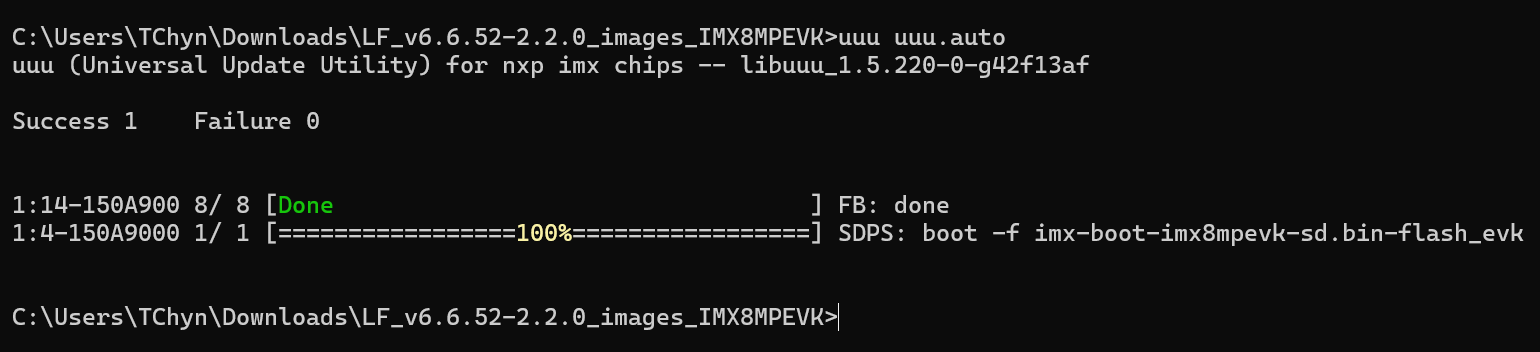
\includegraphics[width=0.75\linewidth]{UUU output.png}
    \caption{UUU output showing progress and success}
    \label{fig:placeholder}
\end{figure}

\section{Option 2: Building from Source (Recommended for Development)}

Building from source gives you full control and allows customization. This is what you'll need for adding custom packages like Zabbix or modifying ATF.

\subsection{Prerequisites (follow the documentation)}

When running WSL2/VM, ensure you have proper setup:

\begin{lstlisting}[language=bash]
# Install required packages
sudo apt-get update
sudo apt-get install build-essential chrpath cpio debianutils diffstat \
  file gawk gcc git iputils-ping libacl1 liblz4-tool locales \
  python3 python3-git python3-jinja2 python3-pexpect python3-pip \
  python3-subunit socat texinfo unzip wget xz-utils zstd efitools
\end{lstlisting}

\begin{docref}
\textbf{Documentation Reference:} i.MX Yocto Project User's Guide - it has all the information you need to get started with building your custom yocto image. Please use this
\end{docref}


\begin{important}
\textbf{Disk Space Warning:} A full \texttt{imx-image-full} build requires \textbf{minimum 550 GB} of free disk space and takes 24-36 hours on my PC with 32 gb of RAM. 
\end{important}

\subsection{Install repo Utility}

\begin{lstlisting}[language=bash]
# Install curl if not already present
sudo apt-get install curl

# Create bin directory and download repo tool
mkdir -p ~/bin
curl https://storage.googleapis.com/git-repo-downloads/repo > ~/bin/repo
chmod a+x ~/bin/repo

# Add to PATH (add to ~/.bashrc to make permanent)
export PATH=~/bin:$PATH
\end{lstlisting}

\pagebreak
\subsection{Download i.MX Yocto BSP Layers}

\begin{lstlisting}[language=bash]
# Create workspace
mkdir ~/imx-yocto-bsp
cd ~/imx-yocto-bsp

# Initialize repo with NXP manifest
repo init -u https://github.com/nxp-imx/imx-manifest \
  -b imx-linux-walnascar \
  -m imx-6.12.20-2.0.0.xml

# When prompted, configure git:
# Name: Your Name
# Email: your.email@example.com

# Download all layers (this takes several minutes)
repo sync
\end{lstlisting}

After \texttt{repo sync} completes, you'll have multiple layer directories:

\begin{lstlisting}
~/imx-yocto-bsp/
├── sources/
│   ├── meta-imx/              # NXP i.MX BSP layer
│   ├── meta-freescale/        # Freescale layer
│   ├── meta-openembedded/     # Community packages
│   ├── poky/                  # Yocto reference distro
│   └── ...more layers...
└── (build directories will be created here)

#at this stage, the following steps might differ in the future. Please take reference from the imx yocto user guide PDF!
\end{lstlisting}

\subsection{Initialize Yocto Build Environment}

\begin{lstlisting}[language=bash]
cd ~/imx-yocto-bsp

# Initialize build environment
DISTRO=fsl-imx-xwayland MACHINE=imx8mp-lpddr4-evk \
  source imx-setup-release.sh -b build-xwayland
\end{lstlisting}

\textbf{What this does:}
\begin{itemize}
    \item Creates \texttt{build-xwayland/} directory with configuration
    \item Sets up environment variables for BitBake
    \item Generates \texttt{conf/local.conf} and \texttt{conf/bblayers.conf}
\end{itemize}

\begin{important}
\textbf{DISTRO Options Explained:}
\begin{itemize}
    \item \texttt{fsl-imx-wayland} - Pure Wayland graphics (no X11 compatibility)
    \item \texttt{fsl-imx-xwayland} - Wayland + XWayland 
    \item \texttt{fsl-imx-fb} - Framebuffer only (no Wayland/X11)
\end{itemize}

\textbf{What is X11 vs Wayland?}
\begin{itemize}
    \item \textbf{X11} - Older Linux display system, supports legacy desktop apps
    \item \textbf{Wayland} - Modern, faster, more secure display protocol
    \item \textbf{XWayland} - Compatibility layer that runs X11 apps on Wayland
\end{itemize}

For i.MX8MP, use \texttt{fsl-imx-xwayland} for best compatibility with both old and new applications. In my experience, its not a lot of new packages downloaded, so leaving it out is also fine
\end{important}

After initialization, you'll see the EULA agreement:
\begin{figure}[H]
    \centering
    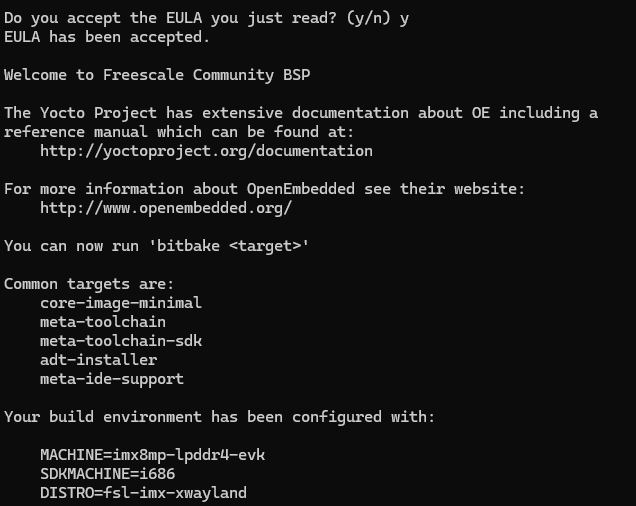
\includegraphics[width=0.75\linewidth]{eula agreement.png}
    \caption{EULA agreement, with build instructions}
    \label{fig:placeholder}
\end{figure}

\subsection{Choose Image Type}

Yocto provides several image recipes depending on your needs:

\begin{center}
\begin{tabular}{|l|p{7cm}|}
\hline
\textbf{Image Recipe} & \textbf{Description} \\
\hline
core-image-minimal & Absolute minimum - boots to shell, nothing else \\
\hline
core-image-base & Console-only with full hardware support \\
\hline
imx-image-core & i.MX test applications for Wayland \\
\hline
imx-image-multimedia & GUI support, multimedia codecs, no Qt \\
\hline
imx-image-full & \textbf{Everything} - Qt6, ML tools, multimedia (what I did) \\
\hline
\end{tabular}
\end{center}

\begin{important}
\textbf{Build Time:}
\begin{itemize}
    \item \texttt{imx-image-core} - 2-4 hours, ~100 GB (unsure)
    \item \texttt{imx-image-full} - 24-36 hours, ~550 GB
\end{itemize}

\end{important}

\subsection{Build the Image}

\begin{lstlisting}[language=bash]
# Make sure you're in the build directory (build-xwayland or whatever you named it)
cd ~/imx-yocto-bsp/build-xwayland

# Start the build (this will take hours)
bitbake imx-image-full
\end{lstlisting}

BitBake will:
\begin{enumerate}
    \item Download all source code (Linux kernel, U-Boot, ATF, packages)
    \item Compile everything from scratch
    \item Generate root filesystem
    \item Package everything into deployable images
\end{enumerate}


\subsection{Optimize Build Performance}
One of the small minor problems i faced was my pc crashing in the middle of builds.
Edit \texttt{build-xwayland/conf/local.conf} to limit parallel jobs if your machine struggles:

\begin{lstlisting}[language=bash]
nano conf/local.conf

# Add these lines (adjust numbers based on your CPU):
BB_NUMBER_THREADS = "5"      # BitBake parallel tasks
PARALLEL_MAKE = "-j5"       # Make parallel compilation
\end{lstlisting}

\textbf{Guidelines:}
\begin{itemize}
    \item \texttt{BB\_NUMBER\_THREADS} - Number of recipes BitBake builds in parallel
    \item \texttt{PARALLEL\_MAKE} - Number of compiler threads per recipe
\end{itemize}

\subsection{Troubleshooting Build Errors}

If a build fails, you can clean and rebuild specific packages:

\begin{lstlisting}[language=bash]
# Clean a specific package (removes all build artifacts)
bitbake -c cleanall <package-name>

# Rebuild just that package to see detailed errors
bitbake <package-name>

\end{lstlisting}

Common error scenarios:
\begin{itemize}
    \item \textbf{Fetch errors} - Network issues, check internet connection
    \item \textbf{Compilation errors} - Missing dependencies, check package logs
    \item \textbf{Disk space errors} - Build partition full, free up space
\end{itemize}


\subsection{Build Output Location}

After successful build, your images are in:

\begin{lstlisting}[language=bash]
~/imx-yocto-bsp/build-xwayland/tmp/deploy/images/imx8mp-lpddr4-evk/

# Key files:
imx-image-full-imx8mp-lpddr4-evk.wic.zst    # Complete disk image (compressed)
imx-image-full-imx8mp-lpddr4-evk.rootfs.tar.gz  # Root filesystem
imx-boot-imx8mp-lpddr4-evk-sd.bin-flash_evk     # Bootloader
\end{lstlisting}
\section{Adding Custom Packages (Zabbix Example)}

One of the key advantages of building from source is adding custom packages. Before adding any package, you need to verify it exists in your Yocto layers and is compatible with your BSP version.

\subsection{Step 1: Search OpenEmbedded Layer Index}

Before modifying your build configuration, always check if the package exists and which layer provides it:

\begin{enumerate}
    \item Go to: \url{https://layers.openembedded.org/layerindex/branch/master/layers/}
    
    \item Select your Yocto branch from the dropdown (e.g., \textbf{walnascar} for our build)
    
    \item Search for your package (e.g., "zabbix")
\end{enumerate}


\begin{figure}
    \centering
    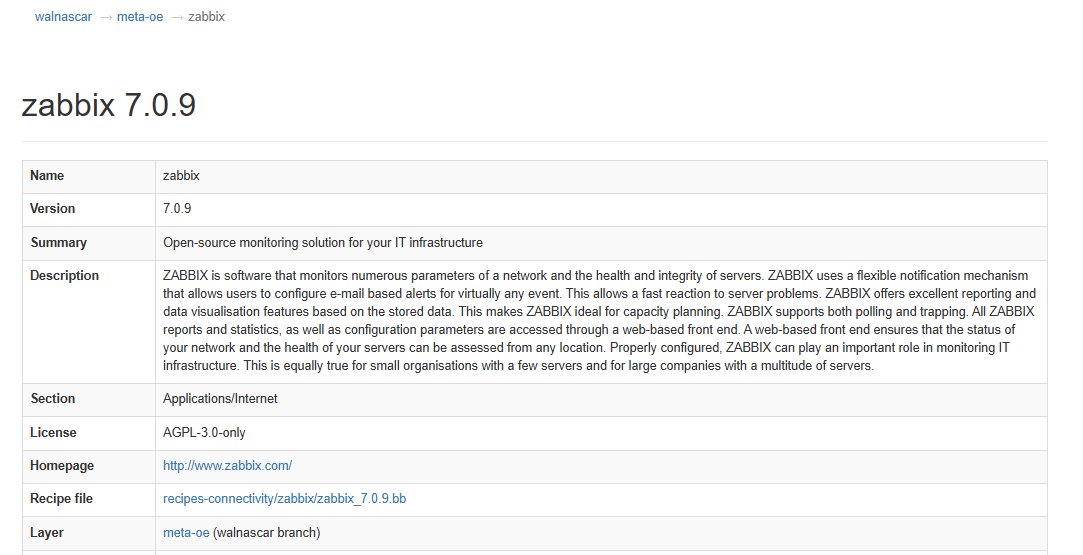
\includegraphics[width=0.75\linewidth]{zabbix layer.png}
    \caption{Zabbix Package in OpenEmbedded Layer Index}
    \label{fig:placeholder}
\end{figure}
From the search results, you can see:

\begin{itemize}
    \item \textbf{Name:} zabbix
    \item \textbf{Version:} 7.0.9
    \item \textbf{Layer:} meta-oe (walnascar branch) 
    \item \textbf{Recipe file:} \texttt{recipes-connectivity/zabbix/zabbix\_7.0.9.bb}
    \item \textbf{Summary:} Open-source monitoring solution for IT infrastructure
\end{itemize}

\begin{important}
\textbf{Key Information to Check:}
\begin{enumerate}
    \item \textbf{Layer name} - Which layer provides this package?
    \item \textbf{Branch compatibility} - Is it available in your Yocto version (walnascar)?
    \item \textbf{Recipe location} - Helps you find it if you need to inspect or modify
\end{enumerate}
\end{important}

\subsection{Step 2: Verify Layer is Already Included}

Check if the required layer is already part of your build:

\begin{lstlisting}[language=bash]
cd ~/imx-yocto-bsp/build-xwayland

# List all layers in your build
bitbake-layers show-layers
\end{lstlisting}

You should see output like:

\begin{lstlisting}
layer                 path                                      priority
==========================================================================
meta                  /home/user/imx-yocto-bsp/sources/poky/meta  5
meta-poky             /home/user/.../poky/meta-poky               5
meta-oe               /home/user/.../meta-openembedded/meta-oe    6  <-- HERE!
meta-python           /home/user/.../meta-openembedded/meta-python 7
meta-networking       /home/user/.../meta-openembedded/meta-networking 5
meta-imx              /home/user/.../meta-imx                     8
...
\end{lstlisting}

\begin{itemize}
    \item  \textbf{Layer exists} - Zabbix is in \texttt{meta-oe}, which is already included in the NXP BSP manifest
    \item ✅ \textbf{Compatible branch} - walnascar branch has zabbix 7.0.9
    \item ✅ \textbf{Ready to use} - Can add directly to \texttt{IMAGE\_INSTALL}
\end{itemize}

\subsection{Step 3: Add Package to Image}

Since \texttt{meta-oe} is already in our build and zabbix exists in the walnascar branch, we can simply add it:

\begin{lstlisting}[language=bash]
nano ~/imx-yocto-bsp/build-xwayland/conf/local.conf

# Add at the end of the file:
IMAGE_INSTALL:append = " zabbix zabbix-agent"
\end{lstlisting}

\subsection{Step 4: Rebuild Image}

\begin{lstlisting}[language=bash]
bitbake imx-image-full
\end{lstlisting}

BitBake will:
\begin{enumerate}
    \item Fetch zabbix source code (version 7.0.9)
    \item Compile zabbix and zabbix-agent
    \item Install into root filesystem
    \item Repackage the image
\end{enumerate}

\subsection{What If the Package Doesn't Exist?}

If you search for a package and it's \textbf{not found} or \textbf{not in any layer you have}, you have three options:

\subsubsection{Option 1: Add the Required Layer}

If the package exists in a layer not included in your build:

\begin{lstlisting}[language=bash]
# Example: Package is in meta-networking (usually already included)
cd ~/imx-yocto-bsp/build-xwayland

# Add the layer
bitbake-layers add-layer ../sources/meta-openembedded/meta-networking

# Verify it was added
bitbake-layers show-layers | grep networking
\end{lstlisting}

\subsubsection{Option 2: Create Your Own Recipe}

If the package doesn't exist in any OpenEmbedded layer, you'll need to create a recipe in your custom layer:

\begin{lstlisting}[language=bash]
# Create recipe in meta-chyn
mkdir -p ~/imx-yocto-bsp/sources/meta-chyn/recipes-custom/mypackage
cd ~/imx-yocto-bsp/sources/meta-chyn/recipes-custom/mypackage

# Create recipe file
vim mypackage_1.0.bb
\end{lstlisting}

Basic recipe template (refer to other template for better visualisation):

\begin{lstlisting}[language=python]
SUMMARY = "My custom package"
DESCRIPTION = "Description of what this does"
LICENSE = "MIT"
LIC_FILES_CHKSUM = "file://LICENSE;md5=..."

SRC_URI = "https://example.com/mypackage-1.0.tar.gz"
SRC_URI[sha256sum] = "abc123..."

inherit autotools
# or: inherit cmake
# or: inherit setuptools3 (for Python)

do_install() {
    install -d ${D}${bindir}
    install -m 0755 myprogram ${D}${bindir}/
}
\end{lstlisting}

\subsubsection{Option 3: Install at Runtime}

For quick testing, you can install packages directly on the running system:

\begin{lstlisting}[language=bash]


# Use opkg if available (but opkg needs to be set up)
opkg update
opkg install <package-name>

# Or compile from source manually on the board using git/wget
\end{lstlisting}

\begin{important}
\textbf{Best Practice:} Always use the Layer Index first. Creating custom recipes should be a last resort - most packages you need already exist in OpenEmbedded layers.
\end{important}

\section{Creating Your Custom Layer}

For more complex customizations (patches, custom configs), create your own layer.

\subsection{Create meta-chyn Layer}

\begin{lstlisting}[language=bash]
cd ~/imx-yocto-bsp/build-xwayland

# Create layer structure
bitbake-layers create-layer ../sources/meta-chyn

# Add layer to build
bitbake-layers add-layer ../sources/meta-chyn

# Verify layer is added
bitbake-layers show-layers
\end{lstlisting}

Your layer structure:

\begin{lstlisting}
sources/meta-chyn/
├── conf/
│   └── layer.conf              # Layer configuration
├── recipes-example/
│   └── example/
│       └── example_0.1.bb      # Example recipe
└── README
\end{lstlisting}

\section{Creating patches for ARM Trusted Firmware}

This section shows how to modify ATF to add custom power management features. This is how the low-power suspend mode optimizations were implemented.

\subsection{Goal}

We want to:
\begin{itemize}
    \item Keep M7 core alive during Linux suspend (using LPA flags)
    \item Add A53→M7 notification helpers via GIR (General Interrupt Register)
    \item Package changes properly using Yocto workflow
\end{itemize}

\subsection{Use devtool to Modify ATF}

\texttt{devtool} is Yocto's development workflow tool - it sets up a workspace for editing source code.

\begin{lstlisting}[language=bash]
cd ~/imx-yocto-bsp/build-xwayland

# Extract ATF source to workspace
devtool modify imx-atf

# Navigate to ATF source
cd workspace/sources/imx-atf
\end{lstlisting}

Now you have the full ATF source code ready for editing in \texttt{workspace/sources/imx-atf/}.

\subsection{Make Your Changes}

Edit the file where power management happens:

\begin{lstlisting}[language=bash]
nano plat/imx/imx8m/gpc_common.c
\end{lstlisting}

\textbf{Add GIR helper functions:}

\begin{lstlisting}[language=c]
#include <platform_def.h>
#ifndef IMX_MU_BASE
#define IMX_MU_BASE U(0x30AA0000) /* A-side MU base on i.MX8MP */
#endif

/* Helper: Notify M7 via GIR0 doorbell */
static void imx_notify_m4_set_db(void)
{
    /* Set GIR0 bit and enable */
    mmio_setbits_32(IMX_MU_BASE + 0x24, BIT(19) | BIT(31));
}

/* Helper: Clear GIP0 after M7 processes notification */
static void imx_notify_m4_clear_db(void)
{
    mmio_setbits_32(IMX_MU_BASE + 0x20, BIT(31));
}
\end{lstlisting}

\textbf{Hook into suspend/resume path:}

Find the \texttt{imx\_set\_sys\_wakeup()} function and add:

\begin{lstlisting}[language=c]
/* Enable MU wakeup */
if (imx_is_m4_enabled()) {
    mmio_clrbits_32(IMX_GPC_BASE + gpc_imr_offset[last_core] + 0x8, BIT(24));

    if (imx_m4_lpa_active()) {
        if (pdn) {
            /* Entering low power - notify M7 */
            imx_notify_m4_set_db();
        } else {
            /* Exiting low power - clear notification */
            imx_notify_m4_clear_db();
        }
    }
}
\end{lstlisting}

\subsection{Commit Your Changes}

\begin{lstlisting}[language=bash]
cd ~/imx-yocto-bsp/build-xwayland/workspace/sources/imx-atf

# Stage and commit your changes
git add plat/imx/imx8m/gpc_common.c
git commit -m "imx8mp: add GIR helpers for A53-M7 suspend coordination"
\end{lstlisting}

\subsection{Handle Build Artifacts (if present)}

Sometimes devtool workspace has build artifacts that shouldn't be committed:

\begin{lstlisting}[language=bash]
# Ignore build directories
echo "build-optee/" >> .gitignore
git add .gitignore
git commit -m "Ignore build-optee artifacts"
\end{lstlisting}

\subsection{Finish devtool and Create Patch}

This command generates a patch and creates a bbappend file in your layer:

\begin{lstlisting}[language=bash]
cd ~/imx-yocto-bsp/build-xwayland

# Finish devtool session - generates patch in meta-chyn
devtool finish imx-atf ../sources/meta-chyn
\end{lstlisting}

This creates:

\begin{lstlisting}
sources/meta-chyn/recipes-bsp/imx-atf/
├── imx-atf_%.bbappend                     # Recipe append
└── imx-atf/
    ├── 0001-imx8mp-add-GIR-helpers-for-suspend.patch
    └── 0002-Ignore-build-optee-artifacts.patch
\end{lstlisting}

\subsection{Add Required Patch Headers}

Yocto QA requires patches to have proper headers. Add \texttt{Upstream-Status} tag:

\begin{lstlisting}[language=bash]
cd ~/imx-yocto-bsp/sources/meta-chyn/recipes-bsp/imx-atf/imx-atf/

# Edit patch file manually or use sed:
sed -i '/^Subject:/a Upstream-Status: Inappropriate [i.MX8MP BSP-specific]\nSigned-off-by: Your Name <you@example.com>' \
  0001-imx8mp-add-GIR-helpers-for-suspend.patch
\end{lstlisting}

The patch should now have headers like:

\begin{lstlisting}
From abc123def456...
Subject: [PATCH] imx8mp: add GIR helpers for A53-M7 suspend coordination
Upstream-Status: Inappropriate [i.MX8MP BSP-specific low-power behavior]
Signed-off-by: Your Name <you@example.com>
---
 plat/imx/imx8m/gpc_common.c | 20 ++++++++++++++++++++
 1 file changed, 20 insertions(+)
\end{lstlisting}

\subsection{Rebuild ATF with Patches}

\begin{lstlisting}[language=bash]
cd ~/imx-yocto-bsp/build-xwayland

# Clean ATF and imx-boot to force rebuild
bitbake -c cleansstate imx-atf imx-boot

# Rebuild with patches applied
bitbake imx-boot
\end{lstlisting}

\subsection{Verify Patches Were Applied}

\begin{lstlisting}[language=bash]
# Check patch log
less tmp/work/*/imx-atf/*/temp/log.do_patch
# Look for "Applying patch 0001-..." messages

# Verify your code is in the source
grep -n "imx_notify_m4_set_db" \
  tmp/work/*/imx-atf/*/git/plat/imx/imx8m/gpc_common.c
\end{lstlisting}

\subsection{Extract and Flash Updated Bootloader}

\begin{lstlisting}[language=bash]
# New imx-boot is in:
cd ~/imx-yocto-bsp/build-xwayland/tmp/deploy/images/imx8mp-lpddr4-evk/

# Flash to SD card (example):
sudo dd if=imx-boot-imx8mp-lpddr4-evk-sd.bin-flash_evk \
        of=/dev/sdX bs=1K seek=33 conv=fsync

# Or for eMMC via UUU - see Chapter 2 for details
\end{lstlisting}

\section{Repository Directory Structure (for Reference)}

Understanding where code lives in Linux kernel and ATF repositories:

\subsection{Linux Kernel Structure}
\begin{verbatim}
linux/
├── arch/                      # Architecture-specific code
│   ├── arm64/                 # A53 cores live here
│   │   ├── boot/dts/          # Device trees
│   │   │   └── freescale/     # i.MX8MP device trees here!
│   │   ├── kernel/            # Low-level ARM64 code
│   │   └── mm/                # Memory management
│   └── arm/                   # 32-bit ARM (not used on A53)
│
├── drivers/                   # Hardware drivers
│   ├── i2c/                   # I2C subsystem
│   ├── spi/                   # SPI subsystem
│   ├── gpu/                   # Graphics drivers
│   └── soc/imx/               # i.MX-specific drivers
│
└── include/
    └── dt-bindings/           # Device tree constants

\end{verbatim}
\subsection{ARM Trusted Firmware Structure}

\begin{verbatim}
    

arm-trusted-firmware/
├── plat/                               # Platform-specific code
│   └── imx/                            # NXP i.MX platforms
│       ├── imx8m/                      # i.MX8M family
│       │   ├── imx8mp/                 # i.MX8M Plus specific
│       │   │   ├── gpc.c               # Power controller (I modified this!)
│       │   │   └── imx8mp_bl31_setup.c # Boot setup
│       │   └── gpc_common.c            # Common GPC code
│       └── common/                     # Common i.MX code
│
└── include/
    └── plat/imx/                       # i.MX headers
\end{verbatim}

\begin{docref}
\textbf{For detailed suspend implementation:} See AN13400 i.MX 8M Low Power Design By M Core Running In System
\end{docref}

\chapter{Device Tree Configuration}

Device tree is the foundation of hardware configuration in embedded Linux. This chapter covers everything from basic syntax to practical examples of adding sensors to the i.MX8M Plus.

\section{What is Device Tree?}

\subsection{Purpose and Overview}

Device tree is a data structure that describes hardware to the Linux kernel. Instead of hardcoding hardware information in the kernel, device tree provides a flexible, human-readable way to tell Linux:

\begin{itemize}
    \item What hardware exists on the board
    \item Where peripherals are located (memory addresses, I2C addresses, etc.)
    \item How to configure them (clock frequencies, pin assignments, power supplies)
    \item How devices are connected (which GPIO pins, which I2C bus, etc.)
\end{itemize}

\begin{important}
\textbf{Key Concept:} Device tree does NOT contain drivers. It only describes hardware. The Linux kernel matches device tree nodes to appropriate drivers using the \texttt{compatible} property.
\end{important}

\subsection{File Types}

\begin{center}
\begin{tabular}{|l|l|p{6cm}|}
\hline
\textbf{Extension} & \textbf{Type} & \textbf{Description} \\
\hline
.dts & Device Tree Source & Human-readable text file you edit \\
\hline
.dtsi & Device Tree Source Include & Reusable chunks included in .dts files \\
\hline
.dtb & Device Tree Blob & Compiled binary that U-Boot loads \\
\hline
.dtbo & Device Tree Blob Overlay & Binary overlay applied at runtime. It only replaces certain portion of a targeted device tree \\
\hline
\end{tabular}
\end{center}

\textbf{Typical structure for i.MX8M Plus:}

\begin{verbatim}
imx8mp.dtsi               <- SoC-level definitions (CPU, memory map)
  |
  +-- imx8mp-evk.dtsi     <- EVK board common features
       |
       +-- imx8mp-evk.dts      <- Base board configuration
       +-- imx8mp-evk-rpmsg.dts <- Board with RPMsg enabled
       +-- imx8mp-evk-chyn.dts  <- YOUR custom configuration
\end{verbatim}
\begin{docref}
\textbf{Additional Resources:}
\begin{itemize}
    \item \textbf{Device Tree Syntax:} NXP Application Note AN5125 "Introduction to Device Trees" - comprehensive syntactical reference
    \item \textbf{Device Tree Overlays:} \url{https://community.nxp.com/t5/i-MX-Processors-Knowledge-Base/How-to-use-linux-device-tree-overlay-from-u-boot-and-apply-it/ta-p/1896858}
\end{itemize}
\end{docref}

\section{Checking Your Current Configuration}

\subsection{Which DTB is Currently Loaded?}

\textbf{From U-Boot}

\begin{lstlisting}[language=bash]
# Stop autoboot and check environment variable
u-boot=> printenv fdtfile
fdtfile=imx8mp-evk-rpmsg.dtb

# Check where device tree is loaded in memory
u-boot=> printenv fdt_addr
fdt_addr=0x43000000
\end{lstlisting}

\subsection{Available DTB Files}

\textbf{From U-Boot - List eMMC boot partition:}

\begin{lstlisting}[language=bash]
u-boot=> ls mmc 2:1
 35631616   Image
    84282   imx8mp-evk.dtb
    65300   imx8mp-evk-rpmsg.dtb
    84266   imx8mp-evk-flexcan2.dtb
    # ... more files
\end{lstlisting}

\begin{important}
\textbf{Boot Partition Location:}
\begin{itemize}
    \item \textbf{From U-Boot:} \texttt{mmc 2:1} (eMMC) or \texttt{mmc 1:1} (SD card)
    \item \textbf{From Linux:} \texttt{/run/media/boot-mmcblk2p1/} (auto-mounted boot partition)
\end{itemize}

To check which is which:
\begin{lstlisting}[language=bash]
u-boot=> mmc list
FSL_SDHC: 1
FSL_SDHC: 2 (eMMC)
\end{lstlisting}
\end{important}

\begin{gitref}
\textbf{All DTS files can be found in:}

\url{https://github.com/yulyuri/firmware-and-dts/blob/master/SCP%20files}
\end{gitref}
\section{Device Tree Compiler (dtc)}

The device tree compiler (\texttt{dtc}) converts between human-readable (\texttt{.dts}) and binary (\texttt{.dtb}) formats.

\subsection{Essential dtc Flags}

\begin{center}
\begin{tabular}{|l|p{9cm}|}
\hline
\textbf{Flag} & \textbf{Purpose} \\
\hline
-I  & Input format: dts, dtb, fs (filesystem), yaml \\
\hline
-O  & Output format: dts, dtb, yaml \\
\hline
-o  & Output file path \\
\hline
-@ & Keep/generate symbols (needed for overlays and readable labels) \\
\hline
-s & Sort nodes alphabetically (useful for comparing trees) \\
\hline
\end{tabular}
\end{center}

\subsection{Common dtc Operations}

\textbf{Decompile DTB to readable DTS:}

\begin{lstlisting}[language=bash]
# Decompile a single DTB file
dtc -I dtb -O dts -o /tmp/imx8mp-evk.dts \
    /run/media/boot-mmcblk2p1/imx8mp-evk.dtb

# Decompile ALL DTB files at once (very useful!)
for f in /run/media/boot-mmcblk2p1/*.dtb; do 
    dtc -s -I dtb -O dts -o "/tmp/$(basename "${f%.dtb}").dts" "$f"
done
\end{lstlisting}

\textbf{Compile DTS back to DTB:}

\begin{lstlisting}[language=bash]
# Basic compilation
dtc -I dts -O dtb -o /tmp/imx8mp-evk-test.dtb /tmp/imx8mp-evk.dts

# With symbol preservation (recommended)
dtc -@ -I dts -O dtb -o /tmp/imx8mp-evk-chyn.dtb /tmp/imx8mp-evk-chyn.dts
\end{lstlisting}

\subsection{Comparing Device Trees}

You can use \texttt{dtc} with the \texttt{-s} (sort) flag to compare two device tree configurations:

\begin{lstlisting}[language=bash]
# Decompile both with sorting
dtc -s -I dtb -O dts -o /tmp/rpmsg.dts \
    /run/media/boot-mmcblk2p1/imx8mp-evk-rpmsg.dts

dtc -s -I dtb -O dts -o /tmp/rpmsg-lpv.dts \
    /run/media/boot-mmcblk2p1/imx8mp-evk-rpmsg-lpv.dts

# Compare to see differences
diff /tmp/rpmsg.dts /tmp/rpmsg-lpv.dts | less
\end{lstlisting}

\textbf{Example finding:} Comparing \texttt{rpmsg.dtb} vs \texttt{rpmsg-lpv.dtb} shows that LPV (Low Power Voice) removes:
\begin{itemize}
    \item \texttt{fsl,enable-lpa} property
    \item \texttt{fsl,rpmsg-in} node
\end{itemize}

This tells you how LPV is implemented at the hardware level!

% TODO: Add screenshot showing diff output
% \begin{figure}[H]
% \centering
% \includegraphics[width=0.9\textwidth]{dtb_diff_example.png}
% \caption{Comparing device trees to understand feature differences}
% \label{fig:dtb_diff}
% \end{figure}

\section{Device Tree Syntax Fundamentals}

\subsection{Nodes and Hierarchy}

Device tree is organized as a tree of nodes:

\begin{lstlisting}[language=c]
/ {                              // Root node
    compatible = "fsl,imx8mp-evk", "fsl,imx8mp";
    
    soc@0 {                      // SoC container node
        i2c@30ad0000 {          // I2C5 controller node
            compatible = "fsl,imx8mp-i2c";
            reg = <0x30ad0000 0x10000>;
            
            sensor@68 {          // Device on I2C bus
                compatible = "invensense,mpu6050";
                reg = <0x68>;    // I2C address
            };
        };
    };
};
\end{lstlisting}

\textbf{Node naming convention:} \texttt{name@unit-address}
\begin{itemize}
    \item \texttt{name} - Descriptive name (i2c, sensor, gpio, etc.)
    \item \texttt{@unit-address} - Device address (MMIO base, I2C address, etc.)
\end{itemize}

\subsection{Properties}

Properties are key-value pairs that describe node characteristics:

\begin{lstlisting}[language=c]
sensor@68 {
    // String property
    compatible = "invensense,mpu6050";
    
    // Integer property (32-bit cells)
    reg = <0x68>;
    
    // Multiple strings
    pinctrl-names = "default", "sleep";
    
    // Boolean flag (presence = true)
    regulator-always-on;
    
    // Reference to another node (phandle)
    vdd-supply = <&buck2>;
    interrupt-parent = <&gpio1>;
    
    // Array of integers
    clocks = <&clk IMX8MP_CLK_I2C5_ROOT>;
};
\end{lstlisting}

\subsection{Labels and Phandles}

Labels let you reference nodes from anywhere in the device tree:

\begin{lstlisting}[language=c]
// Define a label
i2c5: i2c@30ad0000 {
    compatible = "fsl,imx8mp-i2c";
    // ... properties
};

// Reference it later
&i2c5 {
    clock-frequency = <100000>;  // Override/add properties
    
    my_sensor@68 {
        // Add child node
    };
};

// Or use as phandle in properties
sensor {
    i2c-bus = <&i2c5>;
};
\end{lstlisting}


\subsection{Interrupts}

Interrupt specification format is defined by the interrupt controller:

\begin{lstlisting}[language=c]
// ARM GIC (most common on i.MX8MP)
sensor@68 {
    interrupt-parent = <&gic>;
    interrupts = <GIC_SPI 76 IRQ_TYPE_LEVEL_HIGH>;
    // Which expands to: <0 76 4>
    //   0 = SPI (Shared Peripheral Interrupt)
    //   76 = interrupt number
    //   4 = level-high trigger
};

// GPIO interrupts
sensor@68 {
    interrupt-parent = <&gpio1>;
    interrupts = <12 IRQ_TYPE_EDGE_FALLING>;
};
\end{lstlisting}

\subsection{Pin Control (i.MX Specific)}

Pin muxing is handled by \texttt{pinctrl} groups:

\begin{lstlisting}[language=c]
// Define pin group in IOMUXC node
&iomuxc {
    pinctrl_i2c5: i2c5grp {
        fsl,pins = <
            // MUX_REG PAD_REG SELECT_INPUT ALT DAISY PAD_CTL
            MX8MP_IOMUXC_SPDIF_TX__I2C5_SCL  0x400001c3
            MX8MP_IOMUXC_SPDIF_RX__I2C5_SDA  0x400001c3
        >;
    };
};

// Use pin group in device node
&i2c5 {
    pinctrl-names = "default";
    pinctrl-0 = <&pinctrl_i2c5>;
};
\end{lstlisting}

The macros expand to 6 values:
\begin{itemize}
    \item MUX register offset
    \item PAD control register offset  
    \item SELECT\_INPUT (daisy chain) register offset
    \item ALT function number (which peripheral uses this pin)
    \item Daisy chain value
    \item PAD control value (drive strength, pull-up/down, etc.)
\end{itemize}

These are defined in \texttt{arch/arm64/boot/dts/freescale/imx8mp-pinfunc.h}.

\section{Complete Workflow: Adding an IMU Sensor}

Let's walk through a real example: adding the MPU-6050/6500 IMU to I2C5 on connector J22.

\begin{gitref}
\textbf{Complete Working Example:}

\textbf{File:} \texttt{imx8mp-evk-chyn-m7.dts} \\
\textbf{Lines:} 1787-1808 (MPU-6050 sensor configuration)

\url{https://github.com/yulyuri/firmware-and-dts/blob/master/SCP%20files/imx8mp-evk-chyn-m7.dts}

This file contains the complete I2C5 controller setup with MPU-6050 sensor node, including pin muxing and power supply configuration.
\end{gitref}

\subsection{Step 1: Identify Hardware Connections}
\begin{figure}[H]
    \centering
    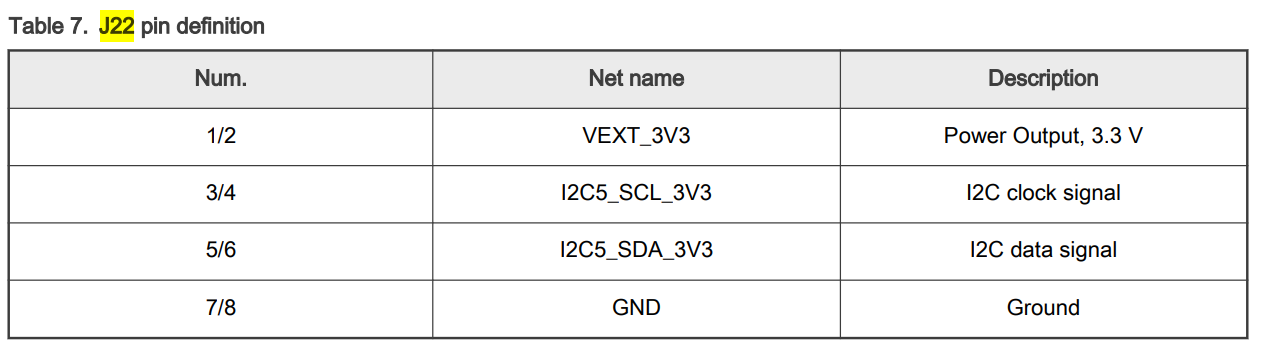
\includegraphics[width=0.75\linewidth]{i2c header pinouts.png}
    \caption{i2c header pinouts}
    \label{fig:placeholder}
\end{figure}
Check the i.MX8MP EVK Hardware User Guide for J22 pinout:

\begin{itemize}
    \item J22 is connected to I2C5 lines (SPDIF\_TX and SPDIF\_RX pins muxed to I2C)
    \item SoC I2C5 base address: 0x30AD0000
    \item Linux typically enumerates this as \texttt{i2c-4} (check with \texttt{ls /sys/bus/i2c/devices/})
\end{itemize}

\textbf{Verify I2C mapping:}

\begin{lstlisting}[language=bash]
root@imx8mp-lpddr4-evk:~# cat /sys/bus/i2c/devices/i2c-4/name

# Cross-reference with i.MX8MP Reference Manual:
# 0x30AD0000 = I2C5
\end{lstlisting}

\subsection{Step 2: Find and Extract Base Device Tree}

\begin{lstlisting}[language=bash]
# Decompile the base DTB you want to modify
dtc -I dtb -O dts -o /tmp/imx8mp-evk-rpmsg.dts \
    /run/media/boot-mmcblk2p1/imx8mp-evk-rpmsg.dtb

# Copy to working directory for editing or scp to host pc/laptop for editing
cp /tmp/imx8mp-evk-rpmsg.dts /tmp/imx8mp-evk-chyn.dts
\end{lstlisting}

\subsection{Step 3: Locate I2C5 Controller Node}

Search for the I2C5 controller in your DTS file:

\begin{lstlisting}[language=c]
i2c@30ad0000 {                         /* I2C5 controller */
    compatible = "fsl,imx8mp-i2c", "fsl,imx21-i2c";
    #address-cells = <0x01>;
    #size-cells = <0x00>;
    reg = <0x30ad0000 0x10000>;        /* Base address + size */
    interrupts = <0x00 0x4c 0x04>;     /* GIC interrupt spec */
    clocks = <0x02 0xe7>;              /* Clock: &clk index 0xE7 (231) */
    status = "okay";
    clock-frequency = <0x186a0>;       /* 100 kHz */
    pinctrl-names = "default";
    pinctrl-0 = <0x46>;                /* Refers to pinctrl_i2c5 */
    pinctrl-assert-gpios = <0x31 0x02 0x02>; /* Board mux control */
};
\end{lstlisting}

\textbf{Understanding the fields:}
\begin{itemize}
    \item \texttt{clocks = <0x02 0xe7>}: 0x02 is phandle to CCM, 0xE7 (231) = IMX8MP\_CLK\_I2C5\_ROOT
    \item \texttt{clock-frequency}: Target I2C bus speed (100 kHz here)
    \item \texttt{pinctrl-assert-gpios}: GPIO that must be driven to route pins to I2C5 (board mux)
\end{itemize}

\subsection{Step 4: Verify/Add Pin Mux Configuration}

Check if I2C5 pin group exists:

\begin{lstlisting}[language=c]
&iomuxc {
    pinctrl_i2c5: i2c5grp {
        fsl,pins = <
            // Maps SPDIF pins to I2C5 function
            MX8MP_IOMUXC_SPDIF_TX__I2C5_SCL  0x400001c3
            MX8MP_IOMUXC_SPDIF_RX__I2C5_SDA  0x400001c3
        >;
    };
};
\end{lstlisting}
\begin{figure}[H]
    \centering
    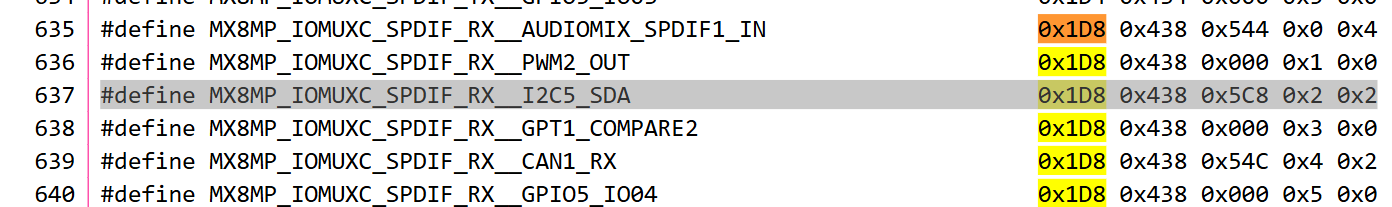
\includegraphics[width=0.75\linewidth]{mx8mp-pinfunc.h.png}
    \caption{mx8mp-pinfunc.h}
    \label{fig:placeholder}
\end{figure}
The \texttt{0x400001c3} pad control value sets:
\begin{itemize}
    \item Open-drain output (required for I2C)
    \item Pull-up enabled
    \item Hysteresis enabled
    \item Moderate drive strength
\end{itemize}

\subsection{Step 5: Add MPU-6050 Sensor Node}

Add the sensor as a child of the I2C5 controller:

\begin{lstlisting}[language=c]
&i2c5 {
    status = "okay";
    clock-frequency = <100000>;  // 100 kHz
    
    mpu6050@68 {
        compatible = "invensense,mpu6050";
        reg = <0x68>;              // I2C address (AD0 = LOW)
        // Use 0x69 if AD0 pin is HIGH
        
        status = "okay";
        
    };
};
\end{lstlisting}

\begin{important}
\textbf{Where do you find node schema?}

Check the kernel binding documentation:
\begin{itemize}
    \item \texttt{Documentation/devicetree/bindings/iio/imu/invensense,mpu6050.yaml}
\end{itemize}

In general, from what I've learnt yaml files lists all required and optional properties with examples. Just simply google <part you are looking for> yaml
\end{important}

\subsection{Step 6: Compile Modified Device Tree}

\begin{lstlisting}[language=bash]
# Compile DTS to DTB (with symbol preservation)
dtc -@ -I dts -O dtb \
    -o /tmp/imx8mp-evk-chyn.dtb \
    /tmp/imx8mp-evk-chyn.dts

# Copy to boot partition
cp /tmp/imx8mp-evk-chyn.dtb /run/media/boot-mmcblk2p1/

# Sync to ensure it's written
sync

# Verify it exists
ls -lh /run/media/boot-mmcblk2p1/imx8mp-evk-chyn.dtb
\end{lstlisting}

\subsection{Step 7: Configure U-Boot to Use New DTB}

\begin{lstlisting}[language=bash]
# Reboot and interrupt U-Boot
reboot

# In U-Boot console:
u-boot=> ls mmc 2:1
# Verify your .dtb file is present

u-boot=> setenv fdtfile imx8mp-evk-chyn.dtb
u-boot=> saveenv
Saving Environment to MMC... Writing to MMC(2)... OK

u-boot=> boot
\end{lstlisting}

\begin{important}
\textbf{Critical Step:} You MUST run \texttt{saveenv} to make the change permanent. Without it, the setting is lost on next reboot.
\end{important}

\subsection{Step 8: Verify Hardware Configuration}

After Linux boots, verify everything is configured correctly:

\textbf{A) Check device tree is loaded:}

\begin{lstlisting}[language=bash]
# Check I2C5 status
cat /proc/device-tree/soc@0/bus@30800000/i2c@30ad0000/status
okay

# Check sensor node exists
cat /proc/device-tree/soc@0/bus@30800000/i2c@30ad0000/mpu6050@68/compatible
invensense,mpu6050
\end{lstlisting}

\textbf{B) Verify pin muxing:}

\begin{lstlisting}[language=bash]
grep -E 'SPDIF_(TX|RX)|i2c5' /sys/kernel/debug/pinctrl/*/pinmux-pins

# Expected output:
pin 117 (MX8MP_IOMUXC_SPDIF_TX): 30ad0000.i2c (GPIO UNCLAIMED) function pinctrl group i2c5grp
pin 118 (MX8MP_IOMUXC_SPDIF_RX): 30ad0000.i2c (GPIO UNCLAIMED) function pinctrl group i2c5grp
\end{lstlisting}

\textbf{C) Check clocks are enabled:}

\begin{lstlisting}[language=bash]
cat /sys/kernel/debug/clk/clk_summary | grep -i i2c5

# Expected output:
i2c5                             0       0        0        24000000    0
   i2c5_root_clk                 0       0        0        24000000    0
\end{lstlisting}

\textbf{D) Scan I2C bus for device:}

\begin{lstlisting}[language=bash]
i2cdetect -y -r 4

# Expected output showing device at 0x68:
     0  1  2  3  4  5  6  7  8  9  a  b  c  d  e  f
00:                         -- -- -- -- -- -- -- --
10: -- -- -- -- -- -- -- -- -- -- -- -- -- -- -- --
20: -- -- -- -- -- -- -- -- -- -- -- -- -- -- -- --
30: -- -- -- -- -- -- -- -- -- -- -- -- -- -- -- --
40: -- -- -- -- -- -- -- -- -- -- -- -- -- -- -- --
50: -- -- -- -- -- -- -- -- -- -- -- -- -- -- -- --
60: -- -- -- -- -- -- -- -- 68 -- -- -- -- -- -- --
70: -- -- -- -- -- -- -- --
\end{lstlisting}

\textbf{E) Check driver binding:}

\begin{lstlisting}[language=bash]
# Load driver if built as module
modprobe inv_mpu6050_i2c

# Check driver loaded
ls -l /sys/bus/i2c/drivers/inv-mpu6050-i2c/

# Verify IIO device created
ls /sys/bus/iio/devices/

# Read sensor data
cat /sys/bus/iio/devices/iio:device0/in_accel_x_raw
cat /sys/bus/iio/devices/iio:device0/in_gyro_x_raw
\end{lstlisting}

If IIO device exists, your sensor is working!

\section{Common Device Tree Modifications}

\subsection{Disabling Unused Peripherals}

I think this is also a good start to learn how the device tree works, making small changes and seeing their corresponding results! To save power or free up pins, disable unused peripherals:

\begin{lstlisting}[language=c]
// Example: Disable FlexCAN (not using CAN bus)
&flexcan1 {
    status = "disabled";
};

&flexcan2 {
    status = "disabled";
};
\end{lstlisting}

After rebuilding and booting:
\begin{lstlisting}[language=bash]
# CAN0 should not appear
ip link show | grep can
# No output means CAN interfaces are disabled
\end{lstlisting}

\subsection{Changing I2C Bus Speed}

\begin{lstlisting}[language=c]
&i2c5 {
    clock-frequency = <400000>;  // 400 kHz (Fast Mode)
    // or <100000> for Standard Mode
    // or <1000000> for Fast Mode Plus
};
\end{lstlisting}

\subsection{Adding GPIO-Based Devices}

\begin{lstlisting}[language=c]
// Example: Add a GPIO LED
leds {
    compatible = "gpio-leds";
    
    status_led {
        label = "status:green";
        gpios = <&gpio5 3 GPIO_ACTIVE_HIGH>;
        default-state = "on";
    };
};
\end{lstlisting}


\section{Device Tree Overlays}

Overlays allow runtime modification of device tree without reflashing the entire DTB. However, this is advanced and not covered in this guide. For this internship, we modified the base DTS and recompiled.

\begin{docref}
\textbf{For device tree overlay usage:} See Linux kernel documentation:
\texttt{Documentation/devicetree/overlay-notes.rst}
\end{docref}

\section{Reference: i.MX8MP Device Tree Locations}

\subsection{Linux Kernel Source Structure}

\begin{verbatim}
linux/
|-- arch/
|   +-- arm64/
|       +-- boot/dts/
|           +-- freescale/
|               |-- imx8mp.dtsi           (SoC definitions)
|               |-- imx8mp-evk.dtsi       (EVK common)
|               |-- imx8mp-evk.dts        (Base board)
|               |-- imx8mp-evk-rpmsg.dts  (RPMsg variant)
|               +-- imx8mp-pinfunc.h      (Pin mux macros)
|
+-- include/
    +-- dt-bindings/
        |-- clock/
        |   +-- imx8mp-clock.h        (Clock indices)
        |-- interrupt-controller/
        |   +-- irq.h                 (IRQ flags)
        +-- gpio/
            +-- gpio.h                (GPIO flags)
\end{verbatim}

\subsection{Key Files to Reference}

\begin{itemize}
    \item \textbf{Pin functions:} \texttt{arch/arm64/boot/dts/freescale/imx8mp-pinfunc.h}
    \item \textbf{Clock indices:} \texttt{include/dt-bindings/clock/imx8mp-clock.h}
    \item \textbf{Binding docs:} \texttt{Documentation/devicetree/bindings/}
    \item \textbf{i.MX8MP Reference Manual:} Complete register map and peripheral descriptions
\end{itemize}


\subsection{Common Pitfalls}

\begin{important}
\textbf{Don't:}
\begin{itemize}
    \item Edit \texttt{.dtb} files directly - always work with \texttt{.dts}
    \item Forget to run \texttt{saveenv} in U-Boot
    \item Assume Linux bus numbers match hardware numbers (i2c-4 might be I2C5!)
    \item Skip verification steps - always check pinmux, clocks, and bus scan
    \item Modify SoC \texttt{.dtsi} files - override in board \texttt{.dts} instead
\end{itemize}
\end{important}

\chapter{Monitoring Infrastructure}

This chapter covers the complete monitoring setup used to track system performance, power consumption, and hardware state during development and testing. The monitoring stack consists of Zabbix for data collection and Grafana for visualization, both running in Docker containers on your development machine.

\textbf{Chapter organization:}
\begin{itemize}
    \item \textbf{Sections 6.1-6.9:} Setting up the monitoring infrastructure
    \item \textbf{Section 6.10:} Using the monitoring with stress testing (validation)
    \item \textbf{Section 6.11:} Summary and quick reference
\end{itemize}

\section{Why Monitoring is Essential}

\subsection{Purpose of This Setup}

During embedded system development, especially when working on power optimization, it will be nice to have  real-time visibility into:

\begin{itemize}
    \item \textbf{Power domain states} - Which parts of the SoC are on/off (GPU, VPU, NPU, audio)
    \item \textbf{CPU metrics} - Temperature, frequency, load per core
    \item \textbf{System resources} - Memory usage, I/O activity
    \item \textbf{Thermal behavior} - How the system heats up under load
    \item \textbf{Performance trends} - Historical data for benchmarking
\end{itemize}

\textbf{Use cases during my internship:}
\begin{itemize}
    \item Verify power domains turn off during idle (power optimization)
    \item Observe which components activate during specific workloads
    \item Measure impact of ATF modifications on power consumption
    \item Benchmark NPU/GPU performance under load
    \item Identify thermal throttling or anomalies
\end{itemize}



\section{Architecture Overview}
\begin{verbatim}
+---------------------------------------+
|   Development Laptop (Windows/WSL)    |
|                                       |
|   +-------------------------------+   |
|   |    Docker Containers          |   |
|   |                               |   |
|   |   +-------------+             |   |
|   |   | Zabbix      |             |   |
|   |   | Server      |             |   |
|   |   | (port 10051)|             |   |
|   |   +------+------+             |   |
|   |          |                    |   |
|   |          | Data storage       |   |
|   |          v                    |   |
|   |   +------+------+             |   |
|   |   | Grafana     |             |   |
|   |   | Dashboard   |             |   |
|   |   | (port 3000) |             |   |
|   |   +-------------+             |   |
|   |                               |   |
|   +-------------------------------+   |
|          ^                            |
+----------|----------------------------+
           |
           | TCP port 10051
           | (Zabbix data)
           | Ethernet
           |
+----------|----------------------------+
|          v                            |
|   i.MX8MP EVK Board                   |
|                                       |
|   +-------------------------------+   |
|   |   Zabbix Agent                |   |
|   |                               |   |
|   |   Collects & sends:           |   |
|   |   - Power domain states       |   |
|   |   - CPU temp/freq/load        |   |
|   |   - Memory usage              |   |
|   |   - Custom metrics            |   |
|   +-------------------------------+   |
|                                       |
+---------------------------------------+

Data Flow:
1. Zabbix Agent collects metrics from board
2. Sends to Zabbix Server (port 10051)
3. Zabbix stores data in internal database
4. Grafana queries Zabbix for visualization
5. You view dashboards at localhost:3000
\end{verbatim}


\subsection{Component Roles}

\begin{center}
\begin{tabular}{|l|p{9cm}|}
\hline
\textbf{Component} & \textbf{Purpose} \\
\hline
Zabbix Server & Collects and stores metrics, triggers alerts \\
\hline
Zabbix Agent & Runs on i.MX8MP, gathers system metrics \\
\hline
Grafana & Visualizes data with customizable dashboards \\
\hline
PostgreSQL & Database backend for Zabbix (in Docker) \\
\hline
Docker Compose & Orchestrates all containers on laptop \\
\hline
\end{tabular}
\end{center}

\section{Prerequisites}

\subsection{Network Requirements}

\begin{important}
\textbf{Critical:} Both laptop and i.MX8MP board must be on the same network. At DSO, I used Ethernet connection via router .
\end{important}

\textbf{Check IP addresses:}

On i.MX8MP board:
\begin{lstlisting}[language=bash]
root@imx8mp-lpddr4-evk:~# ip a
# Look for inet address on eth0, e.g., 192.168.1.100
\end{lstlisting}

On laptop (Windows):
\begin{lstlisting}[language=bash]
ipconfig
# Look for Ethernet adapter IP, e.g., 192.168.1.50
\end{lstlisting}

Both should be in the same subnet (e.g., 192.168.1.x).

\subsection{Software Requirements}

\textbf{On development laptop:}
\begin{itemize}
    \item Docker Desktop installed and running
    \item Docker Compose (included with Docker Desktop)
\end{itemize}

\textbf{On i.MX8MP board:}
\begin{itemize}
    \item Zabbix agent package (added via Yocto - see Chapter 4)
    \item Root or sudo access for power domain monitoring
\end{itemize}

\section{Docker Setup (Laptop/Host)}

\subsection{Prerequisites: Docker Installation}

\begin{docref}
\textbf{Docker Desktop Setup:}

Before proceeding, ensure Docker Desktop is properly installed and running on your laptop. For DSO-specific Docker installation procedures, refer to:

\textbf{github Bases  IT Service  "Docker Desktop Installation and Configuration"}

\textbf{Verify Docker is working:}
\begin{lstlisting}[language=bash]
docker --version
docker-compose --version
docker ps  # Should run without errors
\end{lstlisting}
\end{docref}

\subsection{Configuration Files Repository}

\begin{gitref}
\textbf{All Monitoring Configuration Files:}

The complete docker-compose.yml and all configuration files are available at:

\url{https://github.com/yulyuri/firmware-and-dts/tree/master/zabbixgrafanastuff/zabbix-dso}

\textbf{Directory structure:}
\begin{verbatim}
monitoring/
|-- docker-compose.yml           <- Start here
|-- zabbix_agentd.conf          <- Board agent config
|-- custom_metrics.conf          <- Power domain metrics
+-- grafana-dashboard.json       <- Pre-built dashboard
\end{verbatim}

\textbf{Quick start:} Clone the folder and use the provided files instead of creating from scratch. The Grafana dashboard JSON can be imported directly to get the complete power monitoring setup instantly.
\end{gitref}

\subsection{Create Project Directory}

\begin{lstlisting}[language=bash]
# On Windows with WSL2 or Linux:
mkdir -p ~/Desktop/zabbix-dso
cd ~/Desktop/zabbix-dso
\end{lstlisting}

\subsection{Docker Compose Configuration}

Create \texttt{docker-compose.yml} in the project directory or just download from github:

\begin{lstlisting}[language=yaml]
version: "3.8"
services:
  zabbix:
    image: zabbix/zabbix-appliance:alpine-latest
    container_name: zabbix-1
    ports:
      - "8080:80"       # Zabbix frontend
      - "10051:10051"   # Zabbix server
    networks:
      - zbxnet
      
  zabbix-agent:
    image: zabbix/zabbix-agent:alpine-latest
    container_name: zabbix-agent-1
    environment:
      - ZBX_SERVER_HOST=zabbix-1
      - ZBX_HOSTNAME=zabbix-agent-1
    networks:
      - zbxnet
      
  grafana:
    image: grafana/grafana:latest
    container_name: grafana-1
    ports:
      - "3000:3000"
    networks:
      - zbxnet
      
networks:
  zbxnet:
    driver: bridge
\end{lstlisting}

\begin{important}
\textbf{About This Setup:}

\textbf{zabbix-appliance:} This is an all-in-one image that includes:
\begin{itemize}
    \item Zabbix Server
    \item Zabbix Frontend (web UI)
    \item MySQL database (internal) - stores all metrics and configuration
    \item All bundled together for easy deployment
\end{itemize}

This simplifies setup significantly compared to running separate database, server, and frontend containers.

\textbf{zabbix-agent container:} This container is included in the compose file but not actually used. The real Zabbix agent runs directly on the i.MX8MP board, not in Docker.

\textbf{grafana:} Visualization and dashboard platform that queries Zabbix for data.
\end{important}

\subsection{Start Docker Containers}

\begin{lstlisting}[language=bash]
cd ~/Desktop/zabbix-dso

# Start all containers in background
docker-compose up -d

# Verify all containers are running
docker ps

# Expected output: 3 containers running
# - zabbix-1
# - zabbix-agent-1 (not used, but running)
# - grafana-1
\end{lstlisting}

\textbf{Check container logs if issues:}
\begin{lstlisting}[language=bash]
docker-compose logs zabbix
docker-compose logs grafana
\end{lstlisting}

\subsection{Access Web Interfaces}

\textbf{Zabbix Web UI:}
\begin{itemize}
    \item URL: \url{http://localhost:8080}
    \item Default username: \texttt{Admin}
    \item Default password: \texttt{zabbix}
\end{itemize}

\textbf{Grafana:}
\begin{itemize}
    \item URL: \url{http://localhost:3000}
    \item Default username: \texttt{admin}
    \item Default password: \texttt{admin} 
\end{itemize}

\begin{important}
\textbf{First time setup:} Docker will download images (~1-2 GB). This takes a few minutes. Subsequent starts are instant.
\end{important}

\subsection{Future Work: External Database}

\begin{important}
\textbf{Current Limitation:}

The zabbix-appliance uses an internal MySQL database for storing all metrics and configuration. This is sufficient for development and testing but has limitations:

\textbf{Limitations:}
\begin{itemize}
    \item Data is stored inside the container (will belost if container gone)
    \item Limited scalability for long-term data retention
    \item No easy backup/restore mechanism
    \item Can't share database with other services
\end{itemize}

\textbf{Possible Future Improvement:}

Set up an external database (I was exploring InfluxDB) to:
\begin{itemize}
    \item Persist data outside containers (process/view data after)
    \item Enable long-term historical analysis (days of data)
    \item Implement proper backup strategies
    \item Scale storage independently from Zabbix server
    \item Share data with other analysis tools
\end{itemize}

\textbf{This was not completed during my internship} but I think would be useful down the road when everything is set up (PX4 code etc) and can be used for more comprehensive platform for development, testing, and monitoring.
\end{important}

\section{Zabbix Agent Setup (i.MX8MP Board)}

\subsection{Verify Zabbix Agent Installation}

Zabbix agent should already be installed if you added it to your Yocto build (Chapter 4).

\begin{lstlisting}[language=bash]
# Check if zabbix agent is installed
root@imx8mp-lpddr4-evk:~# which zabbix_agentd
/usr/sbin/zabbix_agentd

# Check version
root@imx8mp-lpddr4-evk:~# zabbix_agentd --version
zabbix_agentd (daemon) (Zabbix) 7.0.9
\end{lstlisting}

If not installed, you need to rebuild your Yocto image with zabbix package (see Chapter 4).

\subsection{Configure Zabbix Agent}

Edit the main configuration file:

\begin{lstlisting}[language=bash]
nano /etc/zabbix/zabbix_agentd.conf
\end{lstlisting}

\textbf{Key settings to change:}

\begin{lstlisting}[language=bash]
# Server IP (your laptop's IP address)
Server=192.168.1.50

# Active checks (send data to server)
ServerActive=192.168.1.50:10051

# Hostname (must match in Zabbix web UI later)
Hostname=imx8mp-board

# Allow root to run commands (needed for power domain access)
AllowRoot=1

# Include custom metrics directory
Include=/etc/zabbix/zabbix_agentd.conf.d/*.conf
\end{lstlisting}

\begin{important}
Replace \texttt{192.168.1.50} with your actual laptop IP address!
\end{important}

\subsection{Create Custom Metrics Configuration}

Create directory and configuration file for custom metrics:

\begin{lstlisting}[language=bash]
mkdir -p /etc/zabbix/zabbix_agentd.conf.d
nano /etc/zabbix/zabbix_agentd.conf.d/custom_metrics.conf

this conf file might be in /etc/zabbix_agentd.conf as well. please check properly.
\end{lstlisting}

Add the following UserParameter definitions:

\begin{lstlisting}[language=bash]
# CPU Metrics
UserParameter=cpu.temp,awk '{printf "%.1f", $1/1000}' /sys/class/thermal/thermal_zone0/temp
UserParameter=cpu.freq,awk '{printf "%.0f", $1/1000}' /sys/devices/system/cpu/cpu0/cpufreq/scaling_cur_freq
UserParameter=cpu0.usage,awk '/^cpu0 / {u=$2+$3+$4; t=$2+$3+$4+$5+$6+$7+$8; print int((u/t)*100)}' /proc/stat

# System Metrics
UserParameter=load.1min,cut -d' ' -f1 /proc/loadavg
UserParameter=mem.free,free -m | awk '/Mem:/ {print $4}'

# Power Domain States (on=1, off=0)
UserParameter=power.gpu3d,grep -q on /sys/kernel/debug/pm_genpd/gpu3d/current_state && echo 1 || echo 0
UserParameter=power.gpu2d,grep -q on /sys/kernel/debug/pm_genpd/gpu2d/current_state && echo 1 || echo 0
UserParameter=power.vpumix,grep -q on /sys/kernel/debug/pm_genpd/vpumix/current_state && echo 1 || echo 0
UserParameter=power.vpu-g1,grep -q on /sys/kernel/debug/pm_genpd/vpu-g1/current_state && echo 1 || echo 0
UserParameter=power.vpu-g2,grep -q on /sys/kernel/debug/pm_genpd/vpu-g2/current_state && echo 1 || echo 0
UserParameter=power.mlmix,grep -q on /sys/kernel/debug/pm_genpd/mlmix/current_state && echo 1 || echo 0
UserParameter=power.audiomix,grep -q on /sys/kernel/debug/pm_genpd/audiomix/current_state && echo 1 || echo 0
\end{lstlisting}



\subsection{Start Zabbix Agent}

\begin{lstlisting}[language=bash]
# Start agent manually (for testing)
zabbix_agentd -c /etc/zabbix/zabbix_agentd.conf

# Or use systemd (if configured)
systemctl restart zabbix-agent
systemctl status zabbix-agent
\end{lstlisting}

\subsection{Test Custom Metrics}

Verify that custom metrics work:

\begin{lstlisting}[language=bash]
# Test individual metrics
zabbix_agentd -t cpu.temp
# Expected: cpu.temp [t|45.2]

zabbix_agentd -t power.gpu3d
# Expected: power.gpu3d [t|0] or [t|1]

zabbix_agentd -t mem.free
# Expected: mem.free [t|1234]
\end{lstlisting}

\textbf{Common errors:}
\begin{itemize}
    \item \texttt{[m|ZBX\_NOTSUPPORTED] [Unsupported item key.]} - Metric not defined in config
    \item \texttt{[m|ZBX\_NOTSUPPORTED] [Cannot obtain system information.]} - Permission denied or path wrong
    \item No output - Agent not running or config file not loaded
\end{itemize}

\section{Power Domain Monitoring Deep Dive}

\subsection{What Are Power Domains?}

The i.MX8M Plus has multiple power domains that can be independently controlled to save power:

\begin{center}
\begin{tabular}{|l|p{8cm}|}
\hline
\textbf{Domain} & \textbf{Controls} \\
\hline
gpu3d & 3D graphics accelerator \\
\hline
gpu2d & 2D graphics and compositor \\
\hline
vpumix & Video processing unit parent domain \\
\hline
vpu-g1 & VPU decoder (H.264, etc.) \\
\hline
vpu-g2 & VPU encoder/decoder (HEVC, VP9) \\
\hline
mlmix & Machine learning accelerator (NPU) \\
\hline
audiomix & Audio processing and codecs \\
\hline
\end{tabular}
\end{center}

\subsection{Power State Files}

Linux exposes power domain states via debugfs:

\begin{lstlisting}[language=bash]
# Check all power domain states
root@imx8mp-lpddr4-evk:~# ls /sys/kernel/debug/pm_genpd/
audiomix  gpu2d  gpu3d  mlmix  vpu-g1  vpu-g2  vpumix

# Check individual state
root@imx8mp-lpddr4-evk:~# cat /sys/kernel/debug/pm_genpd/gpu3d/current_state
off

# When GPU is active:
root@imx8mp-lpddr4-evk:~# cat /sys/kernel/debug/pm_genpd/gpu3d/current_state
on
\end{lstlisting}

\subsection{Why This Matters}

\textbf{For power optimization:}
\begin{itemize}
    \item Idle domains should be OFF to save power
    \item Monitoring shows if optimizations actually work
    \item Can identify "zombie" domains that stay on unnecessarily
\end{itemize}

\textbf{For debugging:}
\begin{itemize}
    \item See which workload activates which domain
    \item Verify driver power management is working
    \item Understand system behavior under different loads
\end{itemize}

\begin{important}
\textbf{Example Discovery:} During testing, you might notice \texttt{audiomix} stays on even when not playing audio. This indicates a potential driver bug or missing power management hook - something you'd never discover without monitoring!
\end{important}

\section{Zabbix Web UI Configuration}

\subsection{Add Host (i.MX8MP Board)}

\begin{enumerate}
    \item Log into Zabbix: \url{http://localhost:8080}
    \item Go to: \textbf{Configuration → Hosts}
    \item Click \textbf{Create host}
    \item Fill in:
    \begin{itemize}
        \item \textbf{Host name:} \texttt{imx8mp-board} (must match agent config!)
        \item \textbf{Groups:} Select "Linux servers" or create "Embedded Devices"
        \item \textbf{Agent interface:} Add IP address of i.MX8MP (e.g., 192.168.1.100)
        \item \textbf{Port:} 10050
    \end{itemize}
    \item Click \textbf{Add}
\end{enumerate}

\textbf{Verify connection:}
\begin{itemize}
    \item Go to \textbf{Monitoring → Latest data}
    \item Select host: \texttt{imx8mp-board}
    \item Should see "ZBX" indicator turn green within 60 seconds
\end{itemize}

\subsection{Create Custom Items}

For each custom metric, create an item:

\begin{enumerate}
    \item Go to: \textbf{Configuration → Hosts → imx8mp-board → Items}
    \item Click \textbf{Create item}
    \item For GPU3D power state:
    \begin{itemize}
        \item \textbf{Name:} GPU3D Power State
        \item \textbf{Key:} \texttt{power.gpu3d}
        \item \textbf{Type of information:} Numeric (unsigned)
        \item \textbf{Update interval:} 5s
    \end{itemize}
    \item Repeat for all power domains and metrics
\end{enumerate}


\section{Grafana Dashboard Setup}

\subsection{Install Zabbix Plugin}

\begin{enumerate}
    \item Access Grafana: \url{http://localhost:3000}
    \item Go to: \textbf{Administration → Plugins}
    \item Search for: \textbf{Zabbix}
    \item Install: \textbf{Zabbix plugin by Alexander Zobnin}
\end{enumerate}

\textbf{Note:} The Docker Compose file already installs this plugin, so it should be available.

\subsection{Add Zabbix Data Source}

\begin{enumerate}
    \item Go to: \textbf{Connections → Data sources}
    \item Click \textbf{Add data source}
    \item Select \textbf{Zabbix}
    \item Configure:
    \begin{itemize}
        \item \textbf{Name:} Zabbix Server
        \item \textbf{URL:} \texttt{http://zabbix-server:8080/api\_jsonrpc.php}
        \item \textbf{Username:} Admin
        \item \textbf{Password:} zabbix
    \end{itemize}
    \item Click \textbf{Save \& Test}
    \item Should show: "Data source is working"
\end{enumerate}



\subsection{Create Power Domain Dashboard}

\begin{enumerate}
    \item Go to: \textbf{Dashboards → New → New Dashboard}
    \item Click \textbf{Add visualization}
    \item Select \textbf{Polystat} panel
    \item Configure panel:
    \begin{itemize}
        \item \textbf{Data source:} Zabbix Server
        \item \textbf{Group:} Embedded Devices (or your host group)
        \item \textbf{Host:} imx8mp-board
        \item \textbf{Item:} power.gpu3d
    \end{itemize}
    \item Under \textbf{Polystat options:}
    \begin{itemize}
        \item \textbf{Layout:} Honeycomb or AutoSize
        \item \textbf{Color mode:} Threshold-based
        \item \textbf{Thresholds:}
        \begin{itemize}
            \item 0 = Red (domain OFF)
            \item 1 = Green (domain ON)
        \end{itemize}
    \end{itemize}
    \item Click \textbf{Apply}
    \item Repeat for other power domains
\end{enumerate}

\textbf{Organize panels by rows:}
\begin{itemize}
    \item Row 1: GPU domains (gpu3d, gpu2d)
    \item Row 2: VPU domains (vpumix, vpu-g1, vpu-g2)
    \item Row 3: Other domains (mlmix, audiomix)
\end{itemize}

\subsection{Add System Metrics Panels}

\textbf{CPU Temperature (Gauge):}
\begin{itemize}
    \item Panel type: Gauge
    \item Item: cpu.temp
    \item Min: 20, Max: 90
    \item Thresholds: Green <60, Yellow 60-75, Red >75
\end{itemize}

\textbf{Memory Free (Stat):}
\begin{itemize}
    \item Panel type: Stat
    \item Item: mem.free
    \item Unit: MB
\end{itemize}

\textbf{Load Average (Graph):}
\begin{itemize}
    \item Panel type: Time series
    \item Item: load.1min
    \item Shows system load over time
\end{itemize}
\begin{figure}[H]
    \centering
    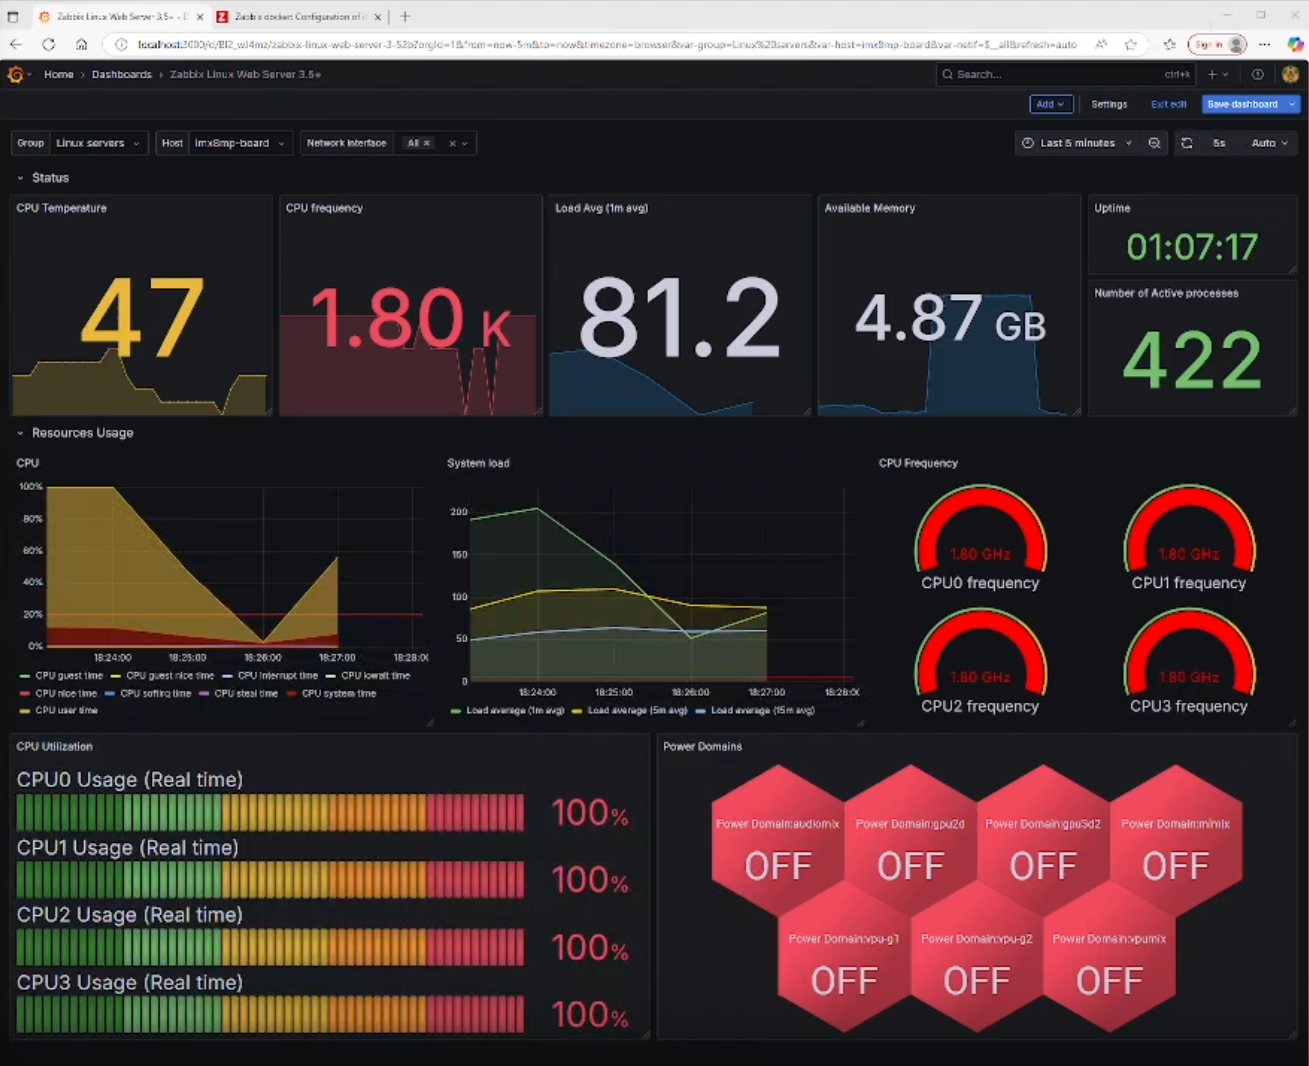
\includegraphics[width=0.75\linewidth]{grafana.png}
    \caption{Grafana Dashboard}
    \label{fig:placeholder}
\end{figure}
% TODO: Add screenshots of complete dashboard


\section{System Validation with Stress Testing}

\begin{important}
\textbf{Important Distinction:}

The following sections describe how to \textbf{USE} the monitoring infrastructure you just set up. stress-ng is \textbf{NOT part of the monitoring stack} - it's a separate testing tool that generates controlled load so you can observe system behavior through Zabbix and Grafana.

\textbf{Workflow:}
\begin{enumerate}
    \item Open Grafana dashboard (monitoring is already running)
    \item Run stress-ng on the i.MX8MP board (generates load)
    \item Watch power domains, temperature, CPU frequency change in real-time on Grafana
    \item Document findings and validate optimizations
\end{enumerate}
\end{important}


\subsection{What is stress-ng?}

\texttt{stress-ng} (stress next generation) is a comprehensive Linux system stress testing tool that can exercise various subsystems including CPU, memory, I/O, filesystem, and more.

\textbf{Key capabilities:}
\begin{itemize}
    \item 280+ different stress test methods
    \item Parallel execution of multiple stressors
    \item Configurable duration and intensity
    \item Built-in metrics and verification
    \item Minimal dependencies (works on embedded systems)
\end{itemize}

\begin{docref}
\textbf{Complete stress-ng Documentation:}

\begin{itemize}
    \item GitHub repository: \url{https://github.com/ColinIanKing/stress-ng}
    \item Manual page: \url{https://manpages.ubuntu.com/manpages/jammy/man1/stress-ng.1.html}
    \item Stress methods reference: \url{https://wiki.ubuntu.com/Kernel/Reference/stress-ng}
\end{itemize}

These resources document all available stress tests, options, and usage examples.
\end{docref}

\subsection{Installation}

\textbf{Recommended: Add to Yocto build}

\begin{lstlisting}[language=bash]
# In build-xwayland/conf/local.conf
IMAGE_INSTALL:append = " stress-ng"

# Rebuild image
bitbake imx-image-full
\end{lstlisting}

\textbf{Verify installation:}
\begin{lstlisting}[language=bash]
root@imx8mp-lpddr4-evk:~# stress-ng --version
stress-ng, version 0.XX.XX
\end{lstlisting}

\subsection{Stress Testing Commands}

\textbf{CPU stress (all cores):}
\begin{lstlisting}[language=bash]
stress-ng --cpu 4 --timeout 60s
\end{lstlisting}

\textbf{Memory stress:}
\begin{lstlisting}[language=bash]
stress-ng --vm 2 --vm-bytes 512M --timeout 60s
\end{lstlisting}

\textbf{I/O stress:}
\begin{lstlisting}[language=bash]
stress-ng --io 2 --hdd 1 --timeout 60s
\end{lstlisting}

\textbf{Comprehensive stress (all-in-one):}
\begin{lstlisting}[language=bash]
stress-ng --cpu 4 --io 2 --vm 2 --hdd 1 --timeout 120s
\end{lstlisting}

\textbf{CPU method variations:}
\begin{lstlisting}[language=bash]
# Test all CPU stress methods
stress-ng --cpu 4 --cpu-method all --timeout 60s

# Specific methods
stress-ng --cpu 4 --cpu-method fft --timeout 60s
stress-ng --cpu 4 --cpu-method matrixprod --timeout 60s
\end{lstlisting}

\subsection{Stress Test Categories}

stress-ng organizes tests into categories based on what subsystem they stress:

\textbf{CPU stressors:}
\begin{lstlisting}[language=bash]
# Integer arithmetic
stress-ng --cpu 4 --cpu-method ackermann --timeout 60s

# Floating point operations
stress-ng --cpu 4 --cpu-method fft --timeout 60s
stress-ng --cpu 4 --cpu-method omega --timeout 60s

# Matrix operations
stress-ng --cpu 4 --cpu-method matrixprod --timeout 60s

# All CPU methods sequentially
stress-ng --cpu 4 --cpu-method all --timeout 300s
\end{lstlisting}

\textbf{Memory stressors:}
\begin{lstlisting}[language=bash]
# Virtual memory allocation/deallocation
stress-ng --vm 2 --vm-bytes 512M --timeout 60s

# Memory copy operations
stress-ng --memcpy 4 --timeout 60s

# Cache thrashing
stress-ng --cache 4 --timeout 60s

# Memory bandwidth stress
stress-ng --stream 4 --timeout 60s
\end{lstlisting}

\textbf{I/O and filesystem stressors:}
\begin{lstlisting}[language=bash]
# Generic I/O operations
stress-ng --io 4 --timeout 60s

# Disk write/read
stress-ng --hdd 2 --hdd-bytes 256M --timeout 60s

# File allocation
stress-ng --fallocate 4 --timeout 60s

# Directory operations
stress-ng --dentry 4 --timeout 60s
\end{lstlisting}


\subsection{Useful stress-ng Options}

\begin{center}
\begin{tabular}{|l|p{7cm}|}
\hline
\textbf{Option} & \textbf{Purpose} \\
\hline
--timeout Ns & Run for N seconds \\
\hline
--metrics & Show bogo ops (operations/sec) at end \\
\hline
--metrics-brief & Condensed metrics output \\
\hline
--verify & Verify computations are correct \\
\hline
--log-file FILE & Save output to file for later analysis \\
\hline
--aggressive & More intense stress (higher resource usage) \\
\hline
--taskset N & Pin workers to specific CPU cores \\
\hline
--cpu-load N\% & Target N\% CPU load (vs 100\%) \\
\hline
\end{tabular}
\end{center}

\textbf{Example with metrics:}
\begin{lstlisting}[language=bash]
stress-ng --cpu 4 --timeout 60s --metrics-brief
# Shows: bogo ops/s for each worker (performance metric)
\end{lstlisting}

\textbf{Pin to specific cores:}
\begin{lstlisting}[language=bash]
# Stress only cores 0 and 1
stress-ng --cpu 2 --taskset 0,1 --timeout 60s

# Test single core performance
stress-ng --cpu 1 --taskset 0 --timeout 60s
\end{lstlisting}

\subsection{Thermal Behavior Observations}

\begin{important}
\textbf{Key Finding from Extended Stress Testing:}

During comprehensive stress testing over extended periods (60+ seconds with maximum load), the following thermal behavior was consistently observed:

\textbf{Temperature Profile:}
\begin{itemize}
    \item \textbf{Idle:} 35-40°C
    \item \textbf{Light load (1-2 cores):} 45-50°C
    \item \textbf{Heavy load (all cores):} 55-60°C
    \item \textbf{Peak temperature:} \textbf{Never exceeded 60°C}
    \item \textbf{Thermal throttling:} \textbf{Never observed}
\end{itemize}

\textbf{Implications:}
\begin{itemize}
    \item The EVK board has adequate cooling (heatsink + natural airflow)
    \item The i.MX8MP's thermal design is conservative
    \item No thermal throttling interferes with benchmarking results
    \item The board can sustain full CPU load indefinitely
    \item Temperature is not a limiting factor for performance testing
\end{itemize}


\end{important}


\subsection{What could be explored next: CPU Frequency Scaling and Governors}

During this internship, CPU frequency scaling was observed but not thoroughly investigated. This is an important area for future work, especially for real-time flight control applications.

\subsubsection{Current Status}

The i.MX8MP uses the Linux CPUfreq framework to dynamically scale CPU frequency based on load. The system was tested with the default governor, but detailed characterization of scaling behavior was not completed.

\textbf{Check current configuration:}
\begin{lstlisting}[language=bash]
# Current governor
cat /sys/devices/system/cpu/cpu0/cpufreq/scaling_governor
# ondemand , performance etc

# Current frequency for each core
cat /sys/devices/system/cpu/cpu*/cpufreq/scaling_cur_freq
# Shows frequency in kHz (e.g., 1800000 = 1.8 GHz)

# Min/Max frequency limits
cat /sys/devices/system/cpu/cpu0/cpufreq/scaling_min_freq
cat /sys/devices/system/cpu/cpu0/cpufreq/scaling_max_freq

# Available frequency steps
cat /sys/devices/system/cpu/cpu0/cpufreq/scaling_available_frequencies
\end{lstlisting}

\textbf{Monitor frequency in real-time:}
\begin{lstlisting}[language=bash]
# Watch all cores
watch -n 0.5 'cat /sys/devices/system/cpu/cpu*/cpufreq/scaling_cur_freq'

# Or use Grafana (if cpu.freq metric configured)
# More convenient for observing during stress tests
\end{lstlisting}

\subsubsection{Unexplored Questions}

\begin{important}
\textbf{Critical Questions for Future Investigation:}

\textbf{Governor Behavior (Thresholds and Timing):}
\begin{itemize}
    \item At what CPU utilization percentage does the governor trigger frequency up-scaling?
    \item How long does the CPU stay at high frequency before scaling down?
    \item What is the time window for calculating "load"? (1ms? 10ms? 100ms?)
    \item Is load calculated per-core or system-wide?
    \item Does the governor consider thermal feedback when scaling?
    \item What happens when a high-priority real-time task wakes up? Immediate scaling or delayed?
\end{itemize}

\textbf{Governor Comparison (Performance vs Power):}
\begin{itemize}
    \item \textbf{Performance impact:} How much faster is "performance" vs "schedutil" for typical workloads?
    \item \textbf{Power consumption:} Measure actual power draw differences between governors
    \item \textbf{Latency:} Time to scale from minimum to maximum frequency
    \item \textbf{Response time:} How quickly does governor react to load changes?
    \item \textbf{Best for flight control:} Which governor provides lowest latency for real-time tasks?
\end{itemize}

\textbf{Scaling Parameters (Tuning Potential):}
\begin{itemize}
    \item Can up-scaling thresholds be adjusted? (e.g., scale up at 70\% load instead of 80\%)
    \item Can down-scaling delay be configured? (stay at high freq longer)
    \item Are there governor-specific tunables in \texttt{/sys/devices/system/cpu/cpufreq/}?
    \item What's the overhead of frequency transitions themselves?
\end{itemize}
\end{important}

\subsubsection{Quick Governor Switching for Testing}

\begin{lstlisting}[language=bash]
# Switch to performance governor (fixed maximum frequency)
echo performance | sudo tee /sys/devices/system/cpu/cpu*/cpufreq/scaling_governor

# Switch to powersave governor (fixed minimum frequency)
echo powersave | sudo tee /sys/devices/system/cpu/cpu*/cpufreq/scaling_governor

# Switch to schedutil (dynamic, scheduler-driven - recommended)
echo schedutil | sudo tee /sys/devices/system/cpu/cpu*/cpufreq/scaling_governor

# Switch to ondemand (dynamic, legacy but common)
echo ondemand | sudo tee /sys/devices/system/cpu/cpu*/cpufreq/scaling_governor

# Verify change took effect
cat /sys/devices/system/cpu/cpu0/cpufreq/scaling_governor
\end{lstlisting}

\textbf{Suggested testing procedure:}
\begin{enumerate}
    \item Switch to performance governor
    \item Run stress-ng benchmark, record metrics
    \item Switch to powersave governor
    \item Run same benchmark, record metrics (will be much slower!)
    \item Switch to schedutil governor
    \item Run same benchmark, record metrics
    \item Compare: performance, power consumption (if measurable), temperature
    \item Observe frequency changes in Grafana during each test
\end{enumerate}

\begin{docref}
\textbf{Recommended Tools for Deep Governor Investigation:}

\begin{itemize}
    \item \textbf{trace-cmd / ftrace:} Kernel tracing to capture frequency transitions with timestamps
    \item \textbf{perf:} CPU performance counter analysis
    \item \textbf{powertop:} Power consumption analysis tool
    \item \textbf{schedviz:} Visualize scheduler behavior and frequency changes
\end{itemize}

Example trace command:
\begin{lstlisting}[language=bash]
# Trace frequency changes
trace-cmd record -e power:cpu_frequency -e sched:sched_switch
trace-cmd report
\end{lstlisting}
\end{docref}

\subsubsection{Implications for Flight Control}

For PX4 flight controller software (Chapter 9: M7 Development), CPU frequency scaling behavior is critical:

\begin{itemize}
    \item \textbf{Latency sensitivity:} Flight control requires deterministic response times
    \item \textbf{Real-time performance:} Frequency scaling can introduce jitter
    \item \textbf{Power efficiency:} Lower frequencies save power during hover/cruise
    \item \textbf{Recommendation:} May need to pin flight control threads to specific cores at fixed frequency
\end{itemize}

This investigation should be completed before deploying any flight control software.

\subsection{Other Unexplored Monitoring Topics}

\subsubsection{Database Integration}

As mentioned earlier, migrating to an external database would enable:
\begin{itemize}
    \item InfluxDB for time-series data (better than MySQL for metrics)
    \item Long-term trend analysis (weeks/months of data)
    \item Automated anomaly detection
    \item Machine learning on historical data
\end{itemize}

\subsubsection{Additional Power Domains}

Other power domains exist but were not monitored:
\begin{itemize}
    \item HDMI/MIPI display power domains
    \item PCIe power management states
    \item USB subsystem power states
    \item SATA/storage power management
\end{itemize}

Check availability: \texttt{ls /sys/kernel/debug/pm\_genpd/}

\subsubsection{Per-Core Metrics}

More granular CPU monitoring:
\begin{itemize}
    \item Individual core frequency tracking (each core independently)
    \item some sort of more accurate way to measure temperature? other than thermal zones?
    \item Core isolation testing (disable cores, test performance)
    \item CPU affinity impact on performance
\end{itemize}

\subsubsection{Advanced Grafana Dashboards/graphs/visualisation}

Potential dashboard improvements:
\begin{itemize}
    \item Correlation panels (show CPU load vs frequency vs temperature)
    \item Comparison views (before/after optimization side-by-side)
    \item Annotations for test events (mark when tests started/ended)
\end{itemize}

\section{Startup Procedure (Quick Reference)}

\subsection{Every Time You Start Monitoring}

\textbf{Step 1: Start Docker containers (Laptop)}
\begin{lstlisting}[language=bash]
cd ~/Desktop/zabbix-dso
docker-compose up -d
docker ps  # Verify all running
\end{lstlisting}

\textbf{Step 2: Get board IP address}
\begin{lstlisting}[language=bash]
# On i.MX8MP
ip a
# Note the IP, e.g., 192.168.1.100
\end{lstlisting}

\textbf{Step 3: Update Zabbix agent config (if IP changed)}
\begin{lstlisting}[language=bash]
# Only if laptop IP changed
nano /etc/zabbix/zabbix_agentd.conf
# Update Server= and ServerActive= lines
\end{lstlisting}

\textbf{Step 4: Start Zabbix agent (Board)}
\begin{lstlisting}[language=bash]
zabbix_agentd -c /etc/zabbix/zabbix_agentd.conf
# Or: systemctl restart zabbix-agent
\end{lstlisting}

\textbf{Step 5: Access dashboards}
\begin{itemize}
    \item Zabbix: \url{http://localhost:8080}
    \item Grafana: \url{http://localhost:3000}
\end{itemize}

\chapter{NPU and Machine Learning}

\begin{important}
\textbf{Exploration Status:}

This chapter documents preliminary NPU exploration conducted over approximately \textbf{one day} of testing. The work focused on:
\begin{itemize}
    \item Verifying NPU functionality with basic inference
    \item Understanding TensorFlow Lite with VX Delegate
    \item Running benchmark models (MobileNet V1)
    \item Basic performance profiling
\end{itemize}

\textbf{This is NOT comprehensive ML optimization work.} There is significant room for exploration in quantization strategies, model optimization, and understanding what computer vision tasks are actually required for guided systems/drone applications.
\end{important}

\section{Introduction}

\subsection{Why NPU Matters for Embedded Systems}

The i.MX8M Plus includes a dedicated Neural Processing Unit (NPU) capable of 2.3 TOPS (Tera Operations Per Second) for AI inference. This hardware accelerator enables:

\begin{itemize}
    \item \textbf{Real-time computer vision} - Object detection, tracking
    \item \textbf{Low power inference} - More efficient than CPU/GPU
    \item \textbf{Parallel processing} - Optimized for neural network operations
    \item \textbf{Edge AI} - Run models locally without cloud dependency
\end{itemize}

\textbf{Potential applications for drone/guided systems:}
\begin{itemize}
    \item Object detection and avoidance
    \item Target tracking and recognition
    \item Autonomous navigation
    \item Visual odometry
    \item Situational awareness
\end{itemize}

\begin{hardware}
\textbf{i.MX8MP NPU Specifications:}
\begin{itemize}
    \item \textbf{Architecture:} Vivante VIP8000NanoSi-UltraLite
    \item \textbf{Performance:} 2.3 TOPS INT8
    \item \textbf{Power:} Integrated with automatic power management
    \item \textbf{Frameworks:} TensorFlow Lite, ONNX Runtime (via delegates)
    \item \textbf{Quantization:} Optimized for INT8, supports mixed precision
\end{itemize}
\end{hardware}

\subsection{Scope of This Investigation}

During this internship, NPU work was limited to:
\begin{enumerate}
    \item Basic setting up of TensorFlow Lite runtime
    \item Understanding VX Delegate (NPU acceleration layer)
    \item Running pre-trained quantized models
    \item Basic performance benchmarking
    \item Exploring profiling tools
\end{enumerate}

\textbf{What was NOT explored:}
\begin{itemize}
    \item Custom model training and optimization
    \item Quantization strategy comparison (INT8 vs mixed precision)
    \item Real-world application development (object detection pipeline)
    \item Power consumption measurement during inference
    \item Integration with flight control software
    \item What CV tasks are actually needed for DSO's guided systems
    \item How to use it concurrently with other tasks? What kind of ML tasks should be offloaded to NPU etc. 
\end{itemize}

\section{NPU Architecture and Power Management}

\subsection{What is a Delegate?}

A \textbf{delegate} is a plugin or runtime module that tells the inference engine \textbf{how} and \textbf{where} to execute a model.

\textbf{Common delegates:}
\begin{itemize}
    \item \textbf{Default (no delegate):} Runs on CPU using optimized kernels
    \item \textbf{GPU Delegate:} Offloads operations to GPU
    \item \textbf{VX Delegate (libvx\_delegate.so):} Offloads to NPU on i.MX8MP
    \item \textbf{XNNPACK:} Highly optimized CPU execution
\end{itemize}

\textbf{How delegates work:}
\begin{enumerate}
    \item TensorFlow Lite loads your model (.tflite file)
    \item Delegate analyzes which operations it can accelerate
    \item Supported operations get offloaded to NPU/GPU
    \item Unsupported operations fall back to CPU
    \item Results are combined seamlessly
\end{enumerate}

\subsection{NPU Power Efficiency}

\begin{important}
\textbf{Key Finding:}

The i.MX8MP NPU is tightly integrated into the SoC with automatic power management:
\begin{itemize}
    \item \textbf{Idle state:} NPU is powered down (mlmix power domain OFF)
    \item \textbf{Active inference:} NPU powers up automatically when delegate loads
    \item \textbf{Post-inference:} NPU returns to low-power standby
    \item \textbf{No manual control needed:} Linux kernel and runtime handle power states
\end{itemize}

This makes the NPU excellent for battery-powered edge applications - it only consumes power when actively processing.
\end{important}

\textbf{Verify NPU power state with monitoring:}
\begin{lstlisting}[language=bash]
# Check mlmix (NPU) power domain
cat /sys/kernel/debug/pm_genpd/mlmix/current_state

# During inference: shows "on"
# When idle: shows "off"
\end{lstlisting}

See Chapter 6 (Monitoring Infrastructure) for real-time power domain visualization in Grafana.

\section{TensorFlow Lite Setup}

\subsection{Pre-installed Runtime}

The Yocto image used during this internship came with TensorFlow Lite pre-installed:

\begin{lstlisting}[language=bash]
root@imx8mp-lpddr4-evk:~# ls /usr/bin/tensorflow-lite-2.16.2/
benchmark  examples  label_image  python

root@imx8mp-lpddr4-evk:~# cd /usr/bin/tensorflow-lite-2.16.2/examples
\end{lstlisting}

\textbf{Included components:}
\begin{itemize}
    \item TensorFlow Lite runtime (version 2.16.2)
    \item Python bindings for TFLite
    \item VX Delegate library (\texttt{libvx\_delegate.so})
    \item Example scripts and test images
    \item Pre-trained models (MobileNet V1 quantized)
\end{itemize}

\begin{docref}
\textbf{Official NXP Documentation:}

\textbf{i.MX Machine Learning User's Guide (UG10166):}
\url{https://www.nxp.com/docs/en/user-guide/IMX-MACHINE-LEARNING-UG.pdf}

This guide covers:
\begin{itemize}
    \item TensorFlow Lite installation and configuration
    \item VX Delegate usage and optimization
    \item Model conversion and quantization
    \item Performance benchmarking tools
\end{itemize}

\textbf{NPU Performance Tuning (Chinese documentation):}
\url{https://community.nxp.com/pwmxy87654/attachments/pwmxy87654/imx-processors@tkb/5692/1/i.MX8MP NPU debug and performance fine tuning_v1_released.pdf}
I found this much more beginner friendly
It explained: 
\begin{itemize}
    \item concept of quantization and how it affects runtime 
    \item Step by step guide. Choosing the appropriate model... etc
\end{itemize}



Detailed profiling guide with bandwidth analysis and optimization techniques.
\end{docref}

\section{Basic Inference with MobileNet}

\subsection{Test Setup}

The TensorFlow Lite examples directory contains everything needed for basic testing:

\begin{lstlisting}[language=bash]
root@imx8mp-lpddr4-evk:~# cd /usr/bin/tensorflow-lite-2.16.2/examples
root@imx8mp-lpddr4-evk:/usr/bin/tensorflow-lite-2.16.2/examples# ls
grace_hopper.bmp          # Test image
labels.txt                # ImageNet class labels
label_image.py            # Inference script
mobilenet_v1_1.0_224_quant.tflite  # Quantized model
\end{lstlisting}

\subsection{Running CPU-Only Inference}

\textbf{Without NPU acceleration (CPU baseline):}

\begin{lstlisting}[language=bash]
python3 label_image.py \
    --model_file mobilenet_v1_1.0_224_quant.tflite \
    --image grace_hopper.bmp \
    --label_file labels.txt

# Output (approximate):
# Inference time: ~45-60 ms (CPU only)
\end{lstlisting}

\subsection{Running NPU-Accelerated Inference}

\textbf{With VX Delegate (NPU):}

\begin{lstlisting}[language=bash]
python3 label_image.py \
    --model_file mobilenet_v1_1.0_224_quant.tflite \
    --image grace_hopper.bmp \
    --label_file labels.txt \
    --ext_delegate libvx_delegate.so
\end{lstlisting}

\textbf{Output:}
\begin{lstlisting}
Loading external delegate from libvx_delegate.so with args: {}
INFO: Vx delegate: allowed_cache_mode set to 0.
INFO: Vx delegate: device num set to 0.
INFO: Vx delegate: allowed_builtin_code set to 0.
INFO: Vx delegate: error_during_init set to 0.
INFO: Vx delegate: error_during_prepare set to 0.
INFO: Vx delegate: error_during_invoke set to 0.
W [HandleLayoutInfer:332]Op 162: default layout inference pass.

Warm-up time: 3006.9 ms

Inference time: 3.2 ms

0.870588: military uniform
0.031373: Windsor tie
0.011765: mortarboard
0.007843: bow tie
0.007843: bulletproof vest
\end{lstlisting}

\begin{important}
\textbf{Performance Analysis:}

\textbf{Warm-up time: 3006.9 ms (3 seconds)}
\begin{itemize}
    \item First-time NPU initialization
    \item Model compilation and optimization
    \item Memory allocation on NPU
    \item Operator graph transformation
\end{itemize}

\textbf{Inference time: 3.2 ms}
\begin{itemize}
    \item Actual inference on NPU after warm-up
    \item \textbf{~15x faster than CPU} (45ms vs 3.2ms)
    \item Subsequent inferences maintain this speed
\end{itemize}

\textbf{Implications:}
\begin{itemize}
    \item First inference has latency (warm-up overhead)
    \item Suitable for applications with sustained inference (video processing)
    \item Pre-warming NPU recommended for latency-critical applications
\end{itemize}
\end{important}

\section{Performance Profiling}

\subsection{NPU Profiling Environment Variables}

Enable detailed NPU performance metrics:

\begin{lstlisting}[language=bash]
# Set profiling environment variables
export VSI_NN_LOG_LEVEL=0      # Clean logs (0 = minimal)
export CNN_PERF=1              # Enable CNN performance stats
export NN_EXT_SHOW_PERF=1      # Show extended performance info
export VIV_VX_DEBUG_LEVEL=0    # Debug level (0 = clean, 1 = verbose)
export VIV_VX_PROFILE=1        # Enable VX profiling

# Run inference
python3 label_image.py \
    --model_file mobilenet_v1_1.0_224_quant.tflite \
    --image grace_hopper.bmp \
    --label_file labels.txt \
    --ext_delegate libvx_delegate.so
\end{lstlisting}

\textbf{Environment variable effects:}
\begin{itemize}
    \item \texttt{VSI\_NN\_LOG\_LEVEL=0}: Keeps output clean (set to 5 for debug)
    \item \texttt{CNN\_PERF=1}: Prints layer-by-layer performance
    \item \texttt{NN\_EXT\_SHOW\_PERF=1}: Shows memory bandwidth usage
    \item \texttt{VIV\_VX\_PROFILE=1}: Enables cycle counting and GPU stats
\end{itemize}

\subsection{Understanding Profiling Metrics}

When profiling is enabled, you'll see additional metrics:

\textbf{Bandwidth Metrics:}
\begin{itemize}
    \item \textbf{TOTAL\_READ\_BANDWIDTH}: Total bandwidth when reading data
    \item \textbf{TOTAL\_WRITE\_BANDWIDTH}: Total bandwidth when writing data
    \item \textbf{AXI\_READ\_BANDWIDTH}: AXI bus read from SRAM
    \item \textbf{AXI\_WRITE\_BANDWIDTH}: AXI bus write to SRAM
    \item \textbf{DDR\_READ\_BANDWIDTH}: DDR memory read operations
    \item \textbf{DDR\_WRITE\_BANDWIDTH}: DDR memory write operations
\end{itemize}

\textbf{Cycle Metrics:}
\begin{itemize}
    \item \textbf{GPUTOTALCYCLES}: Total number of NPU cycles
    \item \textbf{GPUIDLECYCLES}: Number of cycles NPU was idle
\end{itemize}

\textbf{NPU Utilization Calculation:}
\begin{lstlisting}[language=bash]
NPU_Usage = (GPUTOTALCYCLES - GPUIDLECYCLES) / GPUTOTALCYCLES * 100%
\end{lstlisting}

\begin{docref}
\textbf{Bandwidth and Performance Analysis:}

NXP Community discussion on profiling metrics:
\url{https://community.nxp.com/t5/i-MX-Processors/NPU-Profiler-How-should-I-understand-TOTAL-READ-BANDWIDTH-and/td-p/1859922}

This thread explains each profiling metric and how to interpret them for optimization.
\end{docref}

\subsection{Batch Testing and Logging}

For comprehensive benchmarking, redirect profiling output to a file:

\begin{lstlisting}[language=bash]
# Run inference with profiling, save to log
python3 label_image.py \
    --model_file mobilenet_v1_1.0_224_quant.tflite \
    --image grace_hopper.bmp \
    --label_file labels.txt \
    --ext_delegate libvx_delegate.so \
    > myprofile.log 2>&1

# Or create a batch script
./batch_detect.sh > myprofile.log 2>&1
\end{lstlisting}

\textbf{Analyzing logs:}
\begin{lstlisting}[language=bash]
# Extract inference times
grep "Inference time" myprofile.log

# Extract bandwidth metrics
grep "BANDWIDTH" myprofile.log

# Calculate average NPU usage
grep "GPUTOTALCYCLES\|GPUIDLECYCLES" myprofile.log
\end{lstlisting}

\section{Model Quantization}

\subsection{What is Quantization?}

\textbf{Quantization} reduces model precision from 32-bit floating point (FP32) to lower bit representations (INT8, INT16) to:
\begin{itemize}
    \item Reduce model size (4x smaller for INT8)
    \item Increase inference speed (INT8 operations faster)
    \item Lower memory bandwidth requirements
    \item Enable NPU acceleration (optimized for INT8)
\end{itemize}

\textbf{Trade-off:} Slightly reduced accuracy (~1-2\% typically) for significant speed gains.

\subsection{MobileNet V1 Quantized Model}

The test model used was \texttt{mobilenet\_v1\_1.0\_224\_quant.tflite}:
\begin{itemize}
    \item \textbf{Architecture:} MobileNet V1 (lightweight CNN)
    \item \textbf{Input:} 224x224 RGB images
    \item \textbf{Quantization:} INT8 (8-bit integer operations)
    \item \textbf{Classes:} 1000 ImageNet categories
    \item \textbf{Size:} ~4.3 MB (vs ~17 MB for FP32 version)
\end{itemize}

\subsection{Quantization Strategies (Unexplored)}

\begin{important}
\textbf{Critical Unexplored Area:}

Different quantization strategies have different impacts on accuracy and performance:

\textbf{Full INT8 Quantization:}
\begin{itemize}
    \item All layers quantized to 8-bit
    \item Maximum NPU acceleration
    \item Highest speed, lowest accuracy
\end{itemize}

\textbf{Mixed Precision:}
\begin{itemize}
    \item Critical layers remain FP32/FP16
    \item Less critical layers quantized to INT8
    \item Balanced speed and accuracy
    \item May reduce NPU utilization
\end{itemize}

\textbf{Dynamic Range Quantization:}
\begin{itemize}
    \item Weights quantized, activations remain FP32
    \item Smaller model size, moderate speed gain
    \item Better accuracy preservation
\end{itemize}

\textbf{Questions for Future Investigation:}
\begin{itemize}
    \item What accuracy loss is acceptable for drone vision tasks?
    \item Which layers are most sensitive to quantization?
    \item Can quantization-aware training reduce accuracy loss?
    \item What's the optimal bit-width for different CV tasks (detection vs classification)?
    \item How does quantization affect object detection models (YOLO, SSD, EfficientDet)?
\end{itemize}
\end{important}

\section{Unexplored Areas and Future Work}

\subsection{Computer Vision Requirements for Guided Systems}

\begin{important}
\textbf{Critical Knowledge Gap:}

During this internship, there was \textbf{no information available} about what computer vision tasks are actually required for DSO's guided systems/drone architecture:

\textbf{Unknown requirements:}
\begin{itemize}
    \item What objects need to be detected? (targets, obstacles, landmarks?)
    \item What detection accuracy is required? (mAP threshold?)
    \item What frame rate is needed? (real-time 30fps? or 5fps is sufficient?)
    \item What resolution are the cameras? (affects model input size)
    \item Indoor or outdoor operation? (lighting conditions matter)
    \item Static or moving targets?
    \item Detection only, or also tracking/recognition?
\end{itemize}

\textbf{Impact on ML development:}

Without knowing the actual requirements, it's impossible to:
\begin{itemize}
    \item Select appropriate model architectures
    \item Determine optimal quantization strategy
    \item Set performance benchmarks
    \item Validate if NPU acceleration is sufficient
    \item Design end-to-end inference pipeline
\end{itemize}


\end{important}

\section{Summary/tldr}

\subsection{What Was Accomplished}

\textbf{During one day of NPU exploration:}
\begin{itemize}
    \item Verified NPU functionality with TensorFlow Lite
    \item Ran basic inference with MobileNet V1 quantized
    \item Measured inference performance: 3.2ms (vs 45-60ms CPU)
    \item Explored profiling tools and environment variables
\end{itemize}

\subsection{Key Findings}

\begin{itemize}
    \item \textbf{NPU is fast:} ~15x faster than CPU for INT8 inference
    \item \textbf{Warm-up overhead:} First inference has 3-second delay
    \item \textbf{Power efficient:} NPU only active during inference
    \item \textbf{Easy to use:} Single parameter (--ext\_delegate) enables NPU
    \item \textbf{Well supported:} Good documentation from NXP but not fully explored of course !
\end{itemize}

\chapter{DSP Exploration}

\begin{important}
\textbf{Exploration Status:}

The DSP (Digital Signal Processor) on the i.MX8M Plus was \textbf{not actively explored} during this internship. This chapter documents:
\begin{itemize}
    \item What the DSP is and its intended purpose
    \item Available documentation reviewed
    \item Architectural similarities to M7 core (RPMsg, remoteproc)
    \item Why it might be relevant for future work
\end{itemize}

\textbf{I did not write any actual DSP code} This is purely a reference for future investigation.
\end{important}

\section{HiFi 4 DSP Overview}

\subsection{What is the DSP?}

The i.MX8M Plus includes a Cadence Tensilica HiFi 4 DSP core, designed specifically for audio and signal processing tasks.

\begin{hardware}
\textbf{HiFi 4 DSP Specifications:}
\begin{itemize}
    \item \textbf{Architecture:} Cadence Tensilica HiFi 4
    \item \textbf{Clock:} Up to 800 MHz
    \item \textbf{Purpose:} Audio processing, voice recognition, signal processing
    \item \textbf{Key features:}
    \begin{itemize}
        \item SIMD (Single Instruction Multiple Data) for parallel audio processing
        \item Optimized for low-power audio codecs
        \item Hardware accelerators for common audio algorithms
        \item Separate instruction and data memory (Harvard architecture)
    \end{itemize}
    \item \textbf{Memory:} Dedicated SRAM for fast access
    \item \textbf{Communication:} Shares RPMsg/remoteproc framework with M7
\end{itemize}
\end{hardware}

\subsection{Typical Use Cases}

The DSP is optimized for:
\begin{itemize}
    \item \textbf{Audio codecs:} AAC, MP3, Opus encoding/decoding
    \item \textbf{Voice processing:} Noise cancellation, echo suppression, beamforming
    \item \textbf{Voice recognition:} Wake word detection, speech-to-text preprocessing
    \item \textbf{Signal processing:} FFT, filtering, convolution
    \item \textbf{Audio effects:} Equalization, spatial audio, reverb
\end{itemize}

\textbf{Why use DSP instead of CPU?}
\begin{itemize}
    \item More power-efficient for audio tasks (specialized instructions)
    \item Frees up A53 cores for other processing
    \item Lower latency for real-time audio processing
    \item Dedicated hardware accelerators
\end{itemize}

\section{Architecture and Integration}

\subsection{Similarity to M7 Core}

The DSP shares the same communication infrastructure as the M7 core (Chapter 9):

\begin{center}
\begin{tabular}{|l|l|l|}
\hline
\textbf{Feature} & \textbf{M7 Core} & \textbf{DSP} \\
\hline
OS Support & NuttX/freeRTOS & Zephyr RTOS \\
\hline
Communication & RPMsg & RPMsg \\
\hline
Linux Driver & remoteproc & remoteproc \\
\hline
Firmware Loading & ATF/U-Boot & ATF/U-Boot \\
\hline
Use Case & Real-time control & Audio processing \\
\hline
\end{tabular}
\end{center}

\begin{important}
\textbf{Key Insight:}

If you understand M7 core development (Chapter 9), the DSP follows the same pattern:
\begin{enumerate}
    \item Develop firmware in Zephyr RTOS
    \item Compile DSP binary
    \item Load via Linux remoteproc driver
    \item Communicate via RPMsg
\end{enumerate}

The main difference is the DSP runs Zephyr (not NuttX) and has audio-specific libraries.
\end{important}

\subsection{RPMsg and Remoteproc Framework}

Just like the M7 core, the DSP uses:

\textbf{RPMsg (Remote Processor Messaging):}
\begin{itemize}
    \item Message passing between A53 cores (Linux) and DSP
    \item Virtual serial ports or custom protocols
    \item Shared memory for data transfer
\end{itemize}

\textbf{Remoteproc (Remote Processor Control):}
\begin{itemize}
    \item Linux kernel framework for managing remote processors
    \item Handles DSP firmware loading
    \item Controls DSP power state (start/stop)
    \item Manages shared resources
\end{itemize}

\textbf{Check DSP status:}
\begin{lstlisting}[language=bash]
# Check if DSP remoteproc is available
ls /sys/class/remoteproc/

# Check DSP state
cat /sys/class/remoteproc/remoteproc1/state
# Typical: "offline" or "running"

# Check DSP firmware path
cat /sys/class/remoteproc/remoteproc1/firmware
Take note that there is a specific dts file meant for running the dsp please use that
\end{lstlisting}

\section{Running Zephyr RTOS on DSP}

\subsection{Zephyr RTOS Overview}

The DSP can run Zephyr RTOS which is interesting as this would mean that there could be potentially 3 OS found on the imx8mp: linux on A core, NuttX on M7 and possibly zephyr on the DSP


\textbf{Zephyr for i.MX8MP DSP:}
\begin{itemize}
    \item NXP provides Zephyr BSP for HiFi 4 DSP
    \item Pre-built audio processing samples
    \item RPMsg communication examples
    \item Integration with Linux audio subsystem (ALSA)
\end{itemize}

\subsection{Documentation Reviewed}

\begin{docref}
\textbf{Key Documentation:}

\textbf{NXP i.MX DSP User's Guide (UG10167):}

Primary reference for DSP development on i.MX8M Plus. Covers:
\begin{itemize}
    \item DSP architecture and memory map
    \item Zephyr RTOS setup and configuration
    \item Building and loading DSP firmware
    \item Audio codec integration
    \item RPMsg communication examples
\end{itemize}

\textbf{Application Note AN13970:} \\
\textit{"Running Zephyr RTOS on Cadence Tensilica HiFi 4 DSP"}

Step-by-step guide for:
\begin{itemize}
    \item Setting up Zephyr development environment
    \item Compiling DSP firmware
    \item Loading firmware via remoteproc
    \item Testing RPMsg communication
    \item Audio processing examples
\end{itemize}

Both documents are available on NXP's website or through DSO's internal documentation system.
\end{docref}

\section{Summary}


\subsection{What Was Discovered}

From reviewing documentation:
\begin{itemize}
    \item DSP can run its own OS (Zephyr RTOS) independently
    \item RPMsg/remoteproc framework mirrors M7 implementation
    \item NXP provides good documentation and examples
    \item Audio processing libraries are readily available
    \item Power management is automatic (similar to NPU, M7)
\end{itemize}

\section{What I think could be potential Use Cases}

\subsection{Tasks that could be offloaded to dsp}

While not explored, potential applications include:

\textbf{Communication systems:}
\begin{itemize}
    \item Radio signal processing
\end{itemize}

\textbf{Sensor fusion:}
\begin{itemize}
    \item Acoustic localization (sound source detection)
    \item Ultrasonic obstacle detection processing
    \item Vibration analysis for health monitoring (Hao Karh's work)
\end{itemize}

\textbf{Payload applications:}
\begin{itemize}
    \item Audio surveillance
    \item Environmental sound monitoring
    \item Acoustic signature analysis
\end{itemize}

\textbf{Offloading from A53:}
\begin{itemize}
    \item Even if not using audio, DSP can handle signal processing tasks
    \item Frees up A53 cores for computer vision or flight control
    \item More power-efficient than CPU for repetitive DSP operations
\end{itemize}

\subsection{Learning Resources}

\begin{docref}
\textbf{Essential Reading:}

\begin{itemize}
    \item \textbf{UG10167:} i.MX DSP User's Guide (comprehensive reference)
    \item \textbf{AN13970:} Zephyr RTOS on HiFi 4 DSP (step-by-step tutorial)
    \item \textbf{Zephyr Docs:} \url{https://docs.zephyrproject.org/}
    \item \textbf{Cadence HiFi 4:} \url{https://www.cadence.com/en_US/home/tools/ip/tensilica-ip/hifi-dsps.html}
\end{itemize}

\textbf{NXP Community:}
\begin{itemize}
    \item i.MX Processors forum (search for "DSP" or "HiFi 4")
    \item Example projects and troubleshooting threads
\end{itemize}
\end{docref}

\chapter{M7 Core Development}

\begin{important}
\textbf{Chapter Scope:}

This chapter documents the complete M7 (Cortex-M7) core development work conducted during this internship. The M7 core is essential for:
\begin{itemize}
    \item Real-time flight control operations
    \item Low-latency sensor processing
    \item Running independently while A53 cores are suspended
    \item Deterministic interrupt handling
\end{itemize}

\textbf{What was accomplished:}
\begin{itemize}
    \item Complete NuttX RTOS port to M7 core
    \item Working low-power suspend mode with A53-M7 coordination
    \item Peripheral drivers (I2C, UART, PWM, DMA, CAN, GPT)
    \item Memory architecture optimization (TCM vs DDR)
    \item Inter-processor communication via RPMsg
\end{itemize}

\textbf{What remains incomplete:}
\begin{itemize}
    \item PX4 flight controller software port (HIGH PRIORITY for next intern)
    \item Full RPMsg implementation for sensor data streaming
    \item Performance benchmarking under flight control loads
\end{itemize}
\end{important}

\section{M7 Core Overview}

\subsection{What is the M7 Core?}

The i.MX8M Plus contains a Cortex-M7 core alongside four Cortex-A53 cores, forming a heterogeneous multiprocessing system.

\begin{hardware}
\textbf{Cortex-M7 Specifications:}
\begin{itemize}
    \item \textbf{Clock:} 800 MHz maximum
    \item \textbf{Architecture:} ARMv7E-M with DSP extensions
    \item \textbf{Instruction TCM:} 128 KB (ultra-fast code execution)
    \item \textbf{Data TCM:} 128 KB (zero-wait-state data access)
    \item \textbf{Cache:} 32 KB I-cache, 32 KB D-cache
    \item \textbf{FPU:} Double-precision floating-point unit
    \item \textbf{MPU:} Memory Protection Unit for safety
\end{itemize}
\end{hardware}

\subsection{Why M7 for Flight Control}

\textbf{Advantages over A53 for real-time tasks:}
\begin{itemize}
    \item \textbf{Deterministic timing:} No MMU, no context switching overhead
    \item \textbf{Low latency:} Direct interrupt handling, no OS scheduler delays
    \item \textbf{Low power:} Can run from TCM while DDR is off (suspend mode)
    \item \textbf{Independent operation:} Continues running when A53 cores sleep
    \item \textbf{Real-time OS:} NuttX RTOS provides deterministic task scheduling
\end{itemize}

\textbf{Flight control requirements that demand M7:}
\begin{itemize}
    \item Attitude control loops at 400-1000 Hz
    \item Sensor fusion (IMU, GPS, barometer) at 100-400 Hz
    \item Motor mixing and ESC updates at 400 Hz minimum
    \item Emergency handling (< 1 ms response to critical events)
\end{itemize}

\subsection{Heterogeneous Architecture}

\begin{verbatim}
i.MX8M Plus Processing Elements:

+----------------------------------------+
| 4x ARM Cortex-A53 (1.8 GHz)           |
| - Linux (Yocto)                        |
| - Application processing               |
| - Computer vision (NPU delegate)       |
| - Non-real-time tasks                  |
+----------------------------------------+
         |
         | RPMsg / Shared Memory / MU (Messaging Unit)
         |
+----------------------------------------+
| 1x ARM Cortex-M7 (800 MHz)            |
| - NuttX RTOS                           |
| - Flight control                       |
| - Real-time sensor processing          |
| - Runs from TCM (DDR-independent)      |
+----------------------------------------+
\end{verbatim}

\textbf{Communication mechanisms:}
\begin{itemize}
    \item \textbf{RPMsg:} Message passing protocol over shared memory
    \item \textbf{MU (Messaging Unit):} Hardware mailbox for interrupts
    \item \textbf{Shared DDR:} Large data buffers for sensor streams
    \item \textbf{GIR (General Interrupt Request):} M7 can wake A53 from suspend
\end{itemize}

\section{Development Workflow with MCUXpresso}

\begin{important}
\textbf{Recommended Development Method:}

This section describes the \textbf{easiest and fastest} way to develop M7 firmware using MCUXpresso for VS Code with JTAG debugging.

\textbf{Why I fell this method is better:}
\begin{itemize}
    \item Real-time debugging with breakpoints
    \item Instant code reload (zero copying of ELF files)
    \item Step-through debugging
    \item Variable inspection
    \item No Linux remoteproc complexity during development
\end{itemize}

\textbf{Alternative method (Linux remoteproc):}
\begin{itemize}
    \item Useful for production deployment
    \item Required when J-Link is not available
    \item Slower iteration (copy ELF, reload, no debugging)
    \item Covered later in Section \ref{sec:remoteproc}
\end{itemize}

Start with MCUXpresso + JTAG for development, then deploy via remoteproc for production.
\end{important}

\subsection{MCUXpresso SDK Builder (Online)}

The MCUXpresso SDK must be built online with your specific board and middleware selections.

\textbf{Step 1: Navigate to SDK Builder}

\begin{itemize}
    \item Go to: \url{https://mcuxpresso.nxp.com/en/select}
    \item Sign in with NXP account (free registration)
\end{itemize}

% TODO: Screenshot of SDK Builder homepage

\textbf{Step 2: Select Development Board}

\begin{enumerate}
    \item Search for processor: \textbf{MIMX8ML8xxxKZ}
    \item Select: "MIMX8ML8xxxKZ - Cortex-M7 core"
    \item Board: i.MX 8M Plus EVK (or custom board)
    \item Click "Build MCUXpresso SDK"
\end{enumerate}

% TODO: Screenshot of processor selection with MIMX8ML8xxxKZ highlighted

\textbf{Step 3: Select SDK Components}

On the SDK Builder configuration page, select components:

\textbf{Middleware (choose based on needs):}
\begin{itemize}
    \item \textbf{Multicore:} RPMsg, Remote Processor Messaging (essential for A53-M7 communication)
    \item \textbf{FreeRTOS/NuttX:} RTOS support (if using RTOS)
    \item \textbf{USB:} USB device/host stacks (if needed)
    \item \textbf{lwIP:} Lightweight IP stack (if networking needed)
    \item \textbf{FatFS:} File system (if SD card access)
\end{itemize}

\textbf{Examples to include (or just simply select all that is included):}
\begin{itemize}
    \item Driver examples: I2C, UART, SPI, PWM, CAN, GPT, SDMA
    \item RTOS examples: Task scheduling, semaphores, queues
    \item Multicore examples: RPMsg string echo, ping-pong
    \item Demo apps: Complete application templates
\end{itemize}

% TODO: Screenshot of SDK component selection page

\textbf{Step 4: Generate and Download}

\begin{enumerate}
    \item Review selections
    \item Click "Download SDK Archive"
    \item Save \texttt{SDK\_2.x.x\_MIMX8ML8xxxxx.zip}
    \item Extract to workspace (e.g., \texttt{\textasciitilde/mcuxpresso-sdk/})
\end{enumerate}

\begin{gitref}
\textbf{Pre-Built SDK Archive (Used During Internship):}

\url{https://mcuxpresso.nxp.com/download/96dab09fa2d71336c91f91c0d1a6ee32}

This archive contains the exact SDK configuration used for all examples in this chapter. Includes:
\begin{itemize}
    \item All peripheral driver examples (I2C, UART, PWM, CAN, DMA)
    \item RPMsg multicore examples
    \item Pin mux configurations for i.MX8MP EVK
    \item Linker scripts for TCM and DDR
\end{itemize}

You can use this as reference or build your own with different middleware selections.
\end{gitref}

\subsection{SDK Directory Structure}

After extraction, the SDK has this structure:

\begin{verbatim}
SDK_2.x.x_MIMX8ML8xxxxx/
|
|-- boards/evkmimx8mp/
|   |-- driver_examples/      # Peripheral examples
|   |   |-- i2c/
|   |   |-- uart/
|   |   |-- pwm/
|   |   |-- flexcan/
|   |   |-- sdma/
|   |   +-- gpt/
|   |
|   |-- rtos_examples/         # FreeRTOS/NuttX examples
|   +-- demo_apps/             # Complete applications
|
|-- devices/MIMX8ML8/
|   |-- drivers/               # HAL drivers
|   |   |-- fsl_i2c.c/h
|   |   |-- fsl_uart.c/h
|   |   |-- fsl_pwm.c/h
|   |   +-- fsl_sdma.c/h
|   |
|   |-- cmsis/                 # ARM CMSIS headers
|   +-- system_MIMX8ML8_cm7.c  # System initialization
|
+-- middleware/
    |-- multicore/             # RPMsg library
    |   +-- rpmsg_lite/
    +-- freertos/              # FreeRTOS kernel (if selected)
\end{verbatim}

\textbf{Key driver files:}
\begin{itemize}
    \item \texttt{fsl\_i2c.h/.c} - I2C master/slave
    \item \texttt{fsl\_uart.h/.c} - UART communication
    \item \texttt{fsl\_sdma.h/.c} - DMA transfers
    \item \texttt{fsl\_pwm.h/.c} - PWM generation
    \item \texttt{fsl\_flexcan.h/.c} - CAN bus
    \item \texttt{fsl\_gpt.h/.c} - General Purpose Timers
    \item \texttt{fsl\_iomuxc.h} - Pin muxing
\end{itemize}

\subsection{MCUXpresso for VS Code Setup}

\textbf{Step 1: Install VS Code Extension}

\begin{enumerate}
    \item Open Visual Studio Code
    \item Go to Extensions (Ctrl+Shift+X)
    \item Search: "MCUXpresso for VS Code"
    \item Install the official NXP extension
    \item Restart VS Code
\end{enumerate}

% TODO: Screenshot of VS Code Extensions with MCUXpresso extension

\textbf{Step 2: Import SDK Repository}

\begin{enumerate}
    \item Open MCUXpresso extension panel (left sidebar)
    \item Click "Installed Repositories"
    \item Click "+" to add repository
    \item Navigate to extracted SDK folder: \texttt{SDK\_2.x.x\_MIMX8ML8xxxxx/}
    \item Select folder and import
    \item SDK should appear in "Repositories" list
\end{enumerate}

\begin{figure}[H]
    \centering
    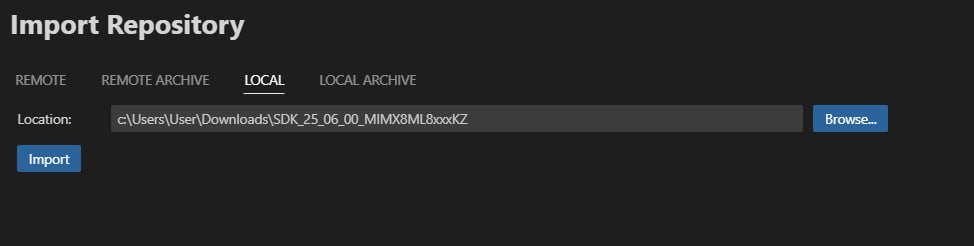
\includegraphics[width=0.75\linewidth]{import repository.png}
    \caption{Import Repo}
    \label{fig:placeholder}
\end{figure}

% TODO: Screenshot of MCUXpresso extension panel showing imported repository

\textbf{Step 3: Configure Debug Probe}

During this internship, \textbf{Segger J-Link} was used for JTAG debugging.

\begin{enumerate}
    \item At the bottom below projects, you are able to see the different debug probes available
    \item Debug Probe: Select "SEGGER J-Link"
    \item Vscode should prompt you about mcuxpresso installer. Use it to download all the necessary tools needed such as MCUXpresso sdk developer and the j link debug probes software pack
    \item Verify connection: "Debug Adapter" → "Test Connection"
\end{enumerate}

\begin{figure}[H]
    \centering
    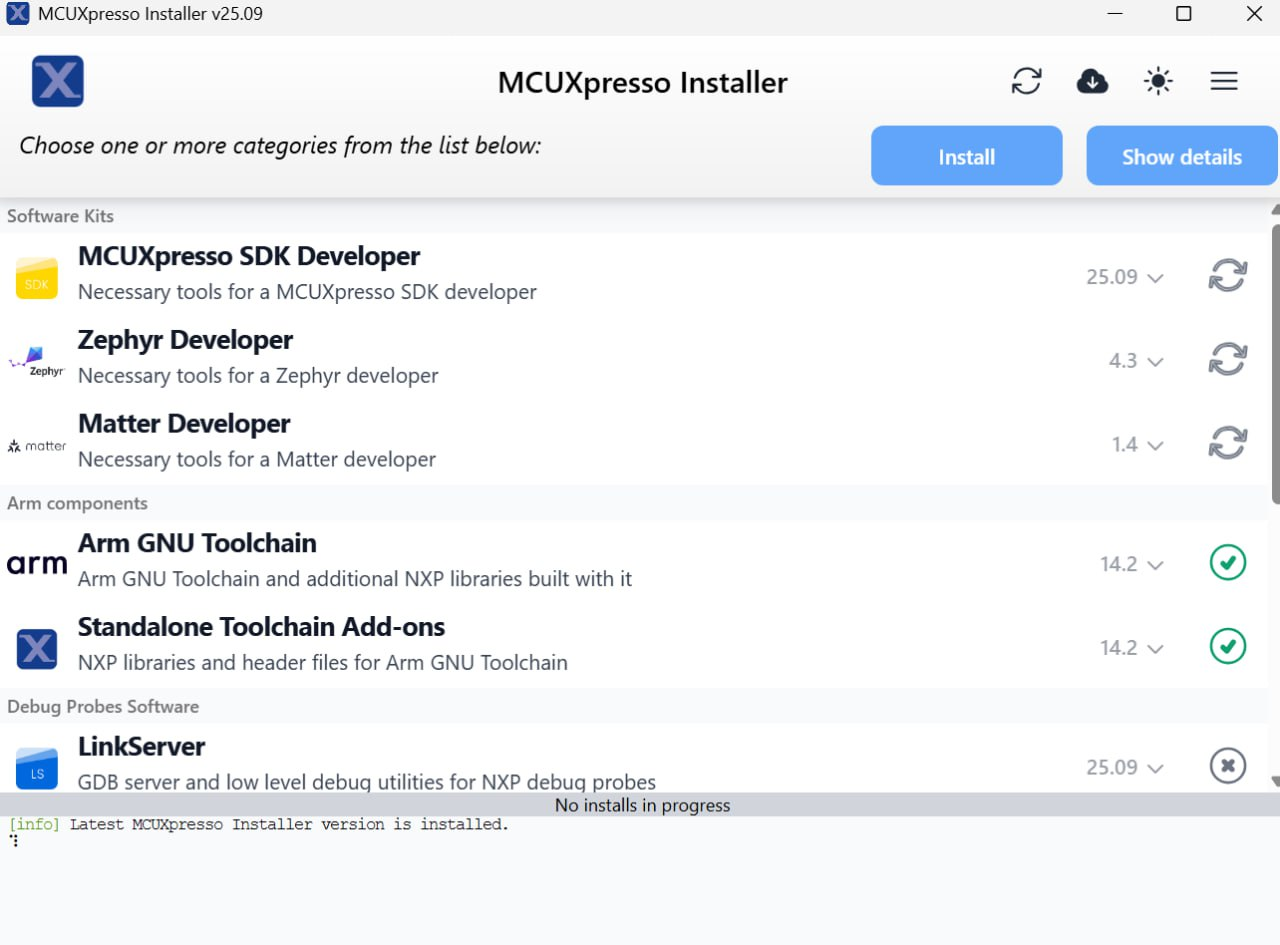
\includegraphics[width=0.75\linewidth]{mcuxpresso installer.png}
    \caption{mcuxpresso installer}
    \label{fig:placeholder}
\end{figure}


\textbf{Supported debug probes:}
\begin{itemize}
    \item Segger J-Link (used during internship) 
    \item NXP LPC-Link2
    \item PEMicro OpenSDA
    \item CMSIS-DAP
\end{itemize}

% TODO: Photo of J-Link connected to EVK board JTAG header

\subsection{Starting a New Project from Example}

\textbf{Example: Starting a PWM project}

\begin{enumerate}
    \item MCUXpresso extension → "Import Example Project"
    \item Repository: Select your imported SDK
    \item Board: evkmimx8mp
    \item Navigate: \texttt{driver\_examples > pwm > pwm}
    \item Click "Import"
    \item Project appears in workspace
\end{enumerate}


\begin{figure}[H]
    \centering
    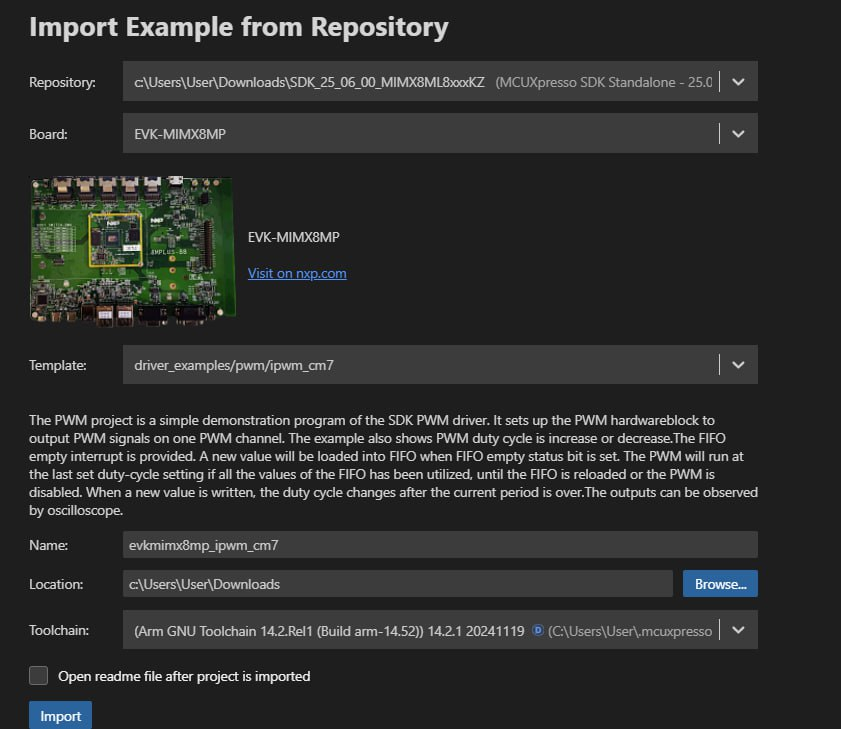
\includegraphics[width=0.5\linewidth]{example project .png}
    \caption{PWM example}
    \label{fig:placeholder}
\end{figure}

% TODO: Screenshot of Import Example dialog

The imported project contains:
\begin{verbatim}
pwm_example/
|-- source/
|   |-- main.c           # Main application code
|   |-- pin_mux.c        # Pin configuration (IOMUXC)
|   |-- pin_mux.h
|   |-- board.c          # Board initialization
|   |-- board.h
|   +-- clock_config.c   # Clock tree configuration
|
|-- armgcc/
|   |-- CMakeLists.txt   # Build configuration
|   +-- MIMX8ML8xxxxx_cm7_ram.ld  # Linker script ⭐
|
+-- .vscode/
    |-- launch.json      # Debug configuration
    +-- tasks.json       # Build tasks
\end{verbatim}

\begin{important}
\textbf{Finding the Linker Script:}

The linker script is located at:
\begin{center}
\texttt{armgcc/MIMX8ML8xxxxx\_cm7\_ram.ld}
\end{center}

You can view and edit it directly in VS Code. This file defines:
\begin{itemize}
    \item Memory regions (ITCM, DTCM, DDR)
    \item Section placement (.text, .data, .bss)
    \item Stack and heap sizes
\end{itemize}

See Section \ref{sec:linker_script} for detailed linker script configuration and testing.
\end{important}

\subsection{Key Files to Modify}

When working with examples, these are the main files you'll edit:

\textbf{1. main.c/pwm.c (examplename.c) - Application Logic}

Contains:
\begin{itemize}
    \item \texttt{main()} function
    \item Peripheral initialization
    \item Application loop
    \item Interrupt handlers
\end{itemize}

\textbf{2. pin\_mux.c - Pin Configuration}

Contains:
\begin{itemize}
    \item \texttt{BOARD\_InitPins()} - IOMUXC configuration
    \item Pin mux settings (ALT functions)
    \item Pad electrical properties (pull-ups, drive strength)
\end{itemize}

Example from I2C:
\begin{lstlisting}[language=c]
void BOARD_InitPins(void) {
    IOMUXC_SetPinMux(IOMUXC_I2C3_SCL_I2C3_SCL, 1U);
    IOMUXC_SetPinConfig(IOMUXC_I2C3_SCL_I2C3_SCL, 
        IOMUXC_SW_PAD_CTL_PAD_ODE_MASK | /* ... */);
}
\end{lstlisting}

\textbf{3. board.c - Board Initialization}

Contains:
\begin{itemize}
    \item \texttt{BOARD\_InitHardware()} - Calls all init functions
    \item \texttt{BOARD\_InitDebugConsole()} - UART console setup
    \item Clock initialization
    \item System configuration
\end{itemize}

\textbf{4. MIMX8ML8xxxxx\_cm7\_ram.ld - Linker Script}

Located in \texttt{armgcc/} folder. Contains:
\begin{itemize}
    \item Memory region definitions (ITCM, DTCM, DDR)
    \item Section placement (.text, .data, .bss, .ncache)
    \item Stack and heap sizes
\end{itemize}

\subsection{Building and Debugging}

\textbf{Build Process:}

\begin{enumerate}
    \item Open project in VS Code
    \item Terminal → Run Build Task (Ctrl+Shift+B)
    \item Or: MCUXpresso extension → "Build"
    \item Output: \texttt{armgcc/release/pwm\_example.elf}
\end{enumerate}

Check build output for memory usage:
\begin{lstlisting}
Memory region         Used Size  Region Size  %age Used
m_interrupts:           680 B         1 KB    66.41%
m_text:               18536 B       127 KB    14.25%
m_data:                2184 B       128 KB     1.67%
m_data2:                  0 B        16 MB     0.00%
\end{lstlisting}

% TODO: Screenshot of successful build output in terminal

\textbf{Debug Process:}

\begin{enumerate}
    \item Connect J-Link to EVK board JTAG header
    \item Power on EVK board
    \item VS Code → Run and Debug (Ctrl+Shift+D)
    \item Select "Debug (J-Link)"
    \item Press F5 or click "Start Debugging"
\end{enumerate}

\textbf{What happens when you press Debug/F5:}
\begin{enumerate}
    \item J-Link connects to M7 core via JTAG
    \item Firmware is loaded directly to TCM/DDR
    \item M7 is reset and halted at \texttt{main()}
    \item Debugger attaches
    \item You can now:
    \begin{itemize}
        \item Set breakpoints (click left of line number)
        \item Step through code (F10=step over, F11=step into)
        \item Inspect variables (hover or watch window)
        \item View registers
        \item Monitor UART output (using mobaxterm)
        \item Modify variables in real-time
    \end{itemize}
\end{enumerate}

% TODO: Screenshot of VS Code debug session with breakpoint hit

\textbf{Common debugging workflow:}
\begin{lstlisting}[language=c]
int main(void) {
    BOARD_InitHardware();  // <- Set breakpoint here (click line number)
    PRINTF("Starting...\r\n");
    
    // Initialize peripheral
    I2C_MasterInit(DEMO_I2C, &config, srcClkHz);
    
    // Your code
    while (1) {
        // Step through with F10 to debug logic
        read_sensor();
        process_data();
    }
}
\end{lstlisting}

\textbf{Advantages over remoteproc method:}
\begin{itemize}
    \item \textbf{Instant reload:} Press F5, code reloads in 2 seconds
    \item \textbf{No file copying:} No need to SCP ELF to board
    \item \textbf{Real debugging:} Breakpoints, step-through, variable inspection
    \item \textbf{Fast iteration:} Edit → Build → Debug cycle is <10 seconds
\end{itemize}

\subsection{Working with GitHub Examples}

All examples from this internship are available on GitHub:

\begin{gitref}
\textbf{GitHub Repository:}

\url{https://github.com/yulyuri/firmware-and-dts}

Contains:
\begin{itemize}
    \item Complete working examples (I2C, UART, PWM, CAN, DMA)
    \item Device tree files
    \item Linker scripts
    \item Pin mux configurations
\end{itemize}

\textbf{To use an example:}
\begin{enumerate}
    \item Try to download the example code it was based from
    \item Build project (Ctrl+Shift+B)
    \item Examine the key files and simply copy and paste over them !:
    \begin{itemize}
        \item \texttt{source/main.c} - Application logic
        \item \texttt{source/pin\_mux.c} - Pin configuration
        \item \texttt{source/board.c} - Hardware initialization
        \item \texttt{armgcc/MIMX8ML8xxxxx\_cm7\_ram.ld} - Linker script (only relevant to the linker script example)
    \end{itemize}
    \item Debug with J-Link (F5)
\end{enumerate}
\end{gitref}

\subsection{My Typical Development Cycle}

\begin{enumerate}
    \item \textbf{Start from example:} Import closest matching example from SDK
    \item \textbf{Modify pins:} Edit \texttt{pin\_mux.c} for your hardware
    \item \textbf{Implement logic:} Edit \texttt{main.c} for your application
    \item \textbf{Build:} Ctrl+Shift+B (watch for memory usage)
    \item \textbf{Debug:} F5 with J-Link connected
    \item \textbf{Test:} Verify functionality with  PRINTF functions
    \item \textbf{Iterate:} Fix bugs, optimize, repeat steps 4-6
    \item \textbf{Deploy:} When stable, deploy via remoteproc (Section \ref{sec:remoteproc})
\end{enumerate}

\textbf{Pro tips:}
\begin{itemize}
    \item Always start from working SDK example
    \item Make incremental changes and test frequently
    \item Use PRINTF liberally for debugging
    \item Check memory usage after every build
    \item Keep backup of working versions
    \item Document pin assignments and configurations
    \item Use Git for version control
\end{itemize}

\subsection{Printf and Floating Point}

By default, printf doesn't support floating point to save code size.

\textbf{To enable float printf:}

Add to \texttt{CMakeLists.txt}:
\begin{lstlisting}[language=cmake]
target_compile_definitions(${MCUX_SDK_PROJECT_NAME} 
    PRIVATE PRINTF_FLOAT_ENABLE=1)
\end{lstlisting}

Include stdio explicitly in \texttt{main.c}:
\begin{lstlisting}[language=c]
#include <stdio.h>

// Now works:
float temp = 25.6;
printf("Temperature: %.2f C\n", temp);
\end{lstlisting}

\begin{docref}
\textbf{Printf Float Support:}

\url{https://community.nxp.com/t5/MCUXpresso-IDE/To-complement-solution-how-to-printf-float-number-in-MCUXpresso/td-p/1431699}

Detailed guide on enabling float formatting in fsl\_debug\_console.
\end{docref}

\section{Memory Architecture}

\subsection{Complete Memory Map}

Understanding the memory map is critical for M7 development:

\begin{center}
\begin{tabular}{|l|l|p{6cm}|}
\hline
\textbf{Address Range} & \textbf{Size} & \textbf{Purpose} \\
\hline
\multicolumn{3}{|c|}{\textbf{M7 Fast Memory (TCM)}} \\
\hline
0x00000000 - 0x0001FFFF & 128 KB & ITCM (code execution) \\
\hline
0x20000000 - 0x2001FFFF & 128 KB & DTCM (data, stack, heap) \\
\hline
\multicolumn{3}{|c|}{\textbf{Shared On-Chip RAM}} \\
\hline
0x00900000 - 0x0096FFFF & 448 KB & OCRAM (shared with A53) \\
\hline
\multicolumn{3}{|c|}{\textbf{DDR Memory Regions}} \\
\hline
0x40000000 - 0x54FFFFFF & ~336 MB & Linux reserved (A53 only) \\
\hline
0x55000000 - 0x550FFFFF & ~1 MB & RPMsg communication \\
\hline
0x80000000 - 0x80FFFFFF & 16 MB & M7 firmware \& data (NonCacheable) \\
\hline
0x90000000+ & ~3.5 GB & Linux system memory \\
\hline
\multicolumn{3}{|c|}{\textbf{Peripherals}} \\
\hline
0x30000000 - 0x3FFFFFFF & --- & Hardware registers (UART, I2C, etc.) \\
\hline
\end{tabular}
\end{center}

% TODO: Add full memory map diagram showing all regions

\subsection{TCM: Tightly Coupled Memory}

\textbf{What is TCM?}

TCM (Tightly Coupled Memory) is ultra-fast, deterministic memory directly connected to the M7 core:
\begin{itemize}
    \item \textbf{Zero wait states:} Single-cycle access (no cache misses)
    \item \textbf{Deterministic timing:} Critical for real-time control loops
    \item \textbf{Power efficient:} Stays powered in suspend mode
    \item \textbf{DDR-independent:} M7 runs even when DDR is in self-refresh
\end{itemize}

\textbf{TCM is split into two regions:}

\begin{center}
\begin{tabular}{|l|l|l|l|}
\hline
\textbf{Region} & \textbf{Address} & \textbf{Size} & \textbf{Contents} \\
\hline
ITCM & 0x00000000 & 128 KB & Code (.text, .rodata) \\
\hline
DTCM & 0x20000000 & 128 KB & Data (.data, .bss, stack, heap) \\
\hline
\end{tabular}
\end{center}

\begin{important}
\textbf{Why TCM is Critical for Suspend Mode:}

If M7 firmware runs from DDR and the system enters suspend:
\begin{itemize}
    \item DDR enters self-refresh mode (powered down)
    \item M7 cannot fetch instructions → crash
    \item M7 cannot access data → undefined behavior
\end{itemize}

\textbf{Solution:} Flight control firmware MUST run from TCM to support low-power operation while A53 is suspended.
\end{important}

\subsection{DDR Memory for M7}

Only 16 MB of DDR is reserved for M7 use (configured in device tree):

\textbf{DDR allocation:}
\begin{itemize}
    \item Total DDR: 4 GB
    \item Linux (A53): ~3.9 GB
    \item M7 reserved: 16 MB at 0x80000000
    \item RPMsg buffers: ~4 MB at 0x55000000
\end{itemize}

\textbf{When to use DDR:}
\begin{itemize}
    \item Large buffers (> 128 KB) that don't fit in TCM
    \item DMA buffers (must be NonCacheable)
    \item Shared data with A53 cores
    \item Sensor data logs
    \item Camera frame buffers
\end{itemize}

\textbf{Important: DDR is NOT used automatically}
\begin{itemize}
    \item Normal variables do NOT overflow to DDR
    \item Only explicit NonCacheable sections go to DDR
    \item If DTCM fills up (>128 KB), build fails
\end{itemize}

\subsection{Cacheable vs NonCacheable Memory}

\textbf{What is Cache?}

Cache is super-fast memory between CPU and slower DDR:

\begin{verbatim}
CPU → Cache Hit (fast, 0-1 cycle)
CPU → Cache Miss → DDR (slow, 100+ cycles)
\end{verbatim}

\textbf{Cacheable Data (Default):}
\begin{lstlisting}[language=c]
int sensor_value = 123;  // Cacheable by default
\end{lstlisting}

\begin{itemize}
    \item CPU reads from DDR → copies to cache
    \item Next read is super fast from cache
    \item Good for: Normal variables only M7 uses
\end{itemize}

\textbf{NonCacheable Data (Special Cases):}
\begin{lstlisting}[language=c]
__attribute__((section("NonCacheable")))
uint8_t shared_buffer[1024];  // NonCacheable
\end{lstlisting}

\begin{itemize}
    \item CPU reads directly from DDR (no cache)
    \item Slower (100+ cycles per access)
    \item Good for: Shared data or DMA buffers
\end{itemize}

\textbf{When to use NonCacheable:}
\begin{enumerate}
    \item \textbf{RPMsg buffers:} Shared between M7 and A53
    \begin{itemize}
        \item Both cores see changes immediately
        \item No cache coherency issues
    \end{itemize}
    
    \item \textbf{DMA buffers:} Hardware writes directly
    \begin{itemize}
        \item DMA writes to DDR
        \item M7 sees DMA updates immediately
    \end{itemize}
    
    \item \textbf{Large buffers:} Too big for DTCM
    \begin{itemize}
        \item Camera frames
        \item Large sensor logs
        \item Audio/video buffers
    \end{itemize}
\end{enumerate}

\begin{important}
\textbf{Cache Coherency Problems:}

\textbf{Without NonCacheable attribute:}
\begin{itemize}
    \item CPU writes data → stays in cache → DMA reads old RAM value 
    \item DMA writes data → in RAM only → CPU reads old cached value 
\end{itemize}

\textbf{Solution:} Always use NonCacheable for DMA and shared buffers!
\end{important}
\subsection{Linker Script Configuration}
\label{sec:linker_script}

The linker script (\texttt{MIMX8ML8xxxxx\_cm7\_ram.ld}) defines memory regions and section placement.
Please take note that the default linker script differs from example to example

\textbf{Location:} \texttt{armgcc/MIMX8ML8xxxxx\_cm7\_ram.ld}

\textbf{Memory region definitions:}

\begin{lstlisting}[language=c]
MEMORY
{
  m_interrupts (RX) : ORIGIN = 0x00000000, LENGTH = 0x00000400  // 1 KB
  m_text       (RX) : ORIGIN = 0x00000400, LENGTH = 0x0001FC00  // 127 KB
  m_data       (RW) : ORIGIN = 0x20000000, LENGTH = 0x00020000  // 128 KB
  m_data2      (RW) : ORIGIN = 0x80000000, LENGTH = 0x01000000  // 16 MB
}
\end{lstlisting}

\begin{center}
\begin{tabular}{|l|l|l|p{5cm}|}
\hline
\textbf{Region} & \textbf{Address} & \textbf{Size} & \textbf{Purpose} \\
\hline
m\_interrupts & 0x00000000 & 1 KB & Interrupt Vector Table (ITCM) \\
\hline
m\_text & 0x00000400 & 127 KB & Program Code \& Constants (ITCM) \\
\hline
m\_data & 0x20000000 & 128 KB & Variables, Stack, Heap (DTCM) \\
\hline
m\_data2 & 0x80000000 & 16 MB & NonCacheable / DMA Data (DDR) \\
\hline
\end{tabular}
\end{center}

\textbf{Standard section placement:}

\begin{lstlisting}[language=c]
SECTIONS
{
  /* Code → ITCM */
  .text :
  {
    KEEP(*(.isr_vector))  /* Interrupt vectors */
    *(.text*)              /* All functions */
    *(.rodata*)            /* Constants */
  } > m_text

  /* Initialized variables → DTCM */
  .data :
  {
    *(.data*)      /* e.g., int x = 42; */
  } > m_data

  /* Uninitialized variables → DTCM */
  .bss :
  {
    *(.bss*)       /* e.g., int y; */
  } > m_data

  /* NonCacheable/DMA → DDR */
  .ncache :
  {
    *(NonCacheable)
  } > m_data2

  /* Stack → DTCM */
  .stack :
  {
    . = ALIGN(8);
    . += STACK_SIZE;
  } > m_data

  /* Heap → DTCM */
  .heap :
  {
    . = ALIGN(8);
    . += HEAP_SIZE;
  } > m_data
}
\end{lstlisting}

\textbf{Custom sections for DDR code/data (Added during testing):}

To enable selective placement of code in DDR, these sections were added:

\begin{lstlisting}[language=c]
SECTIONS
{
  /* ... standard sections above ... */
  
  /* Code placed in DDR (for large, non-critical functions) */
  .text_ddr :
  {
    . = ALIGN(4);
    *(.text_ddr)
    *(.text_ddr*)
    . = ALIGN(4);
  } > m_data2

  /* Read-only data in DDR (for large lookup tables, constants) */
  .rodata_ddr :
  {
    . = ALIGN(4);
    *(.rodata_ddr)
    *(.rodata_ddr*)
    . = ALIGN(4);
  } > m_data2
  
  /* ... rest of sections ... */
}
\end{lstlisting}

\textbf{Stack and Heap Configuration:}

Default sizes:
\begin{lstlisting}[language=c]
HEAP_SIZE  = 0x0400;  // 1 KB
STACK_SIZE = 0x0400;  // 1 KB
\end{lstlisting}

Recommended for flight control:
\begin{lstlisting}[language=c]
HEAP_SIZE  = 0x2000;  // 8 KB
STACK_SIZE = 0x2000;  // 8 KB
\end{lstlisting}

\textbf{Checking Memory Usage After Build:}

After compilation, terminal shows:
\begin{lstlisting}
Memory region         Used Size  Region Size  %age Used
m_interrupts:           680 B         1 KB    66.41%
m_text:               18536 B       127 KB    14.25%  <- Code in TCM
m_data:                2184 B       128 KB     1.67%  <- Variables in TCM
m_data2:               2048 B        16 MB     0.01%  <- DDR (if .text_ddr used)
\end{lstlisting}

\begin{important}
\textbf{Memory Overflow:}

If you exceed DTCM (128 KB):
\begin{itemize}
    \item Build will fail with "region overflow" error
    \item Move large buffers to DDR using custom sections
    \item Or reduce buffer sizes
    \item Cannot automatically overflow to DDR
\end{itemize}
\end{important}

\subsection{Linker Script Testing: TCM vs DDR Performance}

During development, comprehensive testing was conducted to quantify the performance difference between TCM and DDR execution.

\begin{gitref}
\textbf{Complete Test Code:}

\url{https://github.com/yulyuri/firmware-and-dts/tree/master/M7/linker_script}

Contains full source code for all three benchmark tests with detailed comments.
\end{gitref}

\subsubsection{Test Setup and Macros}

To enable easy comparison, the following macros were defined:

\begin{lstlisting}[language=c]
/* Placement control macros */
#define FAST_CODE   /* Nothing - default is TCM */
#define SLOW_CODE   __attribute__((section(".text_ddr")))
#define SLOW_DATA   __attribute__((section(".rodata_ddr")))
\end{lstlisting}

\textbf{How these macros work:}
\begin{itemize}
    \item \texttt{FAST\_CODE}: Empty macro, functions default to .text section → ITCM
    \item \texttt{SLOW\_CODE}: Tells linker to place function in .text\_ddr section → DDR
    \item \texttt{SLOW\_DATA}: Tells linker to place data in .rodata\_ddr section → DDR
\end{itemize}

\textbf{Timing measurement:}

\begin{lstlisting}[language=c]
// Enable DWT cycle counter
static inline void start_timer(void) {
    CoreDebug->DEMCR |= CoreDebug_DEMCR_TRCENA_Msk;
    DWT->CTRL |= DWT_CTRL_CYCCNTENA_Msk;
    DWT->CYCCNT = 0;
}

// Read cycle count
static inline uint32_t get_cycles(void) {
    return DWT->CYCCNT;  // Returns CPU cycles elapsed
}
\end{lstlisting}

At 800 MHz, each cycle = 1.25 ns. This provides precise microsecond-level timing.

\subsubsection{Test 1: Simple Loop (Integer Arithmetic)}

\textbf{Test code:}

\begin{lstlisting}[language=c]
FAST_CODE
uint32_t simple_loop_fast(uint32_t count) {
    uint32_t sum = 0;
    for (uint32_t i = 0; i < count; i++) {
        sum += i;
    }
    return sum;
}

SLOW_CODE
uint32_t simple_loop_slow(uint32_t count) {
    uint32_t sum = 0;
    for (uint32_t i = 0; i < count; i++) {
        sum += i;
    }
    return sum;
}

// Test with 5000 iterations
\end{lstlisting}

\textbf{Results:}
\begin{center}
Code in TCM  was 22x faster
\end{center}

\subsubsection{Test 2: FFT Computation (Floating Point)}

\textbf{Test code:}

256-point Fast Fourier Transform with bit-reversal and butterfly operations:

\begin{lstlisting}[language=c]
FAST_CODE
void compute_fft_fast(complex_t *data, uint32_t n) {
    // Bit reversal reordering
    // Butterfly computation with twiddle factors
    // Multiple stages with sine/cosine calculations
}

SLOW_CODE
void compute_fft_slow(complex_t *data, uint32_t n) {
    // Identical algorithm, different memory location
}
\end{lstlisting}

\textbf{Results:}
\begin{center}
Code in TCM  was 7.8x faster
\end{center}

\subsubsection{Test 3: Array Access (Sequential Read)}

\textbf{Test code:}

\begin{lstlisting}[language=c]
float array_fast[500];  // Default → DTCM

SLOW_DATA const float array_slow[500] = {[0 ... 499] = 1.0f};  // DDR

// Read all elements sequentially
volatile float sum = 0;
for (int i = 0; i < 500; i++) {
    sum += array[i];
}
\end{lstlisting}

\textbf{Results:}
\begin{center}
Code in TCM  was 7x faster
\end{center}

\subsubsection{Performance Analysis}

\textbf{The possible reasons why I think TCM is faster:}

\begin{enumerate}
    \item \textbf{Zero wait states:}
    \begin{itemize}
        \item TCM: Single-cycle access (1 cycle = 1.25 ns)
        \item DDR: 100-200+ cycles per cache miss
    \end{itemize}
    
    \item \textbf{No cache misses:}
    \begin{itemize}
        \item TCM: Always hit (deterministic)
        \item DDR: Cache misses cause stalls
    \end{itemize}
    
    \item \textbf{Instruction fetch:}
    \begin{itemize}
        \item TCM: Fetch and execute simultaneously
        \item DDR: Pipeline stalls on cache misses
    \end{itemize}
    
    \item \textbf{DDR refresh cycles:}
    \begin{itemize}
        \item DDR must periodically refresh (unavailable during refresh)
        \item TCM: Always available
    \end{itemize}
\end{enumerate}

\textbf{Test-specific observations (might be wrong, please verify):}

\begin{itemize}
    \item \textbf{Test 1 (22x speedup):} Small loop fits entirely in instruction cache initially, but frequent jumps cause cache thrashing in DDR version. TCM has no such penalty.
    
    \item \textbf{Test 2 (7.8x speedup):} FFT has complex control flow (nested loops, bit reversal). Many instruction cache misses in DDR. Large code size exceeds cache capacity.
    
    \item \textbf{Test 3 (7x speedup):} Sequential array access benefits from DDR burst mode and prefetching, which partially mitigates latency. Still slower than TCM's zero-wait access.
\end{itemize}

\begin{important}
\textbf{Remaining Investigation Needed:}

Several aspects were not fully explored during this internship:

\begin{enumerate}
    \item \textbf{Cache behavior under different workloads:}
    \begin{itemize}
        \item Why does Test 1 show 22x difference but Test 2 only 7.8x?
        \item How does cache size (32 KB I-cache, 32 KB D-cache) affect each test?
        \item What is the exact cache miss rate for each test?
    \end{itemize}

    
    
    \item \textbf{Mixed TCM/DDR strategies, when exactly we use what?:}
    \begin{itemize}
        \item Critical loops in TCM, everything else in DDR?
        \item Can interrupt handlers in TCM call DDR functions safely?
        \item What is the overhead of TCM↔DDR function calls?
    \end{itemize}
    
    
\end{enumerate}

\end{important}

\textbf{Possible design for flight control in the future based on results:}

Based on these results:
\begin{itemize}
    \item \textbf{Always in TCM:}
    \begin{itemize}
        \item Interrupt handlers
        \item Control loops (PID, motor mixing)
        \item Sensor reading functions
        \item Safety-critical code
    \end{itemize}
    
    \item \textbf{Can be in DDR:}
    \begin{itemize}
        \item Telemetry formatting
        \item Logging functions
        \item Configuration parsing
        \item Non-real-time diagnostics
    \end{itemize}
    
    \item \textbf{Measured decision needed:}
    \begin{itemize}
        \item State estimation (Kalman filters) - depends on complexity
        \item Path planning - depends on update rate required
        \item Sensor fusion - measure actual performance
    \end{itemize}
\end{itemize}

\textbf{Summary:} TCM provides 7-22x performance improvement depending on workload characteristics. For deterministic real-time performance, keep critical code in TCM. The exact reasons for variation between tests require further investigation with cache profiling tools.

\section{Device Tree and Boot Methods}
\label{sec:remoteproc}

\subsection{Device Tree Configuration}

The M7 core must be defined in the Linux device tree for proper resource allocation. You can refer to the default imx8mp rpmsg dts:

\begin{lstlisting}[language=c]
imx8mp-cm7 {
    compatible = "fsl,imx8mn-cm7";  // Used for both 8MN and 8MP
    rsc-da = <0x55000000>;           // Resource table address
    clocks = <&clk IMX8MP_CLK_M7_DIV>;
    mbox-names = "tx", "rx", "rxdb";
    mboxes = <&mu 0 1>, <&mu 1 1>, <&mu 3 1>;  // MU channels
    memory-region = <&vdev0vring0>, <&vdev0vring1>, <&vdevbuffer>,
                    <&m4_reserved>, <&m7_ddr_alias>, 
                    <&m7_itcm>, <&m7_dtcm>;
    status = "okay";
};
\end{lstlisting}

\subsection{Reserved Memory Regions}

Critical memory regions must be reserved for M7 use:

\begin{lstlisting}[language=c]
reserved-memory {
    // Main DDR region for M7 firmware and data
    m4_reserved: m4@0x80000000 {
        no-map;
        reg = <0 0x80000000 0 0x1000000>;  // 16 MB in DDR
    };

    // Instruction Tightly Coupled Memory
    m7_itcm: m4@0x7E0000 {
        no-map;
        reg = <0 0x7E0000 0 0x20000>;  // 128 KB ITCM
    };

    // Data Tightly Coupled Memory
    m7_dtcm: m4@0x800000 {
        no-map;
        reg = <0 0x800000 0 0x20000>;  // 128 KB DTCM
    };

    // RPMsg communication buffers
    vdev0vring0: vdev0vring0@55000000 {
        reg = <0 0x55000000 0 0x8000>;  // 32 KB TX ring
    };

    vdev0vring1: vdev0vring1@55008000 {
        reg = <0 0x55008000 0 0x8000>;  // 32 KB RX ring
    };

    vdevbuffer: vdevbuffer@55400000 {
        reg = <0 0x55400000 0 0x100000>;  // 1 MB shared buffer
    };
};
\end{lstlisting}

\begin{gitref}
\textbf{Device Tree Files:}

Complete default device tree with M7 configuration:

\url{https://github.com/yulyuri/firmware-and-dts/blob/master/SCP%20files/imx8mp-evk-rpmsg.dts}
\end{gitref}

\subsection{Understanding Remoteproc and RPMsg}

\textbf{Remoteproc (Remote Processor):}
\begin{itemize}
    \item Linux kernel framework for managing remote processors
    \item Handles M7 firmware loading from \texttt{/lib/firmware/}
    \item Controls M7 power state (start, stop, restart)
    \item Manages resource table and memory allocation
    \item Exposed via sysfs: \texttt{/sys/class/remoteproc/}
\end{itemize}

\textbf{RPMsg (Remote Processor Messaging):}
\begin{itemize}
    \item Communication protocol between A53 (Linux) and M7 (RTOS)
    \item Built on top of VirtIO shared memory buffers
    \item Provides virtual TTY devices: \texttt{/dev/ttyRPMSG*}
    \item Bidirectional message passing
    \item Examples: string echo, command/response, sensor data streaming
\end{itemize}

\subsection{M7 Boot Sequence}

The M7 can be started at different points in the boot process:

\textbf{Option 1: Boot from U-Boot (Early Start)}

\begin{lstlisting}[language=bash]
# In U-Boot console, before booting Linux:
u-boot=> run prepare_mcore
u-boot=> boot
\end{lstlisting}

\textbf{What \texttt{prepare\_mcore} does:}
\begin{itemize}
    \item Loads M7 firmware from SD card or eMMC
    \item Sets shared memory flag indicating M7 is pre-started
    \item Enables M7 clock
    \item Starts M7 execution
    \item Linux remoteproc detects M7 is already running
\end{itemize}

\textbf{Option 2: Boot from Linux (Runtime Start)}

\textbf{This is the method you use when NOT debugging with J-Link.}

\begin{lstlisting}[language=bash]
# Check available remoteproc instances
ls /sys/class/remoteproc/
# Typically: remoteproc0 (M7), remoteproc1 (DSP)

# Load firmware and start M7
echo your_firmware.elf > /sys/class/remoteproc/remoteproc0/firmware
echo start > /sys/class/remoteproc/remoteproc0/state

# Check status
cat /sys/class/remoteproc/remoteproc0/state
# Should show: running
\end{lstlisting}

\begin{important}
\textbf{Clock Dependency Issue:}

From NXP AN5317: "For i.MX 8M platforms, the root clock for M7 must be kept always enabled by Linux to load firmware and start Cortex-M7."

\textbf{If starting M7 from Linux remoteproc:}
\begin{itemize}
    \item Linux clock driver may gate M7 clock by default
    \item You must modify kernel driver: \texttt{drivers/clk/imx/clk-composite-8m.c}
    \item Skip gate registration for M7's root clock
    \item Otherwise, M7 will fail to start or crash unexpectedly
\end{itemize}

\textbf{If starting M7 from U-Boot:}
\begin{itemize}
    \item Clock is enabled during \texttt{prepare\_mcore}
    \item Linux inherits the clock state
    \item No kernel driver modification needed
    \item \textbf{Recommended approach for flight control applications}
\end{itemize}
\end{important}

\subsection{Initial Testing with NXP SDK Examples}

NXP provides pre-built example firmware:

\begin{lstlisting}[language=bash]
# Check available firmware
ls /lib/firmware/
# Look for: imx8mp_m7_TCM_rpmsg_lite_str_echo_rtos.elf

# Boot from U-Boot:
u-boot=> run prepare_mcore
u-boot=> boot

# After Linux boots, load RPMsg TTY driver
modprobe imx_rpmsg_tty

# Check for RPMsg devices
ls /dev/ttyRPMSG*
# Should see: /dev/ttyRPMSG0

# Test string echo
echo "hello" > /dev/ttyRPMSG0
cat /dev/ttyRPMSG0
# Should echo back: hello
\end{lstlisting}

\textbf{Verify M7 status:}
\begin{lstlisting}[language=bash]
# Check remoteproc state
cat /sys/class/remoteproc/remoteproc0/state
# If U-Boot started M7: shows "detached" or "running"
# If not started: shows "offline"

# Check kernel messages
dmesg | grep rpmsg
# Should see messages about RPMsg channel creation
\end{lstlisting}

\subsection{Deploying Your Firmware }

After developing with J-Link, deploy to production:

\begin{lstlisting}[language=bash]
# Copy ELF from development machine to board
scp elf_file_path root@192.168.1.100:/lib/firmware/

# On target board (via SSH or serial console)
echo my_flight_control.elf > /sys/class/remoteproc/remoteproc0/firmware
echo start > /sys/class/remoteproc/remoteproc0/state

# Verify running
cat /sys/class/remoteproc/remoteproc0/state
# Should show: running

# Check M7 console output (if using RPMsg TTY)
cat /dev/ttyRPMSG0

# Stop M7 (if needed)
echo stop > /sys/class/remoteproc/remoteproc0/state
\end{lstlisting}

\textbf{Comparison: Development vs Production}

\begin{center}
\begin{tabular}{|l|l|l|}
\hline
\textbf{Aspect} & \textbf{J-Link (Dev)} & \textbf{Remoteproc (Prod)} \\
\hline
Speed & Fast (2 sec reload) & Slow (copy + reload) \\
\hline
Debugging & Full breakpoints & None (use PRINTF) \\
\hline
Iteration & Instant & Manual file copy \\
\hline
Use case & Development & Production/Field \\
\hline
Hardware & J-Link required & No extra hardware \\
\hline
\end{tabular}
\end{center}
\section{Peripheral Development}

This section covers practical peripheral usage with actual code examples tested during the internship. All working examples are available on GitHub.

\begin{important}
\textbf{Security Note - External Device Whitelisting:}

Before connecting ANY external devices (oscilloscopes, logic analyzers, USB drives, SD cards) to your development machine:
\begin{itemize}
    \item Register device with IT Concierge FIRST
    \item Get device whitelisted before connecting
    \item Failure to do so triggers security alerts
    \item Personal SD cards with work files will be flagged by cybersecurity
\end{itemize}

Lesson learned: My SD card containing Linux images for the M7 was connected without whitelisting and triggered a security incident. Please don't make this stupid mistake!
\end{important}

\subsection{Pin Muxing (IOMUXC)}

Before using any peripheral, pins must be muxed to the correct function.

\textbf{Pin mux example for I2C3:}

\begin{lstlisting}[language=c]
void BOARD_InitPins(void)
{
    // Route pads to I2C3 function (ALT4)
    IOMUXC_SetPinMux(IOMUXC_I2C3_SCL_I2C3_SCL, 1U);  // SION=1
    IOMUXC_SetPinMux(IOMUXC_I2C3_SDA_I2C3_SDA, 1U);

    // Configure electrical properties for I2C
    const uint32_t i2c_pad =
        IOMUXC_SW_PAD_CTL_PAD_ODE_MASK   |  // Open-drain (required)
        IOMUXC_SW_PAD_CTL_PAD_FSEL_MASK  |  // Fast slew
        IOMUXC_SW_PAD_CTL_PAD_PE_MASK    |  // Pull enable
        IOMUXC_SW_PAD_CTL_PAD_PUE_MASK   |  // Pull-up (not down)
        IOMUXC_SW_PAD_CTL_PAD_PUS(2U)    |  // Weak pull-up
        IOMUXC_SW_PAD_CTL_PAD_DSE(2U)    |  // Medium drive
        IOMUXC_SW_PAD_CTL_PAD_HYS_MASK;     // Schmitt trigger

    IOMUXC_SetPinConfig(IOMUXC_I2C3_SCL_I2C3_SCL, i2c_pad);
    IOMUXC_SetPinConfig(IOMUXC_I2C3_SDA_I2C3_SDA, i2c_pad);
}
\end{lstlisting}

% TODO: Add i.MX8MP pinout diagram
% TODO: Add pin mux register screenshots

\textbf{Understanding pad control bits:}
\begin{itemize}
    \item \textbf{ODE} (bit 5): Open drain enable - MUST be set for I2C
    \item \textbf{PE} (bit 8): Pull/keeper enable
    \item \textbf{PUE} (bit 6): Pull-up (1) vs keeper (0)
    \item \textbf{HYS} (bit 7): Schmitt trigger - recommended for all I/O
    \item \textbf{FSEL} (bit 4): Fast (1) vs slow (0) slew rate
    \item \textbf{DSE} (bits 2-1): Drive strength (X1/X2/X4/X6)
\end{itemize}

\subsection{I2C: Dual IMU Configuration}

During testing, two IMUs were connected simultaneously:
\begin{itemize}
    \item \textbf{MPU-6050:} Connected to I2C3
    \item \textbf{ADXL345:} Connected to I2C5
\end{itemize}

This configuration demonstrates multi-sensor setups typical in flight control systems.

\begin{gitref}
\textbf{Complete I2C + Dual IMU Code:}

\url{https://github.com/yulyuri/firmware-and-dts/tree/master/M7/i2c_for_mpu_and_adxl}

Contains:
\begin{itemize}
    \item MPU-6050 driver (I2C3)
    \item ADXL345 driver (I2C5)
    \item Simultaneous sensor reading
    \item Pin mux configuration for both I2C instances
\end{itemize}
\end{gitref}

\textbf{Register definitions:}
\begin{lstlisting}[language=c]
// MPU-6050 (I2C3)
#define MPU_ADDR_7BIT         0x68u
#define MPU_REG_PWR1          0x6B
#define MPU_REG_WHOAMI        0x75
#define MPU_REG_ACCEL_XOUT    0x3B

// ADXL345 (I2C5)
#define ADXL_ADDR_7BIT        0x53u
#define ADXL_REG_DEVID        0x00
#define ADXL_REG_POWER_CTL    0x2D
#define ADXL_REG_DATAX0       0x32
\end{lstlisting}

% TODO: Add MPU-6050 register map screenshot
% TODO: Add photo of dual IMU setup

\textbf{Initialize I2C controller (MPU-6050 example):}
\begin{lstlisting}[language=c]
i2c_master_config_t cfg;
uint32_t srcClkHz;

I2C_MasterGetDefaultConfig(&cfg);
cfg.baudRate_Bps = 100000u;  // 100 kHz

srcClkHz = I2C_MASTER_CLK_FREQ;
I2C_MasterInit(I2C3, &cfg, srcClkHz);
\end{lstlisting}

\textbf{Wake IMU (write to register):}
\begin{lstlisting}[language=c]
i2c_master_transfer_t xfer;
uint8_t zero = 0x00;

memset(&xfer, 0, sizeof(xfer));
xfer.slaveAddress   = MPU_ADDR_7BIT;
xfer.direction      = kI2C_Write;
xfer.subaddress     = MPU_REG_PWR1;
xfer.subaddressSize = 1;
xfer.data           = &zero;
xfer.dataSize       = 1;
xfer.flags          = kI2C_TransferDefaultFlag;

status_t st = I2C_MasterTransferBlocking(I2C3, &xfer);
\end{lstlisting}

\textbf{Read WHO\_AM\_I:}
\begin{lstlisting}[language=c]
uint8_t who = 0xFF;

memset(&xfer, 0, sizeof(xfer));
xfer.slaveAddress   = MPU_ADDR_7BIT;
xfer.direction      = kI2C_Read;
xfer.subaddress     = MPU_REG_WHOAMI;
xfer.subaddressSize = 1;
xfer.data           = &who;
xfer.dataSize       = 1;

st = I2C_MasterTransferBlocking(I2C3, &xfer);
PRINTF("WHO_AM_I = 0x%02X\r\n", who);
// MPU-6050: 0x68, MPU-6500: 0x70, etc.
\end{lstlisting}

\textbf{Burst read sensor data (14 bytes):}
\begin{lstlisting}[language=c]
uint8_t sensor_data[14];

xfer.subaddress = MPU_REG_ACCEL_XOUT;
xfer.data       = sensor_data;
xfer.dataSize   = 14;  // AX,AY,AZ,TEMP,GX,GY,GZ

st = I2C_MasterTransferBlocking(I2C3, &xfer);

// Parse 16-bit values (big-endian)
int16_t accel_x = (sensor_data[0] << 8) | sensor_data[1];
int16_t accel_y = (sensor_data[2] << 8) | sensor_data[3];
int16_t accel_z = (sensor_data[4] << 8) | sensor_data[5];

PRINTF("Accel: X=%d Y=%d Z=%d\r\n", accel_x, accel_y, accel_z);
\end{lstlisting}

\textbf{Important notes:}
\begin{itemize}
    \item Check device tree: I2C3/I2C5 nodes must be disabled for Linux
    \item Verify addresses: MPU-6050 (0x68/0x69), ADXL345 (0x53/0x1D)
\end{itemize}

\subsection{PWM for LED Control and Signal Generation}

PWM was tested with LED fade effects and signal generation measured with an oscilloscope.

\begin{gitref}
\textbf{Complete PWM Code:}

\url{https://github.com/yulyuri/firmware-and-dts/blob/master/M7/PWM_4/pwm.c}

This implementation demonstrates:
\begin{itemize}
    \item Smooth LED breathing effect
    \item Configurable fade timing
    \item FIFO interrupt-driven updates
    \item ~1 kHz PWM frequency
\end{itemize}
\end{gitref}

\textbf{Hardware used for testing:}
\begin{itemize}
    \item \textbf{Digilent Analog Discovery 2 (AD2):} Used as oscilloscope to measure PWM signals
    \item Remember to whitelist AD2 with IT Concierge before connecting!
\end{itemize}

% TODO: Add AD2 oscilloscope screenshot showing PWM waveform
% TODO: Add photo of LED fade test setup

\textbf{PWM configuration:}
\begin{lstlisting}[language=c]
pwm_config_t pwmConfig;

PWM_GetDefaultConfig(&pwmConfig);
pwmConfig.clockSource = kPWM_PeripheralClock;  // 24 MHz
pwmConfig.prescale = 0U;  // No prescaler

PWM_Init(DEMO_PWM_BASEADDR, &pwmConfig);

// Set period for ~1 kHz: f = 24MHz / (period + 2)
#define PWM_PERIOD_VALUE 24000
PWM_SetPeriodValue(DEMO_PWM_BASEADDR, PWM_PERIOD_VALUE);
\end{lstlisting}

\textbf{LED breathing effect with interrupt:}
\begin{lstlisting}[language=c]
void DEMO_PWM_IRQHandler(void)
{
    if (PWM_GetStatusFlags(DEMO_PWM_BASEADDR) & kPWM_FIFOEmptyFlag)
    {
        // Configurable fade parameters
        enum { DUTY_MIN_PCT = 10, DUTY_MAX_PCT = 90 };
        enum { FADE_TIME_MS = 250 };  // Time for min→max transition
        enum { HOLD_MS = 80 };        // Pause at peaks

        const uint32_t dutyMin = (DUTY_MIN_PCT * PWM_PERIOD_VALUE) / 100U;
        const uint32_t dutyMax = (DUTY_MAX_PCT * PWM_PERIOD_VALUE) / 100U;
        
        // Calculate step size for smooth fade
        const uint32_t totalSpan = dutyMax - dutyMin;
        const uint32_t step = totalSpan / FADE_TIME_MS;

        static bool goingUp = true;
        static uint32_t hold = 0;

        if (goingUp) {
            if (pwmDutycycle + step >= dutyMax) {
                pwmDutycycle = dutyMax;
                goingUp = false;
                hold = HOLD_MS;
            } else {
                pwmDutycycle += step;
            }
        } else {
            if (pwmDutycycle <= dutyMin + step) {
                pwmDutycycle = dutyMin;
                goingUp = true;
                hold = HOLD_MS;
            } else {
                pwmDutycycle -= step;
            }
        }

        if (hold) --hold;

        PWM_SetSampleValue(DEMO_PWM_BASEADDR, pwmDutycycle);
        PWM_clearStatusFlags(DEMO_PWM_BASEADDR, kPWM_FIFOEmptyFlag);
    }
}
\end{lstlisting}


\subsection{CAN Bus Communication}

CAN bus code was tested using SDK examples with minimal modifications. See SDK documentation for detailed CAN implementation.

\textbf{Basic CAN configuration:}
\begin{lstlisting}[language=c]
flexcan_config_t flexcanConfig;

FLEXCAN_GetDefaultConfig(&flexcanConfig);
flexcanConfig.bitRate = 500000U;  // 500 kbit/s

FLEXCAN_Init(EXAMPLE_CAN, &flexcanConfig, CAN_CLK_FREQ);
\end{lstlisting}

\textbf{CAN electrical notes:}
\begin{itemize}
    \item Requires CAN transceiver (e.g., TJA1050, MCP2551)
    \item Termination resistors (120Ω) at both ends of bus
    \item All nodes must use same bitrate
\end{itemize}

% TODO: Add CAN frame timing diagram

\subsection{GPT: Input Capture for RC Receivers}

GPT input capture was tested for reading RC receiver signals (PPM and pulse width timing).

\begin{gitref}
\textbf{Complete GPT Input Capture Code:}

\url{https://github.com/yulyuri/firmware-and-dts/tree/master/M7/gpt_capture2}

Implements:
\begin{itemize}
    \item Input capture on rising/falling edges
    \item Pulse width measurement
    \item PPM decoding framework
    \item Microsecond-accurate timing
\end{itemize}
\end{gitref}

\textbf{GPT Input Capture setup:}
\begin{lstlisting}[language=c]
gpt_config_t gptConfig;

GPT_GetDefaultConfig(&gptConfig);
gptConfig.clockSource = kGPT_ClockSource_Periph;  // 24 MHz
gptConfig.divider = 24;  // 1 µs tick resolution

GPT_Init(DEMO_GPT, &gptConfig);

// Configure input capture
GPT_SetupInputCapture(DEMO_GPT, kGPT_InputCapture_Channel1,
                      kGPT_InputCapture_RiseEdge);

GPT_EnableInterrupts(DEMO_GPT, kGPT_InputCapture1InterruptEnable);
EnableIRQ(DEMO_GPT_IRQn);

GPT_StartTimer(DEMO_GPT);
\end{lstlisting}

\textbf{Pulse width measurement:}
\begin{lstlisting}[language=c]
#define PPM_SYNC_GAP_US 3000  // Sync pulse threshold

uint32_t last_capture = 0;
uint8_t channel_index = 0;
uint16_t rc_channels[8];

void DEMO_GPT_IRQHandler(void) {
    if (GPT_GetStatusFlags(DEMO_GPT) & kGPT_InputCapture1Flag) {
        uint32_t capture = GPT_GetInputCaptureValue(DEMO_GPT, 
                                                     kGPT_InputCapture_Channel1);
        uint32_t pulse_width = capture - last_capture;
        last_capture = capture;

        if (pulse_width > PPM_SYNC_GAP_US) {
            channel_index = 0;  // Sync pulse
        } else if (channel_index < 8) {
            rc_channels[channel_index] = pulse_width;
            channel_index++;
        }

        GPT_ClearStatusFlags(DEMO_GPT, kGPT_InputCapture1Flag);
    }
}
\end{lstlisting}

\textbf{Modern RC protocols:}
\begin{itemize}
    \item \textbf{SBUS (UART, 100k baud):} 16 channels, inverted, ~14 ms latency
    \item \textbf{CRSF/ELRS (UART, 420k baud):} 16 channels, low latency (~5 ms)
    \item \textbf{DSM2/DSMX (UART):} Spektrum ecosystem
\end{itemize}

\section{DMA (Direct Memory Access)}
\label{sec:dma}

DMA allows peripherals to transfer data without CPU intervention. During this internship, DMA was tested using NXP SDK examples with minimal modifications.

\subsection{Why DMA Matters}

\textbf{Key benefits:}
\begin{itemize}
    \item CPU-free data transfers
    \item Essential for high-bandwidth peripherals (audio, video)
    \item Reduces interrupt overhead
    \item Enables true background operations
\end{itemize}

\subsection{SDMA on i.MX8MP}

\begin{center}
\begin{tabular}{|l|l|}
\hline
\textbf{Controller} & \textbf{Typical Use} \\
\hline
SDMA-1 & UART, SPI, low-speed \\
\hline
SDMA-2 & High-bandwidth audio \\
\hline
SDMA-3 & Standard audio \\
\hline
\end{tabular}
\end{center}

\subsection{Critical: NonCacheable Memory}

\begin{important}
\textbf{Always use NonCacheable memory for DMA buffers:}

\begin{lstlisting}[language=c]
// All DMA buffers MUST be NonCacheable
AT_NONCACHEABLE_SECTION_ALIGN(sdma_context_data_t context, 4);
AT_NONCACHEABLE_SECTION_ALIGN(uint8_t dma_buffer[1024], 4);
\end{lstlisting}

Without NonCacheable attribute:
\begin{itemize}
    \item CPU cache and DMA see different data
    \item Leads to data corruption
    \item Very difficult to debug
\end{itemize}
\end{important}

\subsection{DMA Examples}

Detailed DMA examples (memory-to-memory, UART DMA) are available in the NXP MCUXpresso SDK:

\begin{itemize}
    \item \texttt{boards/evkmimx8mp/driver\_examples/sdma/memory\_to\_memory}
    \item \texttt{boards/evkmimx8mp/driver\_examples/uart/sdma\_transfer}
\end{itemize}

These examples demonstrate:
\begin{itemize}
    \item DMA handle creation and callbacks
    \item Transfer configuration
    \item Channel priority settings (1-7, never 0!)
    \item Interrupt-driven completion
\end{itemize}

The SDK examples work well as-is and provide good starting points for custom DMA implementations.

\section{Power Management and Suspend Coordination}

Low-power operation with M7 running while A53 suspended was successfully implemented and tested.

\begin{gitref}
\textbf{Complete Suspend/Wake Implementation:}

\url{https://github.com/yulyuri/firmware-and-dts/tree/master/M7/Acorewakeup}

Contains:
\begin{itemize}
    \item M7 firmware with LPA flag setting
    \item GIR interrupt triggering
    \item A53 wakeup handling
    \item Complete power state management
\end{itemize}
\end{gitref}

% TODO: Add photo of power measurement setup

\subsection{Low-Power Modes}

\begin{center}
\begin{tabular}{|l|l|p{6cm}|}
\hline
\textbf{Mode} & \textbf{Cores} & \textbf{Description} \\
\hline
Wait & A53, M7 & Light sleep, clocks running \\
\hline
Stop & A53, M7 & Deep sleep, clocks/PLLs off \\
\hline
DSM & Whole SoC & Deepest, only SNVS\_LP powered \\
\hline
\end{tabular}
\end{center}

\subsection{M7 Running During A53 Suspend}

\textbf{Requirements for M7 to continue during A53 suspend:}
\begin{enumerate}
    \item M7 firmware MUST run from TCM (not DDR)
    \item DDR enters self-refresh during suspend
    \item M7 clock source remains active
    \item LPA flags properly set in firmware
    \item ATF configured to handle M7 active state
\end{enumerate}

\textbf{Set LPA flag in M7 firmware:}
\begin{lstlisting}[language=c]
// Signal ATF that M7 must stay active
SRC->GPR10 = 0x5555;  // M4_LPA_ACTIVE flag

// This tells ATF:
// - Keep M7 clock enabled
// - Don't disable MU (Messaging Unit)
// - Keep essential PLLs running
// - Unmask GIR for wakeup
\end{lstlisting}

\subsection{Waking A53 from M7}

M7 can wake suspended A53 using GIR (General Interrupt Request):

\textbf{From M7 (trigger wake):}
\begin{lstlisting}[language=c]
// Trigger GIR0 to wake A53
MU->CR |= (1 << 16);  // Set GIR0 bit
\end{lstlisting}

\textbf{From A53 (after wake, clear flag):}
\begin{lstlisting}[language=c]
// Clear GIR pending status
MU->SR |= (1 << 28);  // Clear GIP0 bit
\end{lstlisting}

\textbf{ATF modification (plat/imx/imx8m/gpc\_common.c):}
\begin{lstlisting}[language=c]
// Unmask MU interrupt only if M7 LPA is active
mmio_clrbits_32(IMX_GPC_BASE + gpc_imr_offset[last_core] + 0x8, 
                BIT(24));
\end{lstlisting}

\subsection{Complete Suspend/Resume Flow}

\begin{verbatim}
1.  A53 runs Linux, M7 runs flight control in parallel
2.  User triggers: echo mem > /sys/power/state
3.  Linux prepares for suspend
4.  ATF detects M7 LPA flag (SRC->GPR10 = 0x5555)
5.  ATF keeps M7 clock + PLLs enabled
6.  ATF unmasks GIR interrupt
7.  A53 enters Stop mode
8.  DDR enters self-refresh (~50 mW)
9.  M7 continues from TCM (<10 mW)
10. M7 detects critical event
11. M7 triggers GIR0 (MU->CR |= (1<<16))
12. A53 wakes from Stop mode
13. ATF restores clocks/PLLs
14. Linux resumes
15. Both cores running again
\end{verbatim}

\textbf{Power savings:}
\begin{itemize}
    \item A53 Stop: ~90\% reduction from active
    \item M7 from TCM: <10 mW
    \item DDR self-refresh: ~50 mW
    \item Total: ~100 mW (vs ~2W active)
\end{itemize}

\section{RPMsg Communication}

\subsection{RPMsg Overview}

RPMsg provides message-passing between A53 (Linux) and M7 (NuttX/bare-metal):

\begin{verbatim}
Linux (A53)                    M7 (NuttX/Bare)
+---------+                   +---------+
| RPMsg   |<--shared memory-->| RPMsg   |
| Driver  |                   | Library |
+---------+                   +---------+
     |                             |
/dev/ttyRPMSG0              Virtual channels
\end{verbatim}

\subsection{RPMsg Status During Internship}

\begin{important}
\textbf{RPMsg Implementation - Limited Success:}

\textbf{What worked:}
\begin{itemize}
    \item Basic string echo with NXP pre-built examples
    \item Channel creation and MU interrupts
    \item Simple command/response protocols
    \item \texttt{/dev/ttyRPMSG0} device appears correctly
\end{itemize}

\textbf{What did NOT work:}
\begin{itemize}
    \item High-bandwidth sensor data streaming
    \item Integration with custom NuttX port
    \item Multi-channel concurrent operation
    \item Zero-copy buffer optimization
\end{itemize}

The RPMsg infrastructure is present but requires significant additional work for production use.
\end{important}

\textbf{Basic RPMsg usage from Linux:}
\begin{lstlisting}[language=bash]
# Load driver
modprobe imx_rpmsg_tty

# Check devices
ls /dev/ttyRPMSG*  # Should see /dev/ttyRPMSG0

# Send/receive
echo "hello" > /dev/ttyRPMSG0
cat /dev/ttyRPMSG0  # M7 echoes back
\end{lstlisting}

\section{RDC and Peripheral Ownership}

\subsection{Peripheral Conflict Prevention}

Both A53 and M7 can access peripherals - conflicts must be prevented.

\textbf{Solution 1: Device Tree Exclusion (Used during internship)}

\begin{lstlisting}[language=c]
// In device tree
&uart2 { status = "disabled"; };  // M7 uses UART2
&i2c3  { status = "disabled"; };  // M7 uses I2C3
&i2c5  { status = "disabled"; };  // M7 uses I2C5
\end{lstlisting}

\textbf{Solution 2: RDC Configuration (Not implemented)}

RDC provides hardware-enforced isolation but was not configured during this internship. For production, RDC should be set up in ATF/U-Boot.

\subsection{Shared Peripheral Strategies}

\textbf{For peripherals that must be shared:}
\begin{itemize}
    \item Use RPMsg virtual driver (Linux requests, M7 executes)
    \item Time-division (A53 active, M7 suspend and vice versa)
    \item Never disable clocks from M7 (will crash Linux)
\end{itemize}
\section{NuttX RTOS Port}

\subsection{NuttX Port Status}

\begin{important}
\textbf{NuttX RTOS: FUNCTIONAL WITH LIMITATIONS}

NuttX RTOS was successfully ported to the M7 core during this internship with significant functionality:

\textbf{What works ✅:}
\begin{itemize}
    \item NuttX kernel boots reliably on M7 core
    \item UART4 console (115200 baud, 8N1) fully functional
    \item NShell (NSH) command line interface
    \item I2C3 bus with device detection
    \item Sensor communication (ADXL345 accelerometer verified)
    \item Task scheduling and basic RTOS features
    \item I2C tools for debugging and testing
\end{itemize}

\textbf{What does NOT work ❌:}
\begin{itemize}
    \item RPMsg integration with Linux (critical gap!)
    \item PX4 Autopilot integration (very complex, incomplete)
    \item High-bandwidth inter-processor communication
    \item Advanced DMA with NuttX drivers
    \item Multi-core synchronization with A53
\end{itemize}

NuttX provides a solid foundation but requires significant work for production flight control.
\end{important}

\subsection{NuttX Setup Process}

\textbf{Initial setup:}

\begin{lstlisting}[language=bash]
# Create working directory
# I did this on wsl ubuntu 22.04 for context
mkdir ~/nuttx-work
cd ~/nuttx-work

# Clone NuttX (mainline Apache)
git clone https://github.com/apache/nuttx.git nuttx
git clone https://github.com/apache/nuttx-apps.git apps

# Install dependencies
sudo apt update
sudo apt install -y gcc-arm-none-eabi build-essential \
    kconfig-frontends gperf xxd u-boot-tools
\end{lstlisting}

\subsection{Board Configuration}

\textbf{Key decision:} Used Toradex Verdin-MX8MP board configuration as base, as it's the closest existing board to the i.MX8MP EVK.

\begin{lstlisting}[language=bash]
cd ~/nuttx-work/nuttx

# Configure for Verdin-MX8MP with NSH (NuttShell)
./tools/configure.sh verdin-mx8mp:nsh

# Build
make clean
make -j$(nproc)

# Output: nuttx.bin - ready to load to M7 core
\end{lstlisting}

\begin{docref}
\textbf{NuttX i.MX8MP Support:}

Critical GitHub Pull Request that added Verdin-MX8MP support:

\url{https://github.com/apache/nuttx/pull/10486}

This PR contains:
\begin{itemize}
    \item Device tree examples
    \item Board initialization code
    \item Peripheral configurations
    \item Memory layout
\end{itemize}

The first forum discussion i saw  about i.MX8MP M7 core with NuttX:

\url{https://lists.apache.org/thread/yj7jj7rz0svrnz8zn1nv1gzygz5gorkp}
\end{docref}

\subsection{Loading NuttX to M7 Core}

\begin{lstlisting}[language=bash]
# Copy binary to Linux firmware directory
sudo cp nuttx.bin /lib/firmware/

# Load and start M7 core
echo nuttx.bin | sudo tee /sys/class/remoteproc/remoteproc0/firmware
echo start | sudo tee /sys/class/remoteproc/remoteproc0/state

# Check status
cat /sys/class/remoteproc/remoteproc0/state
# Should show: running

# Stop M7 core (when needed)
echo stop | sudo tee /sys/class/remoteproc/remoteproc0/state
\end{lstlisting}

% TODO: Add screenshot of remoteproc state showing "running"

\subsection{UART4 Console Configuration}

\textbf{Initial problem:} No console output after boot - couldn't see NuttX messages.

\textbf{Solution: UART4 setup}


\textbf{NuttX configuration (menuconfig):}

\begin{lstlisting}[language=bash]
cd ~/nuttx-work/nuttx
make menuconfig

# Navigate to:
Device Drivers -> Serial Driver Support
[*] UART4 serial port
    Default baudrate = 115200
    Bits = 8
    Parity = None
    Stop bits = 1
\end{lstlisting}

\begin{figure}[H]
    \centering
    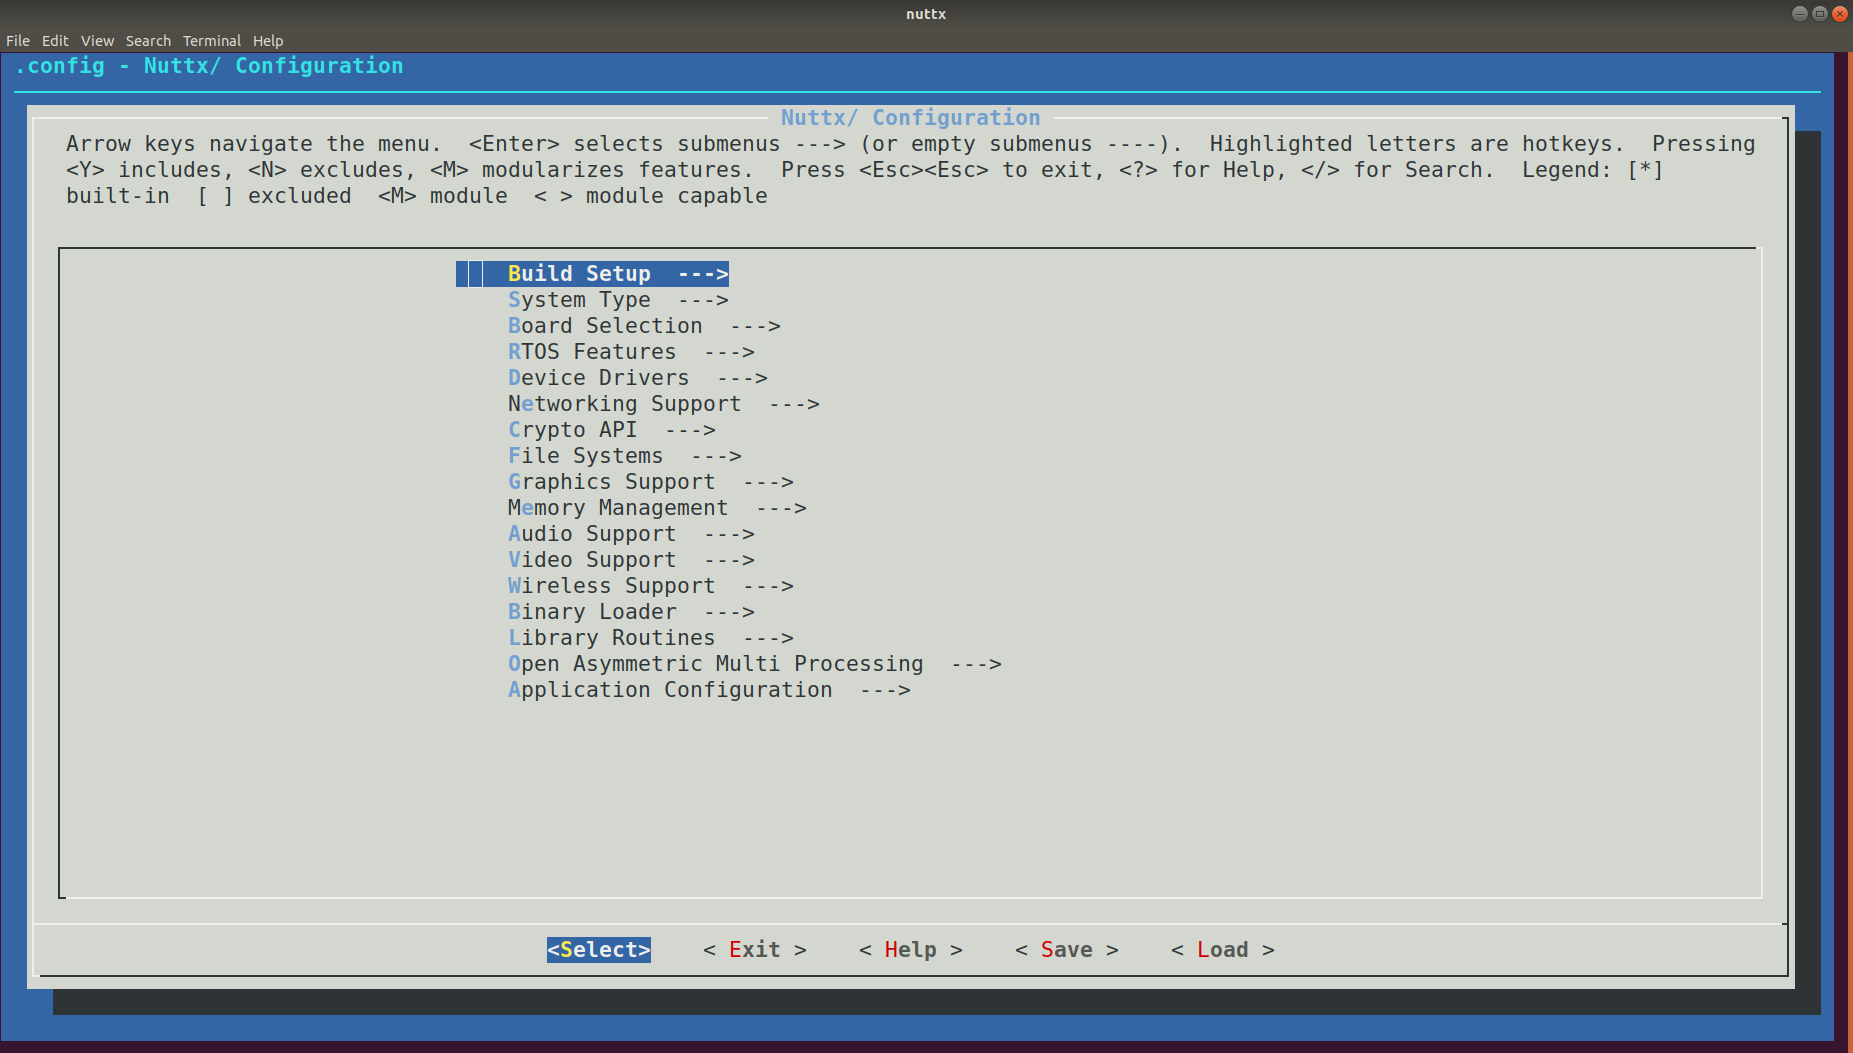
\includegraphics[width=0.75\linewidth]{make menuconfig.png}
    \caption{Enter Caption}
    \label{fig:placeholder}
\end{figure}
\textbf{Testing console:}

\begin{lstlisting}[language=bash]
# Connect via serial (UART4 on EVK board)
picocom -b 115200 /dev/ttyUSB0

# Expected output after M7 boots:
NShell (NSH) NuttX-12.x.x
nsh> 

# Test commands:
nsh> help
nsh> free
nsh> ps
\end{lstlisting}

% TODO: Add screenshot of NSH console boot messages

\textbf{Success! ✅} Console working reliably.

\subsection{I2C3 Bus Configuration}

\textbf{Goal:} Enable I2C3 bus for sensor communication (ADXL345 accelerometer).

\textbf{I2C3 hardware details:}
\begin{itemize}
    \item Pins: GPIO\_SAI5\_RXD0 (SDA), GPIO\_SAI5\_RXD1 (SCL)
    \item Base Address: 0x30A40000
    \item Clock: 24 MHz (default)
\end{itemize}

\textbf{Enable I2C driver in NuttX:}

\begin{lstlisting}[language=bash]
cd ~/nuttx-work/nuttx
make menuconfig

# Navigate to:
System Type -> iMX8M Peripheral Selection
[*] I2C3

Device Drivers -> I2C Driver Support
[*] I2C Driver Support
[*] I2C character driver
\end{lstlisting}

\textbf{Enable I2C tools for testing:}

\begin{lstlisting}[language=bash]
# In menuconfig:
Application Configuration -> NSH Library
Disable Built-in Commands
    [ ] Disable i2c  # Make sure NOT checked

Application Configuration -> System Libraries and NSH Add-Ons
[*] I2C tool
\end{lstlisting}

\textbf{Rebuild and test:}

\begin{lstlisting}[language=bash]
make clean
make -j$(nproc)

# Load to M7
sudo cp nuttx.bin /lib/firmware/
echo stop | sudo tee /sys/class/remoteproc/remoteproc0/state
echo start | sudo tee /sys/class/remoteproc/remoteproc0/state

# Connect to console
picocom -b 115200 /dev/ttyUSB0
\end{lstlisting}

\subsection{I2C Bus Scanning}

\textbf{Scan I2C3 bus for devices:}

\begin{lstlisting}[language=bash]
nsh> i2c dev 3 0x00
     0  1  2  3  4  5  6  7  8  9  a  b  c  d  e  f
00:          -- -- -- -- -- -- -- -- -- -- -- -- -- 
10: -- -- -- -- -- -- -- -- -- -- -- -- -- -- -- -- 
20: 20 -- -- -- -- -- -- -- -- -- -- -- -- -- -- -- 
30: -- -- -- -- -- -- -- -- -- -- -- -- -- -- -- -- 
40: -- -- -- -- -- -- -- -- -- -- -- -- -- -- -- -- 
50: 50 -- -- 53 -- -- -- -- -- -- -- -- -- -- -- -- 
60: -- -- -- -- -- -- -- -- -- -- -- -- -- -- -- -- 
70: -- -- -- -- -- -- -- --
\end{lstlisting}

\textbf{Devices detected:}
\begin{itemize}
    \item \textbf{0x20:} Unknown (possibly GPIO expander)
    \item \textbf{0x50:} Unknown (possibly EEPROM)
    \item \textbf{0x53:} ADXL345 Accelerometer ✅
\end{itemize}

% TODO: Add photo of ADXL345 connected to I2C3

\subsection{ADXL345 Accelerometer Verification}

\textbf{Read Device ID (should be 0xE5):}

\begin{lstlisting}[language=bash]
nsh> i2c get -a 53 -r 0 3 1
READ Bus: 3 Addr: 53 Subaddr: 00 Value: e5
\end{lstlisting}

Device ID correct! ADXL345 responding.

\subsection{RPMsg Integration Attempt}

\begin{important}
\textbf{RPMsg with NuttX: DID NOT WORK}

RPMsg communication between Linux (A53) and NuttX (M7) was attempted but unsuccessful.

\textbf{What was tried:}
\begin{itemize}
    \item NuttX RPMsg library configuration
    \item Linux kernel RPMsg TTY driver
    \item Shared memory buffer setup
    \item Resource table configuration
\end{itemize}

\textbf{What failed:}
\begin{itemize}
    \item NuttX could not establish RPMsg channel with Linux
    \item \texttt{/dev/ttyRPMSG0} did not appear
    \item MU interrupts not properly handled in NuttX
    \item VirtIO ring buffer initialization issues
\end{itemize}

\end{important}

\begin{docref}
\textbf{Potential Solution for Next Intern:}

NuttX RPMsg pull request with Linux kernel patches:

\url{https://github.com/apache/nuttx/pull/12235}

This PR includes:
\begin{itemize}
    \item Updated NuttX RPMsg implementation
    \item Linux kernel driver patches needed for compatibility
    \item Example configurations
    \item Documentation on integration
\end{itemize}

\textbf{Important:} The Linux kernel patches from this PR were NOT applied during this internship. They may be required to get RPMsg working properly.

Next intern should:
\begin{enumerate}
    \item Apply Linux kernel patches from PR \#12235
    \item Update NuttX to version with RPMsg fixes
    \item Test basic RPMsg channel creation
    \item Validate bidirectional communication
    \item Implement high-bandwidth streaming
\end{enumerate}
\end{docref}

\section{PX4 Flight Controller Integration}

\subsection{PX4 Port Attempt}

\begin{important}
\textbf{PX4 Status: INCOMPLETE }
Since PX4 is not compatible with imx8mp M7 by default. I tried to rewrite all the necessary files needed by copying similar builds

PX4 Autopilot integration was attempted but not even close to being successful. 
\end{important}

\subsection{What Was Attempted}

\textbf{1. Initial PX4 setup:}

\begin{lstlisting}[language=bash]
cd ~
git clone https://github.com/PX4/PX4-Autopilot.git --recursive
cd PX4-Autopilot
\end{lstlisting}

\textbf{2. Board configuration created:}

\begin{lstlisting}[language=bash]
# Created new board based on fmu-v6xrt template
mkdir -p boards/nxp/imx8mp-evk
cp -r boards/px4/fmu-v6xrt/* boards/nxp/imx8mp-evk/

# Copied working NuttX config
cp ~/nuttx-work/nuttx/boards/arm/mx8mp/verdin-mx8mp/configs/nsh/defconfig \
   boards/nxp/imx8mp-evk/nuttx-config/nsh/defconfig
\end{lstlisting}

\textbf{3. PX4 platform code additions:}

Added mx8mp chip detection in \texttt{platforms/nuttx/cmake/px4\_impl\_os.cmake}:

\begin{lstlisting}[language=cmake]
elseif(CONFIG_ARCH_CHIP_MX8MP)
    set(CHIP_MANUFACTURER "nxp")
    set(CHIP "mx8mp")
\end{lstlisting}

Created platform code:

\begin{lstlisting}[language=bash]
cd platforms/nuttx/src/px4/nxp/
cp -r rt117x mx8mp  # Used RT117x as template
\end{lstlisting}

\textbf{4. Critical discovery: PX4's embedded NuttX lacks mx8mp support!}

\begin{lstlisting}[language=bash]
# Copied mx8mp architecture files to PX4's embedded NuttX
cp -r ~/nuttx-work/nuttx/arch/arm/src/mx8mp \
   platforms/nuttx/NuttX/nuttx/arch/arm/src/

cp -r ~/nuttx-work/nuttx/arch/arm/include/mx8mp \
   platforms/nuttx/NuttX/nuttx/arch/arm/include/

# Fixed chip symlink
cd platforms/nuttx/NuttX/nuttx/arch/arm/src/
rm chip
ln -s mx8mp chip
\end{lstlisting}

\textbf{5. Minimal board configuration:}

Created \texttt{board\_config.h}:

\begin{lstlisting}[language=c]
#pragma once

#include <nuttx/config.h>
#include <px4_platform_common/px4_config.h>
#include <nuttx/compiler.h>
#include <stdint.h>
#include <arch/board/board.h>

#define BOARD_NAME "IMX8MP_EVK"
#define BOARD_HAS_CONTROL_STATUS_LEDS 0

__BEGIN_DECLS
__EXPORT const char *board_get_hw_type_name(void);
__EXPORT int board_get_hw_version(void);
__EXPORT int board_get_hw_revision(void);
__END_DECLS
\end{lstlisting}

\textbf{6. Disabled unsupported drivers:}

In \texttt{boards/nxp/imx8mp-evk/default.px4board}:

\begin{lstlisting}[language=python]
# Disabled drivers requiring chip-specific implementations:
# CONFIG_DRIVERS_UAVCAN=y         # CAN bus
# CONFIG_DRIVERS_ADC_BOARD_ADC=y  # ADC
# CONFIG_DRIVERS_DSHOT=y          # Motor control
# CONFIG_DRIVERS_PX4IO=y          # I/O coprocessor
# CONFIG_DRIVERS_TONE_ALARM=y     # Audio
\end{lstlisting}

\textbf{7. Build attempt:}

\begin{lstlisting}[language=bash]
cd ~/PX4-Autopilot
make clean
make nxp_imx8mp-evk_default
\end{lstlisting}

\subsection{Why PX4 Integration Failed}

\textbf{Multiple complex issues encountered:}

\begin{enumerate}
    \item \textbf{Board path configuration:}
    \begin{itemize}
        \item PX4's NuttX uses custom board directory structure
        \item \texttt{CONFIG\_ARCH\_BOARD\_CUSTOM\_DIR} path resolution issues
        \item Build system couldn't locate board files consistently
    \end{itemize}
    
    \item \textbf{Embedded NuttX vs standalone:}
    \begin{itemize}
        \item PX4 has its own NuttX fork with different structure
        \item Many mx8mp-specific files missing or incompatible
        \item Version mismatches between standalone NuttX and PX4's embedded version
    \end{itemize}
    
    \item \textbf{Driver dependencies:}
    \begin{itemize}
        \item PX4 expects many chip-specific drivers not ported to mx8mp
        \item Build system tightly coupled to supported platforms
        \item Missing: ADC, DShot, CAN, I/O coprocessor drivers
    \end{itemize}
 
\end{enumerate}

\subsection{Files Modified During PX4 Attempt}

\begin{verbatim}
PX4-Autopilot/
├── boards/nxp/imx8mp-evk/
│   ├── default.px4board              # Board configuration
│   ├── src/
│   │   ├── board_config.h           # Board definitions
│   │   ├── init.c                   # Initialization
│   │   └── CMakeLists.txt           # Build config
│   └── nuttx-config/nsh/defconfig   # NuttX config
├── platforms/nuttx/cmake/
│   └── px4_impl_os.cmake            # Added mx8mp detection
├── platforms/nuttx/src/px4/nxp/
│   └── mx8mp/                       # Platform code (from rt117x)
└── platforms/nuttx/NuttX/nuttx/
    └── arch/arm/
        ├── src/mx8mp/               # Architecture code
        └── include/mx8mp/           # Headers
\end{verbatim}


\subsection{Key Resources}

\begin{docref}
\textbf{Essential Documentation:}

\textbf{NXP Official:}
\begin{itemize}
    \item i.MX8MP Reference Manual
    \item AN5317: Using Cortex-M with Linux
    \item MCUXpresso SDK: \url{https://mcuxpresso.nxp.com}
\end{itemize}

\textbf{NuttX Resources:}
\begin{itemize}
    \item NuttX Documentation: \url{https://nuttx.apache.org/docs/}
    \item i.MX8MP Support PR: \url{https://github.com/apache/nuttx/pull/10486}
    \item RPMsg with kernel patches: \url{https://github.com/apache/nuttx/pull/12235}
    \item Community forum discussion: \url{https://lists.apache.org/thread/yj7jj7rz0svrnz8zn1nv1gzygz5gorkp}
    \item NuttX Google Groups (search: "imx8mp", "verdin-mx8mp")
\end{itemize}

\textbf{PX4 Resources (if attempting integration):}
\begin{itemize}
    \item PX4 Developer Guide: \url{https://docs.px4.io/main/en/}
    \item PX4 NXP Platform Code: RT117x implementation as reference
    \item MAVLink Protocol: \url{https://mavlink.io/}
\end{itemize}

\textbf{Working nuttx elf:}
\begin{itemize}
    \item GitHub (bare-metal): \url{https://github.com/yulyuri/firmware-and-dts/blob/master/nuttx-m7-uart4-i2c.elf}
    \item NuttX configuration (in home directory backup)
\end{itemize}


\end{docref}




\chapter{Conclusion and Support}

\section{Wrapping Up}

You've reached the end of this documentation! Yay!




\section{Documentation}

\begin{gitref}
\textbf{LaTeX Source Code Available:}

The complete LaTeX source for this documentation will be included in the GitHub repository:

\url{https://github.com/yulyuri/firmware-and-dts}

Why this matters:
\begin{itemize}
    \item You can update it as you make progress
    \item Fix any possible errors I made or unclear sections
    \item Add your own discoveries and of course help future interns/ anyone working on this
\end{itemize}
\end{gitref}

\section{Getting Help}

\subsection{Contact me}

If you get stuck or have some questions:

My contact information is at the beginning of this document. Just send an email, I'm happy to help clarify things. I was struggling very hard

\subsection{NXP Community Forums - Your Best Friend}

\begin{important}
\textbf{The NXP Community Forums Are very helpful:}

\url{https://community.nxp.com/}

The NXP forums saved me countless times during this internship. I asked \textbf{god knows how many questions} there, and the community is incredibly helpful.

\end{important}


\section{Final Words}

This has been an incredibly rewarding internship. The i.MX8M Plus is a powerful platform, and you now have the foundation to build amazing things with it. IGood luck with the project. I hope you are able to learn and have as much fun as I did.

\vspace{0.5cm}

\begin{flushright}
\textit{Chyn}\\
\textit{December 2025}\\
\end{flushright}

% TODO: Add photo of final working setup
% TODO: Add photo of team/workspace
\vspace{2cm}
\end{document}